\documentclass[]{article}
\usepackage[utf8]{inputenc}
\usepackage[ngerman]{babel}
\usepackage[T1]{fontenc}
\usepackage{%
	ngerman,
	ae,
	times,  %% hier kann man die Schriftart einstellen
	graphicx,
	url,
	scrlayer-scrpage,
	lastpage,
	mathtools,
	geometry,
	multicol,
	cancel,
	xcolor,
	nicematrix,
	xfrac,
	tikz,
	pgfplots,
	amsmath,
	colortbl,
	centernot,
	dsfont,
	textgreek,
	icomma,
	pdfpages,
	kvmap}
\usepackage[hidelinks]{hyperref}
\usepackage[thinlines]{easybmat}
\usetikzlibrary{datavisualization}
\usetikzlibrary{datavisualization.formats.functions}
\usetikzlibrary{intersections}
\pgfplotsset{compat=1.17}
\newcommand{\del}[1]{\cancel{~#1~}}
\NiceMatrixOptions{ last-col,code-for-last-col = \color{blue}\scriptstyle,light-syntax}
\newlength\dlf
\newcommand\alignedhighlight[3]{
  % #1 = color
  % #2 = before alignment
  % #3 = after alignment
  &
  \begingroup
  \settowidth\dlf{$\displaystyle #2$}
  \addtolength\dlf{\fboxsep+\fboxrule}
  \hspace{-\dlf}
  \fcolorbox{#1}{#1}{$\displaystyle #2 #3$}
  \endgroup
}
\newcommand{\reference}[1]{ \text{\small{\textcolor{blue}{(#1)}}} }

\newcommand{\topic}{Mathematik 1}
\newcommand{\subtopic}{Zusammenfassung}
\newcommand{\authors}{-}

%Head and Footnotes
\setlength{\headheight}{2.1\baselineskip} %baselineskip = minimum distance bbetween the bottom of one line to another.
\geometry{bottom = 3cm}
\setlength{\headsep}{\baselineskip}
\ihead[\topic\hrule]{\topic\hrule}
\chead[\subtopic\\~]{\subtopic\\~}
\ohead[\authors\\~]{\authors\\~}
\ifoot[\hyperlink{toc}{Zurück zum Inhaltsverzeichnis}]{\hyperlink{toc}{Zurück zum Inhaltsverzeichnis}}
\cfoot[~]{~}
\ofoot[Seite \thepage~von \pageref{LastPage}]{Seite \thepage~von \pageref{LastPage}}

%Paragraph spacings
\setlength{\parindent}{0em} %em = with of an 'M'
\setlength{\parskip}{1ex} %ex = height of an 'x'


\newcommand{\V}{\lor}
\newcommand{\A}{\land}
\newcommand{\T}[1]{\overline{#1}}
\newcommand{\eq}{\Leftrightarrow}
\newcommand{\rarr}{\Rightarrow}
\newcommand{\red}[1]{\textcolor{red}{#1}}

\newcommand{\unit}[1]{\text{#1}}
\newcommand{\fracunit}[2]{\frac{\unit{#1}}{\unit{#2}}}
\newcommand{\textsq}[1]{\ensuremath{\text{#1}^2}}
\newcommand{\textpow}[2]{\ensuremath{\text{#1}^{#2}}}
\newcommand{\tdot}{\ensuremath{\cdot}}


\begin{document}
\tableofcontents
\addtocontents{toc}{\protect\hypertarget{toc}{}}
\pagebreak
\section{Vorlesung 1 (06.10.2020)}
\subsection{Definition: Menge, Mengenelemente, leere Menge}
\subsection{Venn-Diagramme}
\subsection{Definition: Aussage}
\subsection{Definition: Aussageverknüpfung}
\subsection{Beispiele: Verneinung, Konjunktion, Desjunktion, Implikation, Äquivalenz}
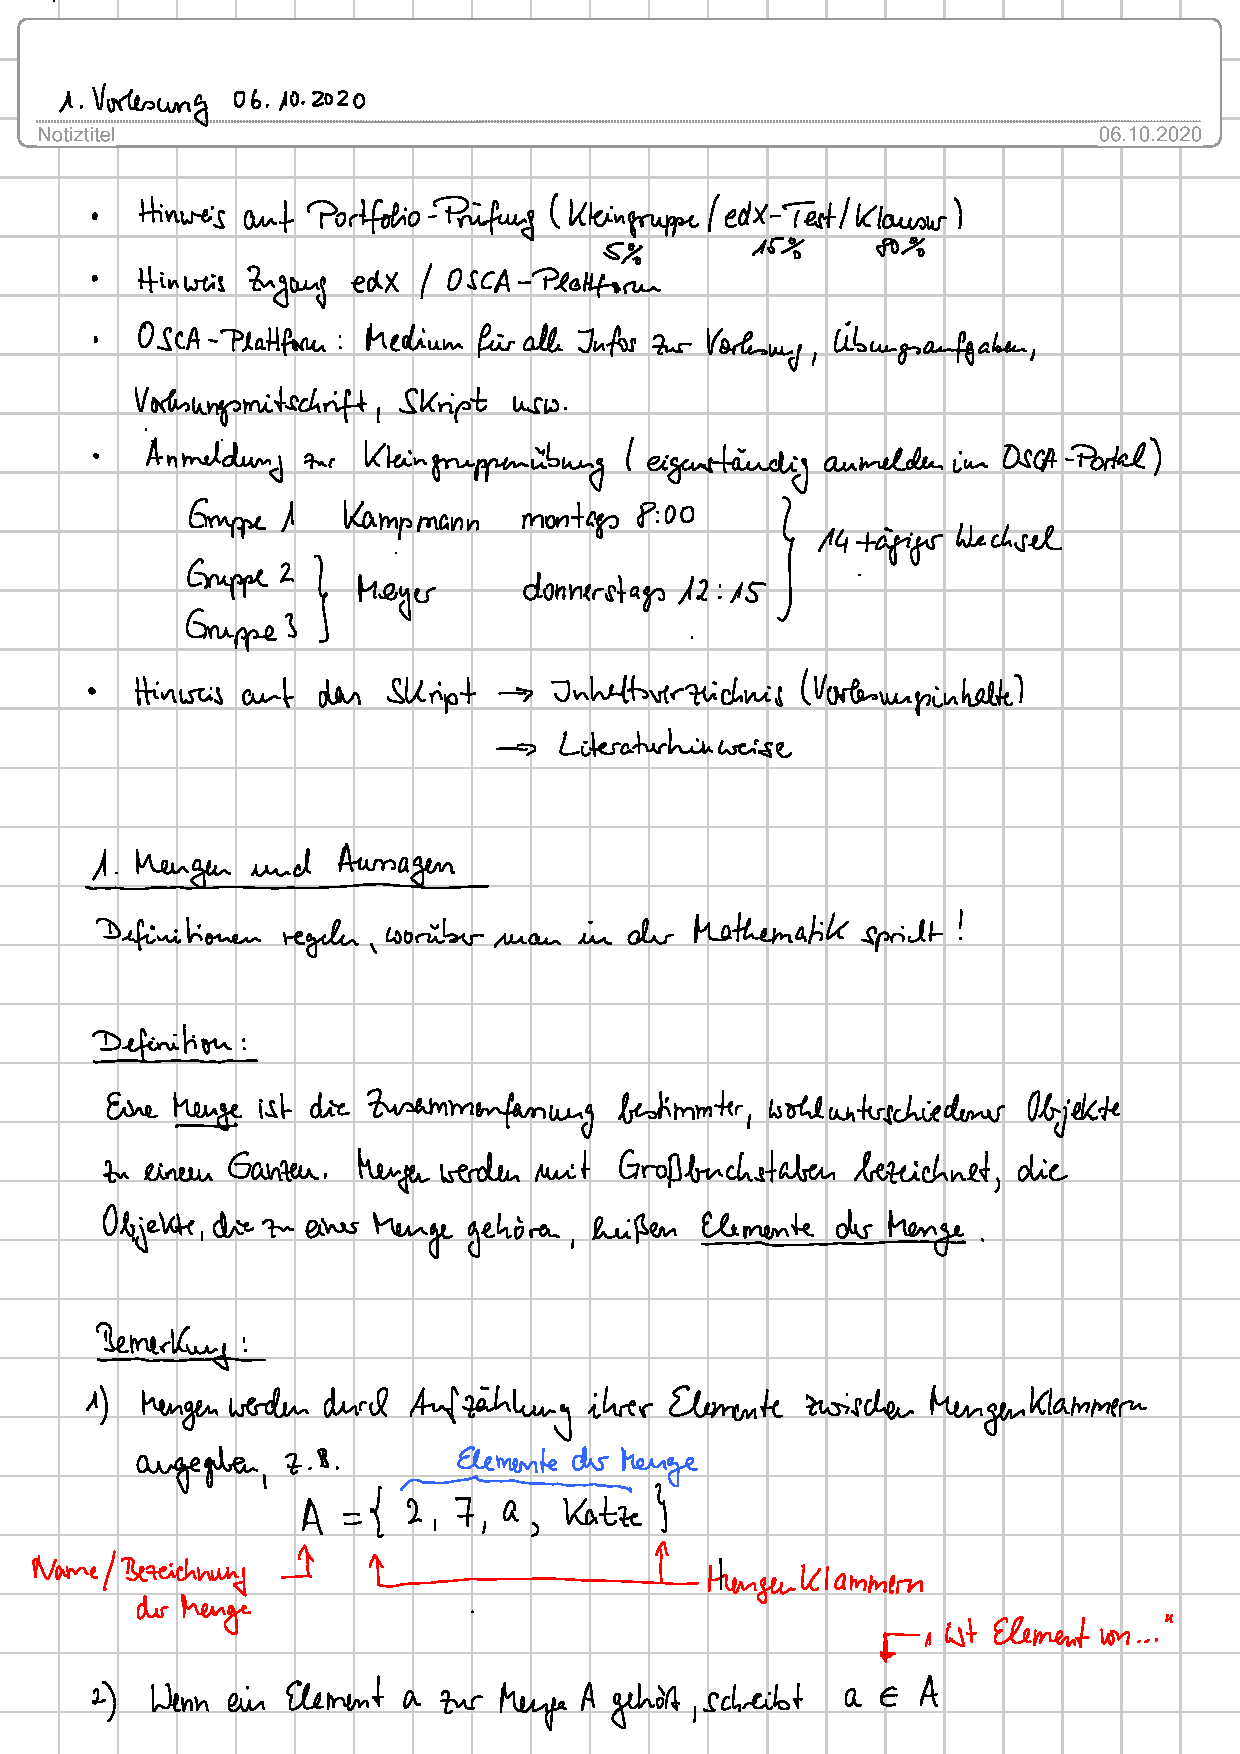
\includepdf[pages=-]{Mitschriften/1. Vorlesung 06.10.2020}

\section{Vorlesung 2 (07.10.2020)}
\subsection{Aussagenlogik: Tautologie, XOR, Allquantor, Existenzquantor}
\subsection{Rechenregeln für Aussageverknüpfung}
\subsection{Axiomatische Mengenlehre (Zermelo-Fraenkel)}
\subsection{Definition: Potenzmenge}
\subsection{Definition: Rechnen mit Mengen - Vereinigung, Durchschnitt, Differenz, Komplement}
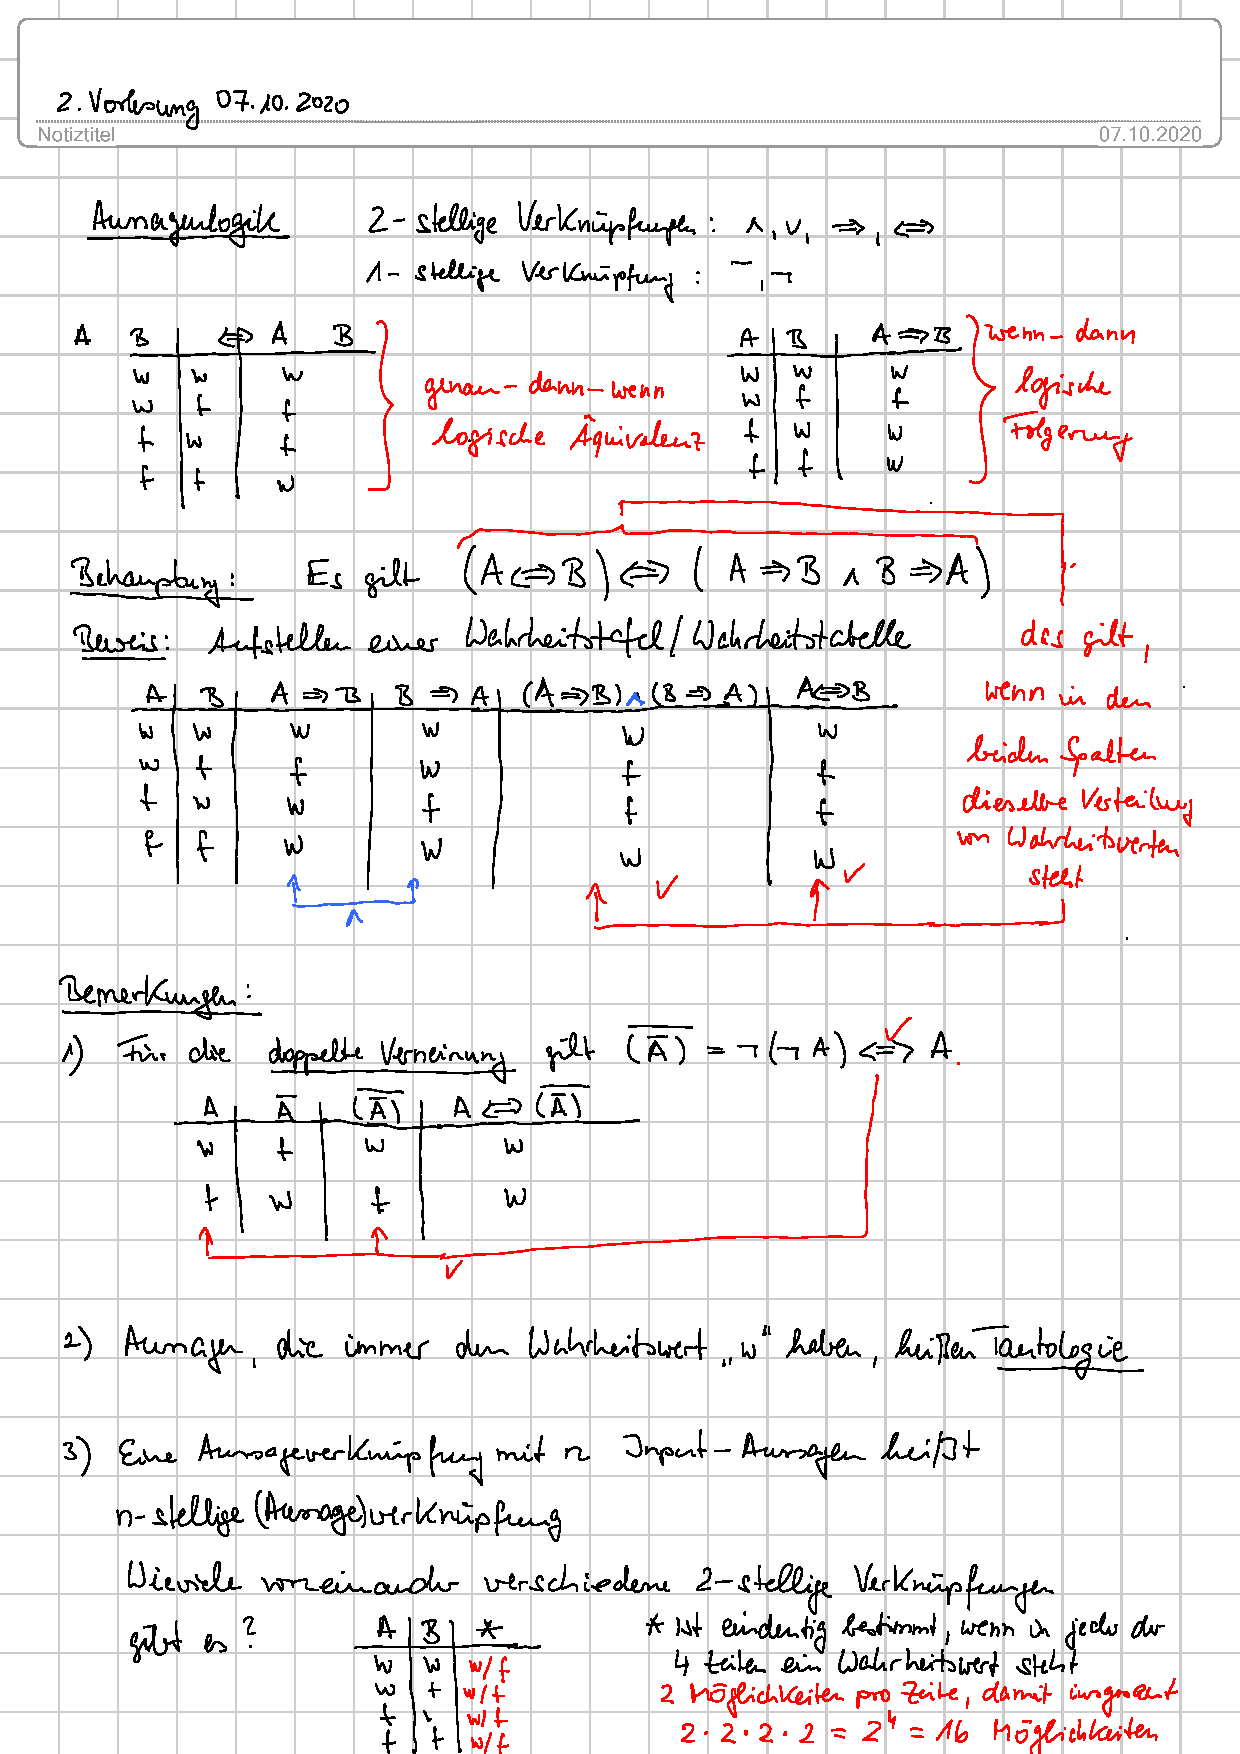
\includepdf[pages=-]{Mitschriften/2. Vorlesung 07.10.2020}

\section{Vorlesung 3 (12.10.2020)}
\subsection{Zahlenmengen}
\subsection{Definition: Aussageform}
\subsection{Definition: Kartesisches Produkt von Mengen, Tupel}
\subsection{Zahlenstrahl, Anordnung von Zahlen}
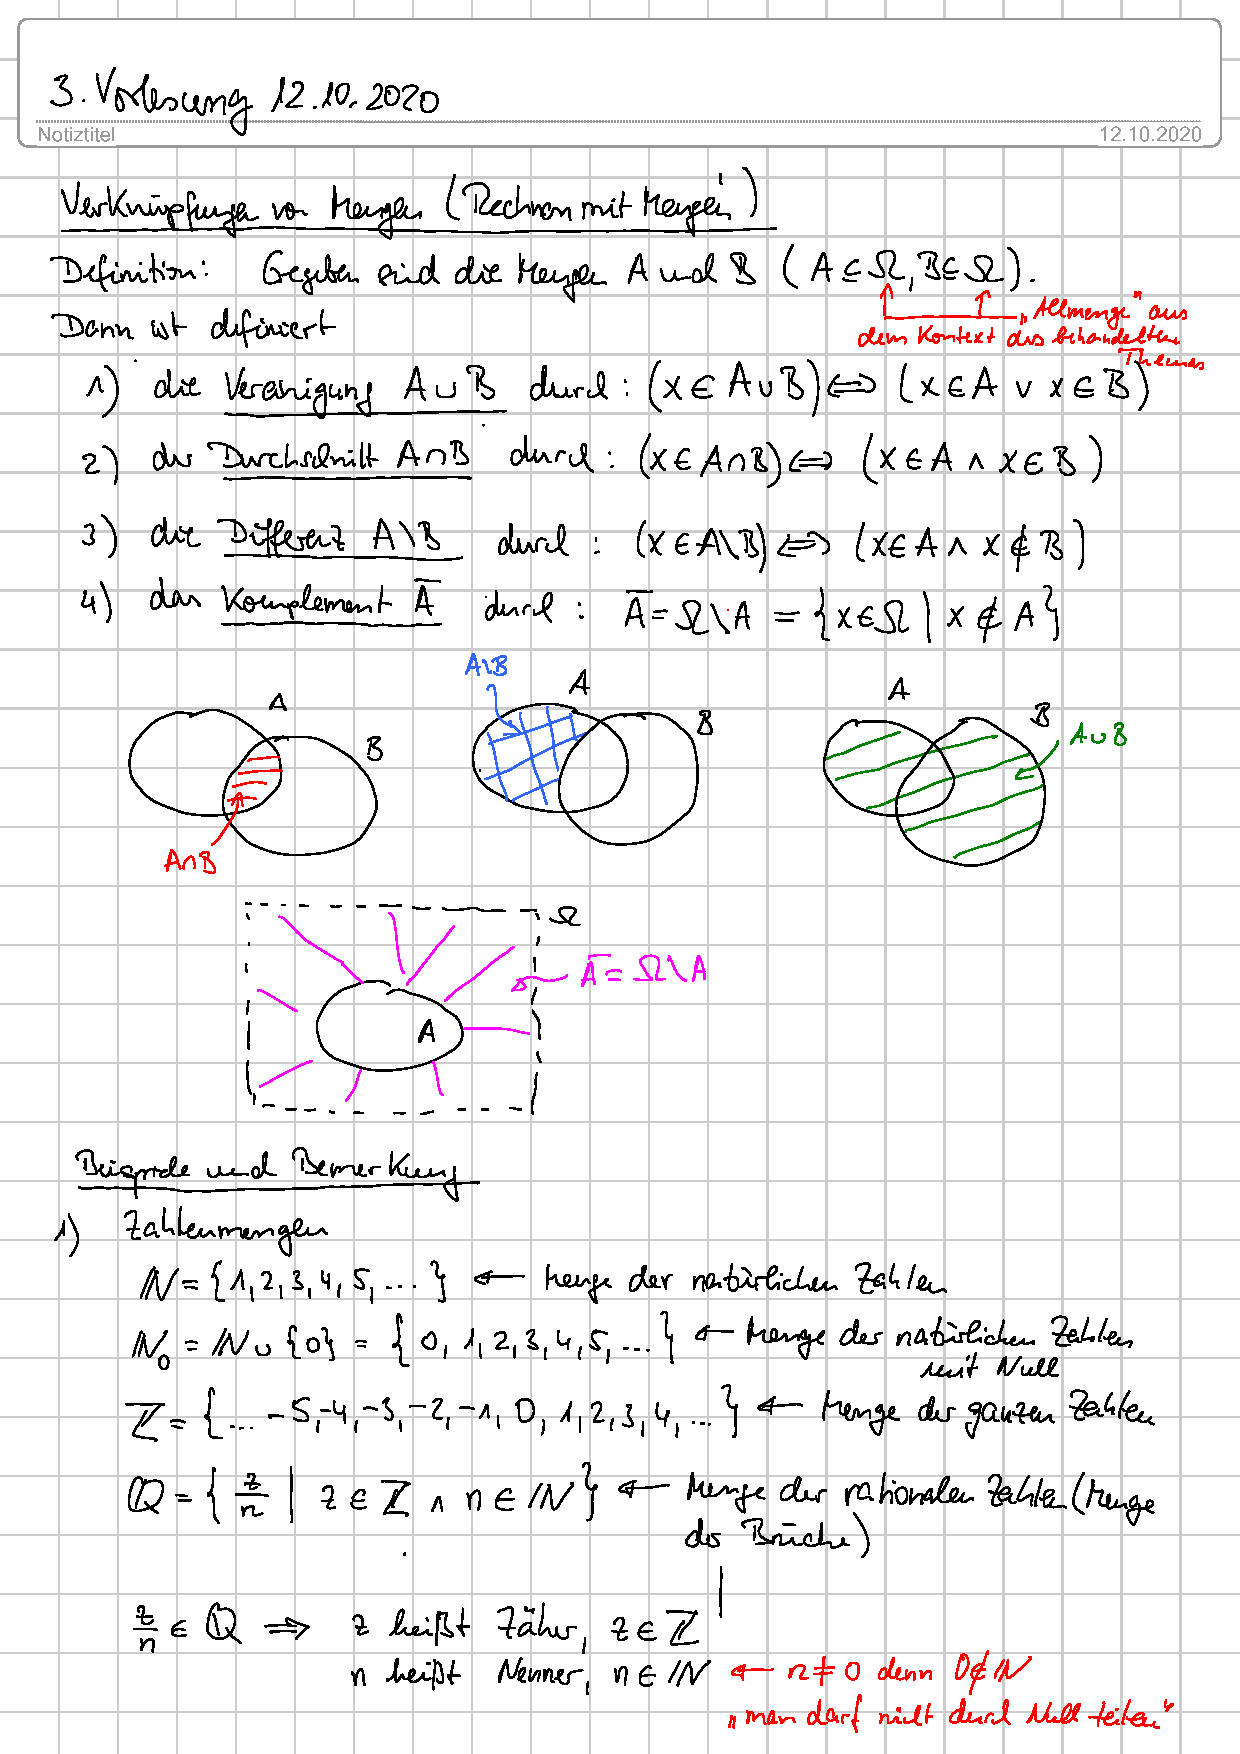
\includepdf[pages=-]{Mitschriften/3. Vorlesung 12.10.2020}

\section{Vorlesung 4 (13.10.2020)}
\subsection{Beipiele Relationen + Kartesisches Produkt}
\subsection{Definition: reflexiv, transitiv, symmetrisch, antisymmetrisch: Äquivalenzrelation, Ordnungsrelation}
\subsection{Definition: Äquivalenzklasse}
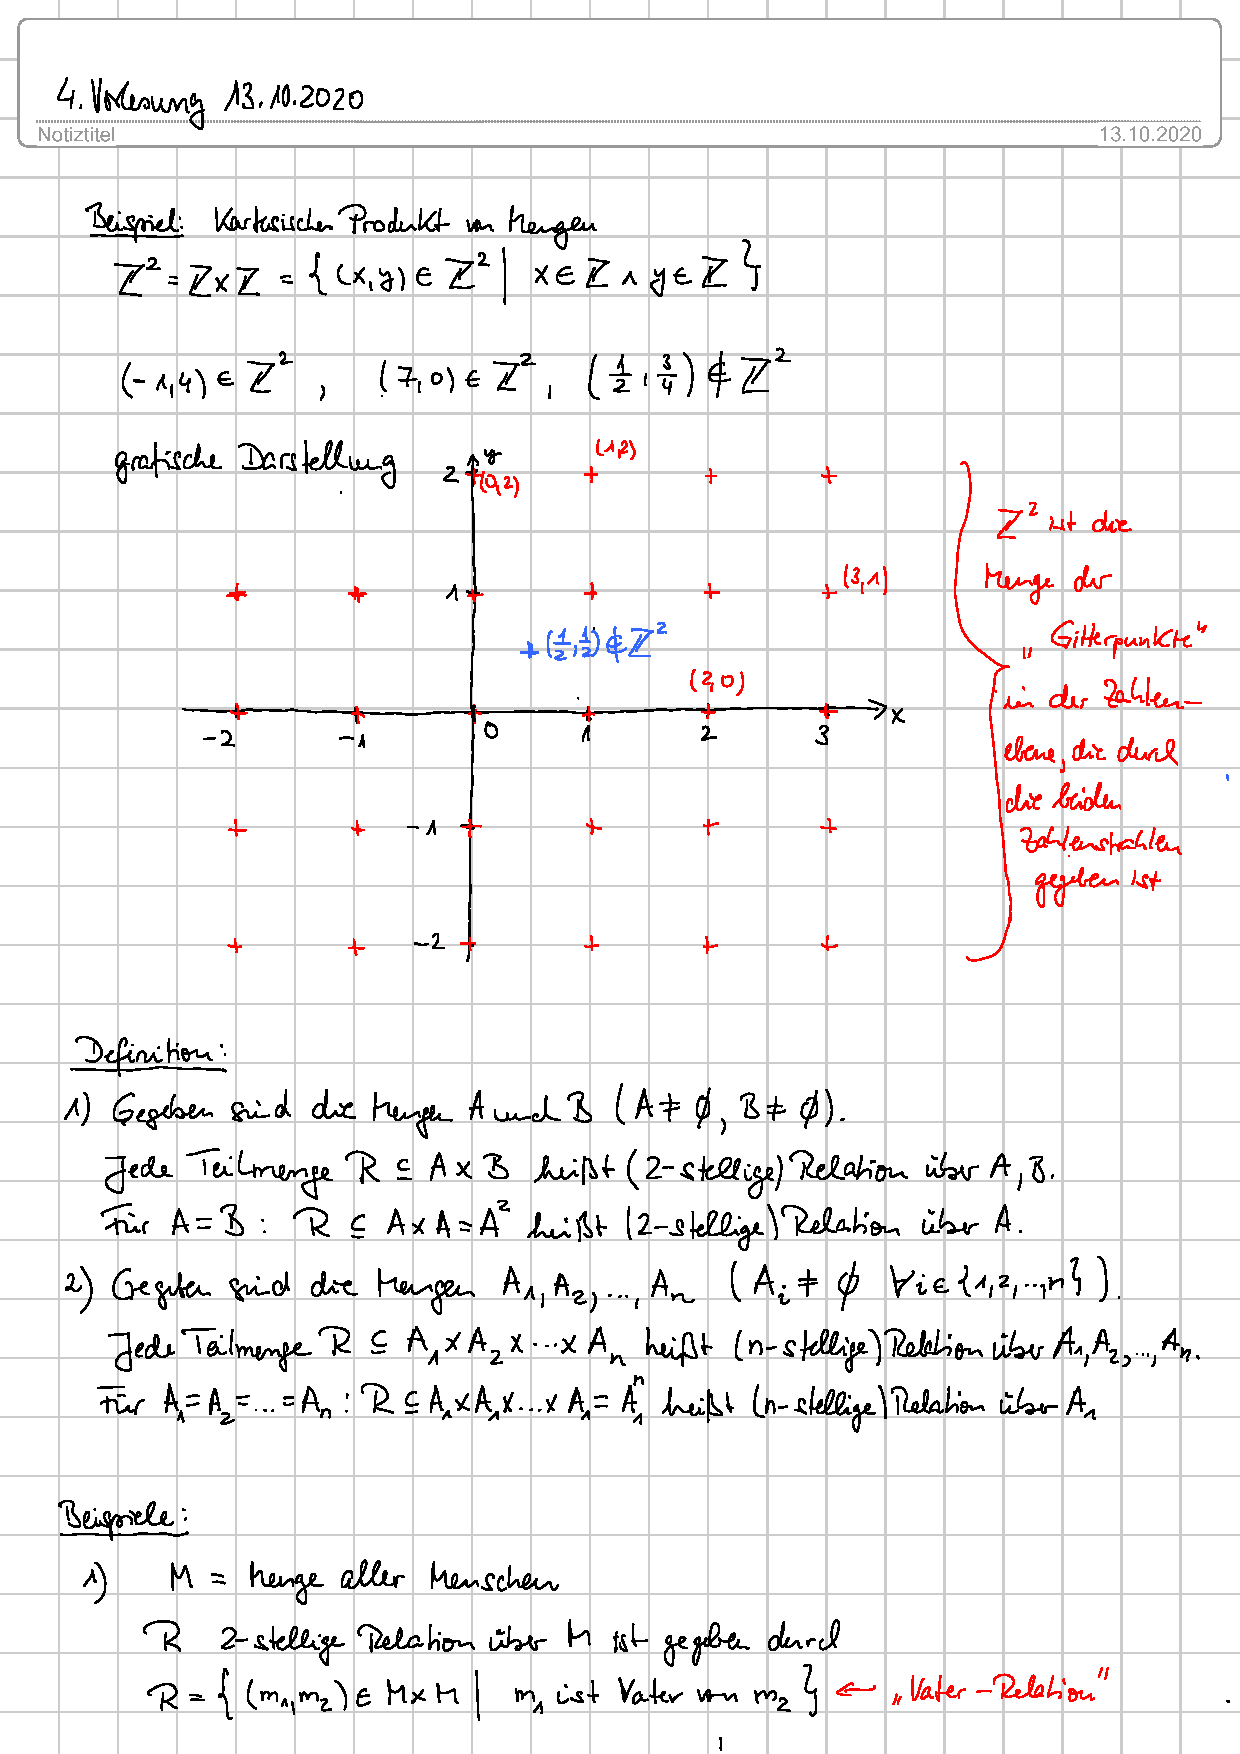
\includepdf[pages=-]{Mitschriften/4. Vorlesung 13.10.2020}

\section{Vorlesung 5 (14.10.2020)}
\subsection{Beipiele Äquivalenzklasse}
\subsection{Definition: vollständige Mengenpartition}
\subsection{Satz: Aquivalenzklassen bilden vollständige Mengenpartition}
\subsection{Definition: Verknüpfung}
\subsection{Definition: Abbildung, Funktion, Bild, Graph, Urbild}
\subsection{grafische Veranschaulichtung der reellen Zahlen}
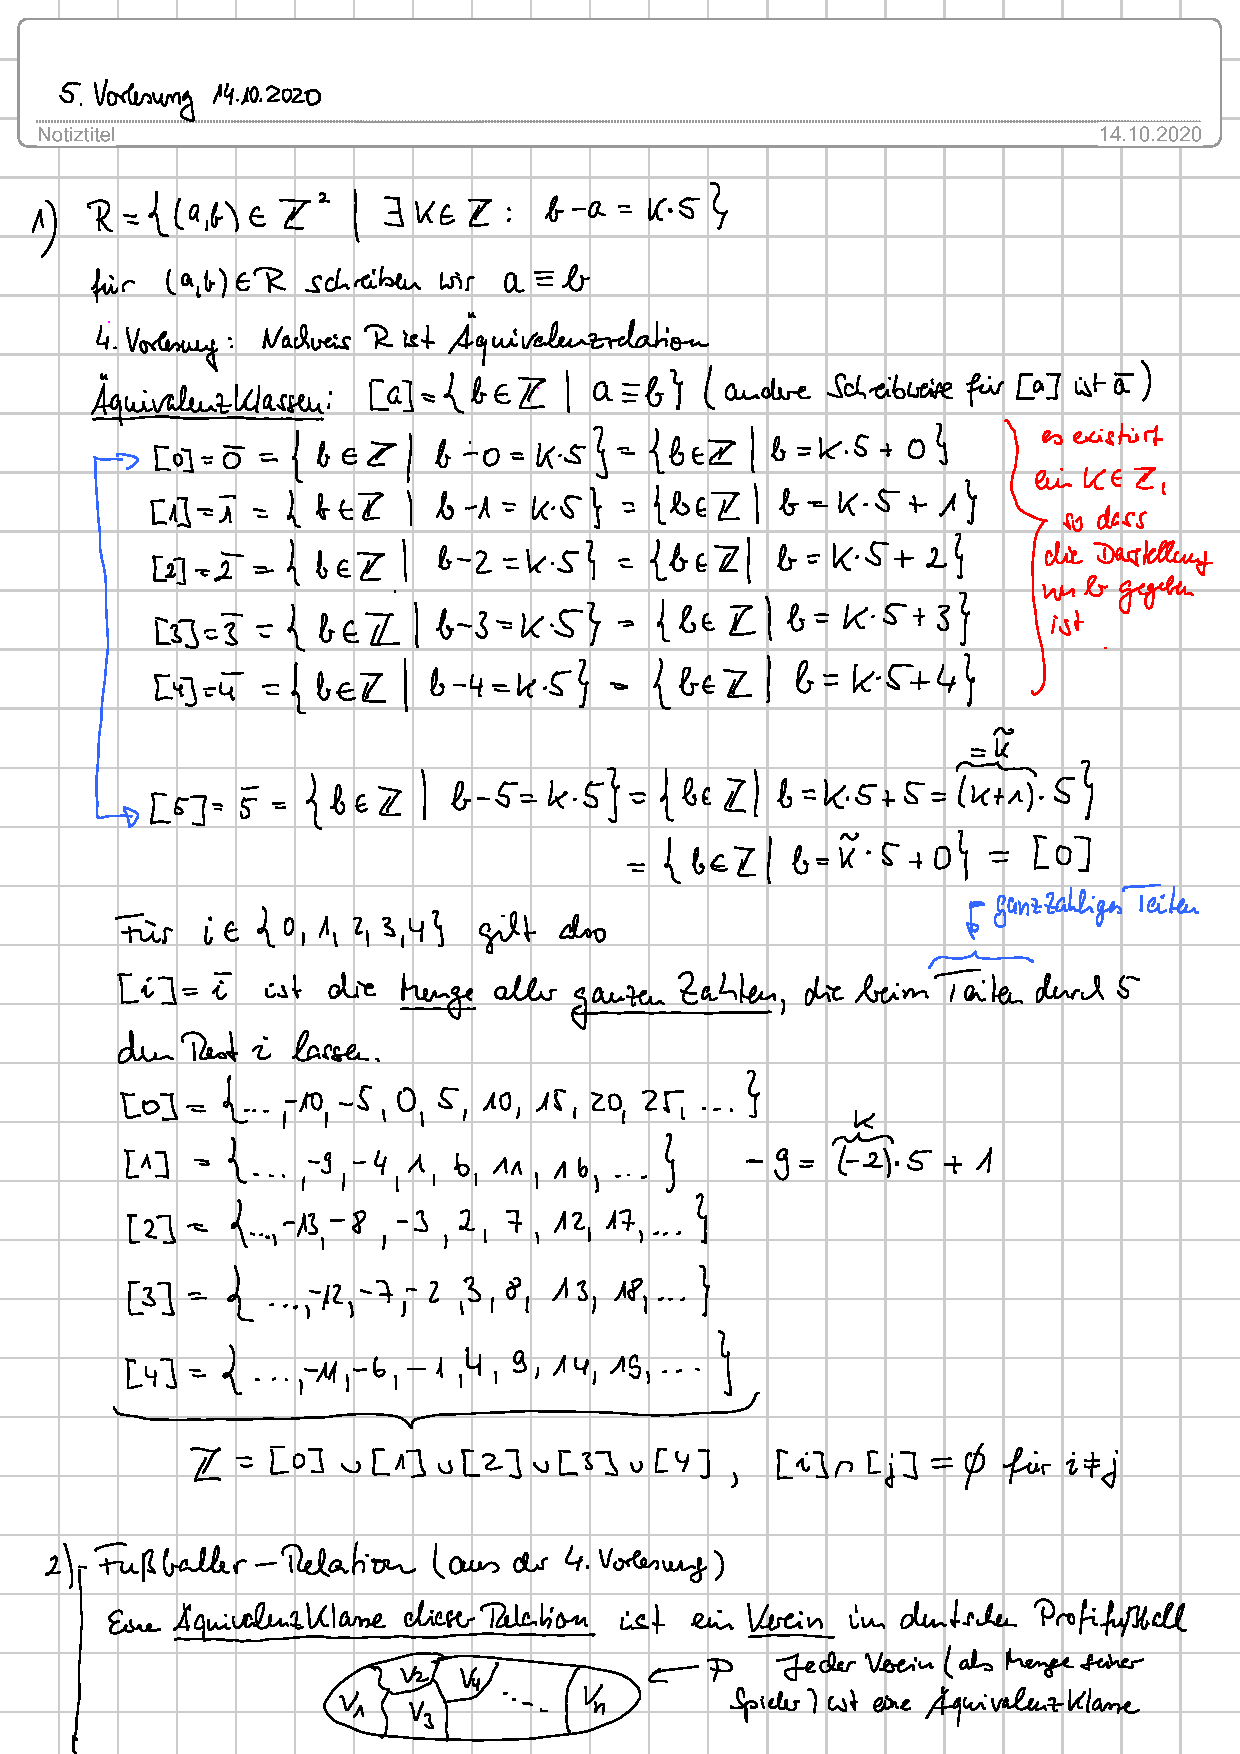
\includepdf[pages=-]{Mitschriften/5. Vorlesung 14.10.2020}

\section{Vorlesung 6 (19.10.2020)}
\subsection{Beipiele Abbildung, Funktion}
\subsection{Zahlensysteme}
\subsection{Peano-Axiome (natürliche Zahlen definieren)}
\subsection{Rechenregeln in den natürlichlen Zahlen}
\subsection{Definition: Endliche Summe}
\subsection{5. Peano-Axiom / Induktionsaxiom / vollständige Induktion}
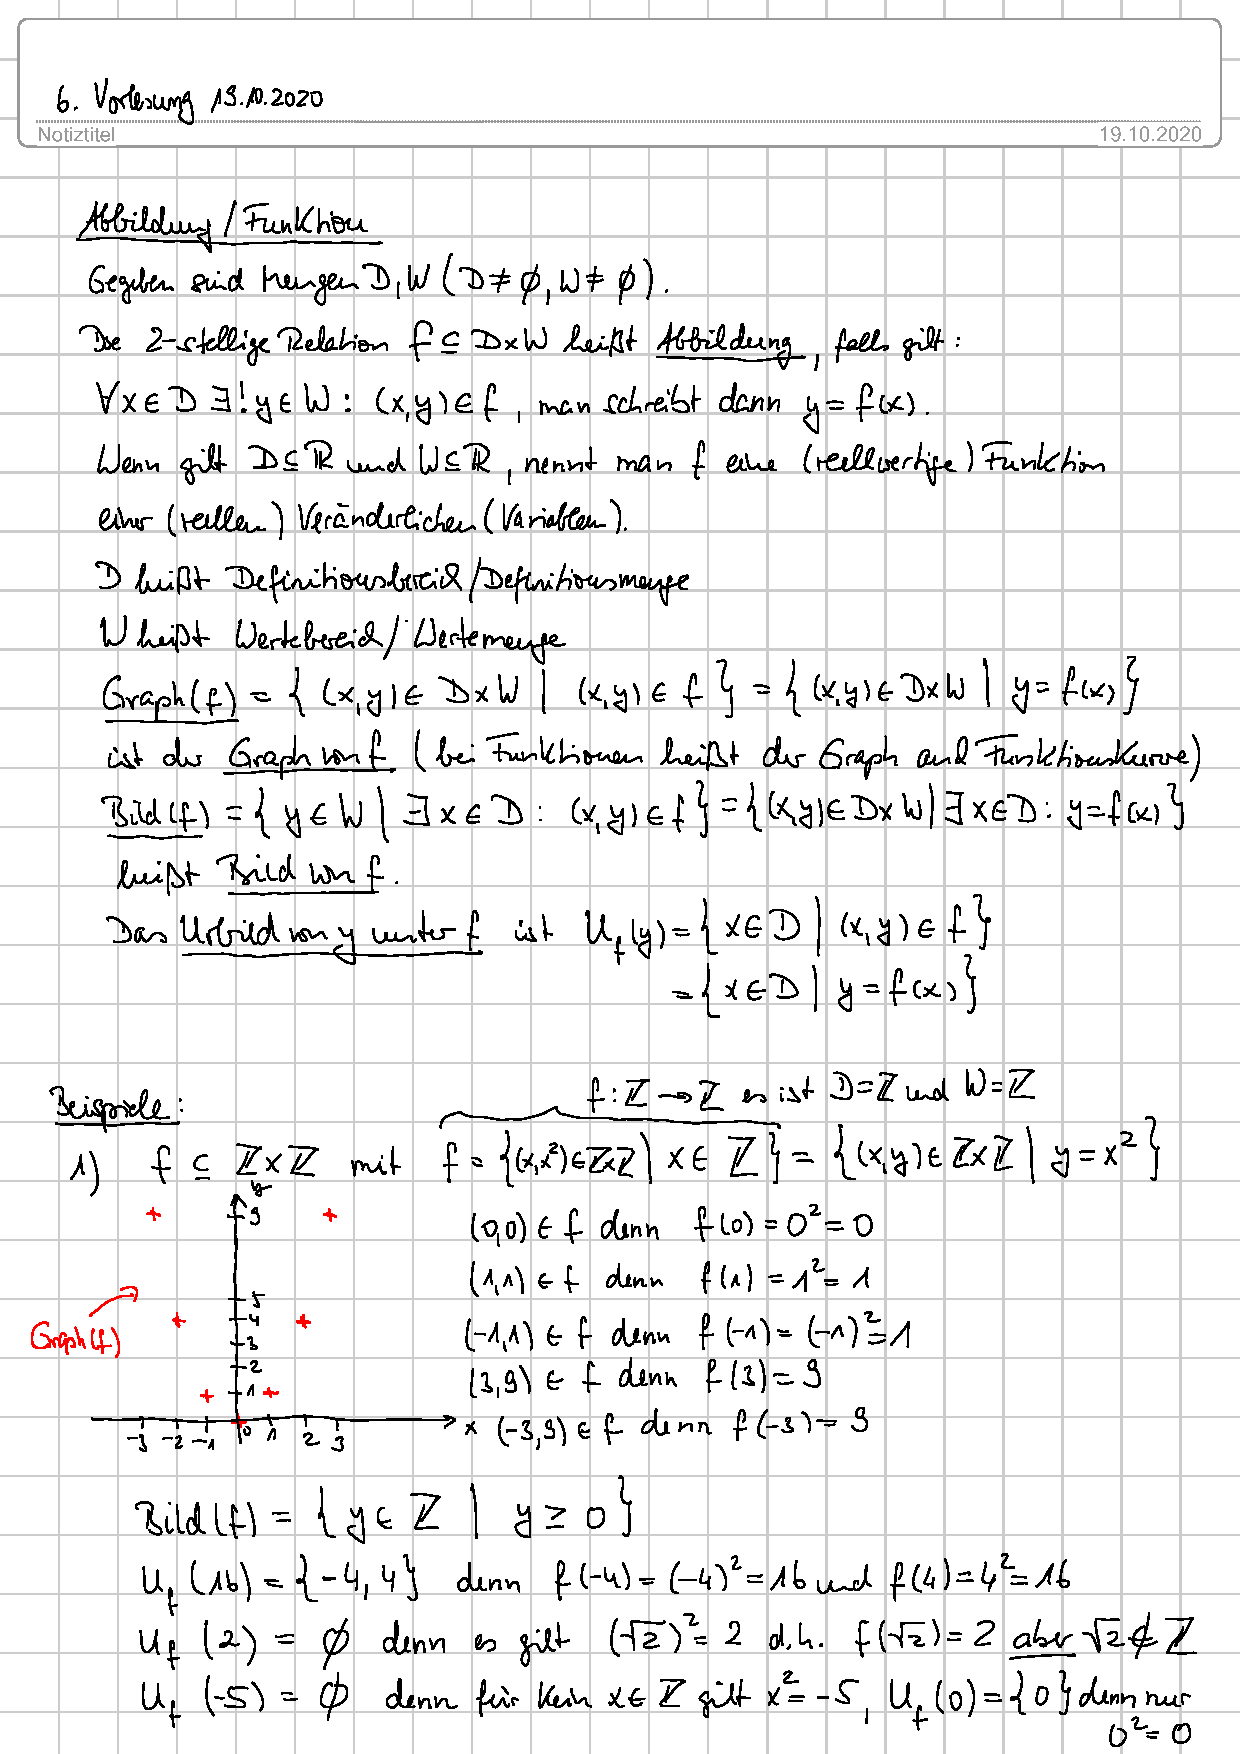
\includepdf[pages=-]{Mitschriften/6. Vorlesung 19.10.2020}

\section{Vorlesung 7 (20.10.2020)}
\subsection{Beipiele Vollständige Induktion}
\subsection{Definition durch Rekursion + Beispiele}
\subsection{Binomialkoeffizient}
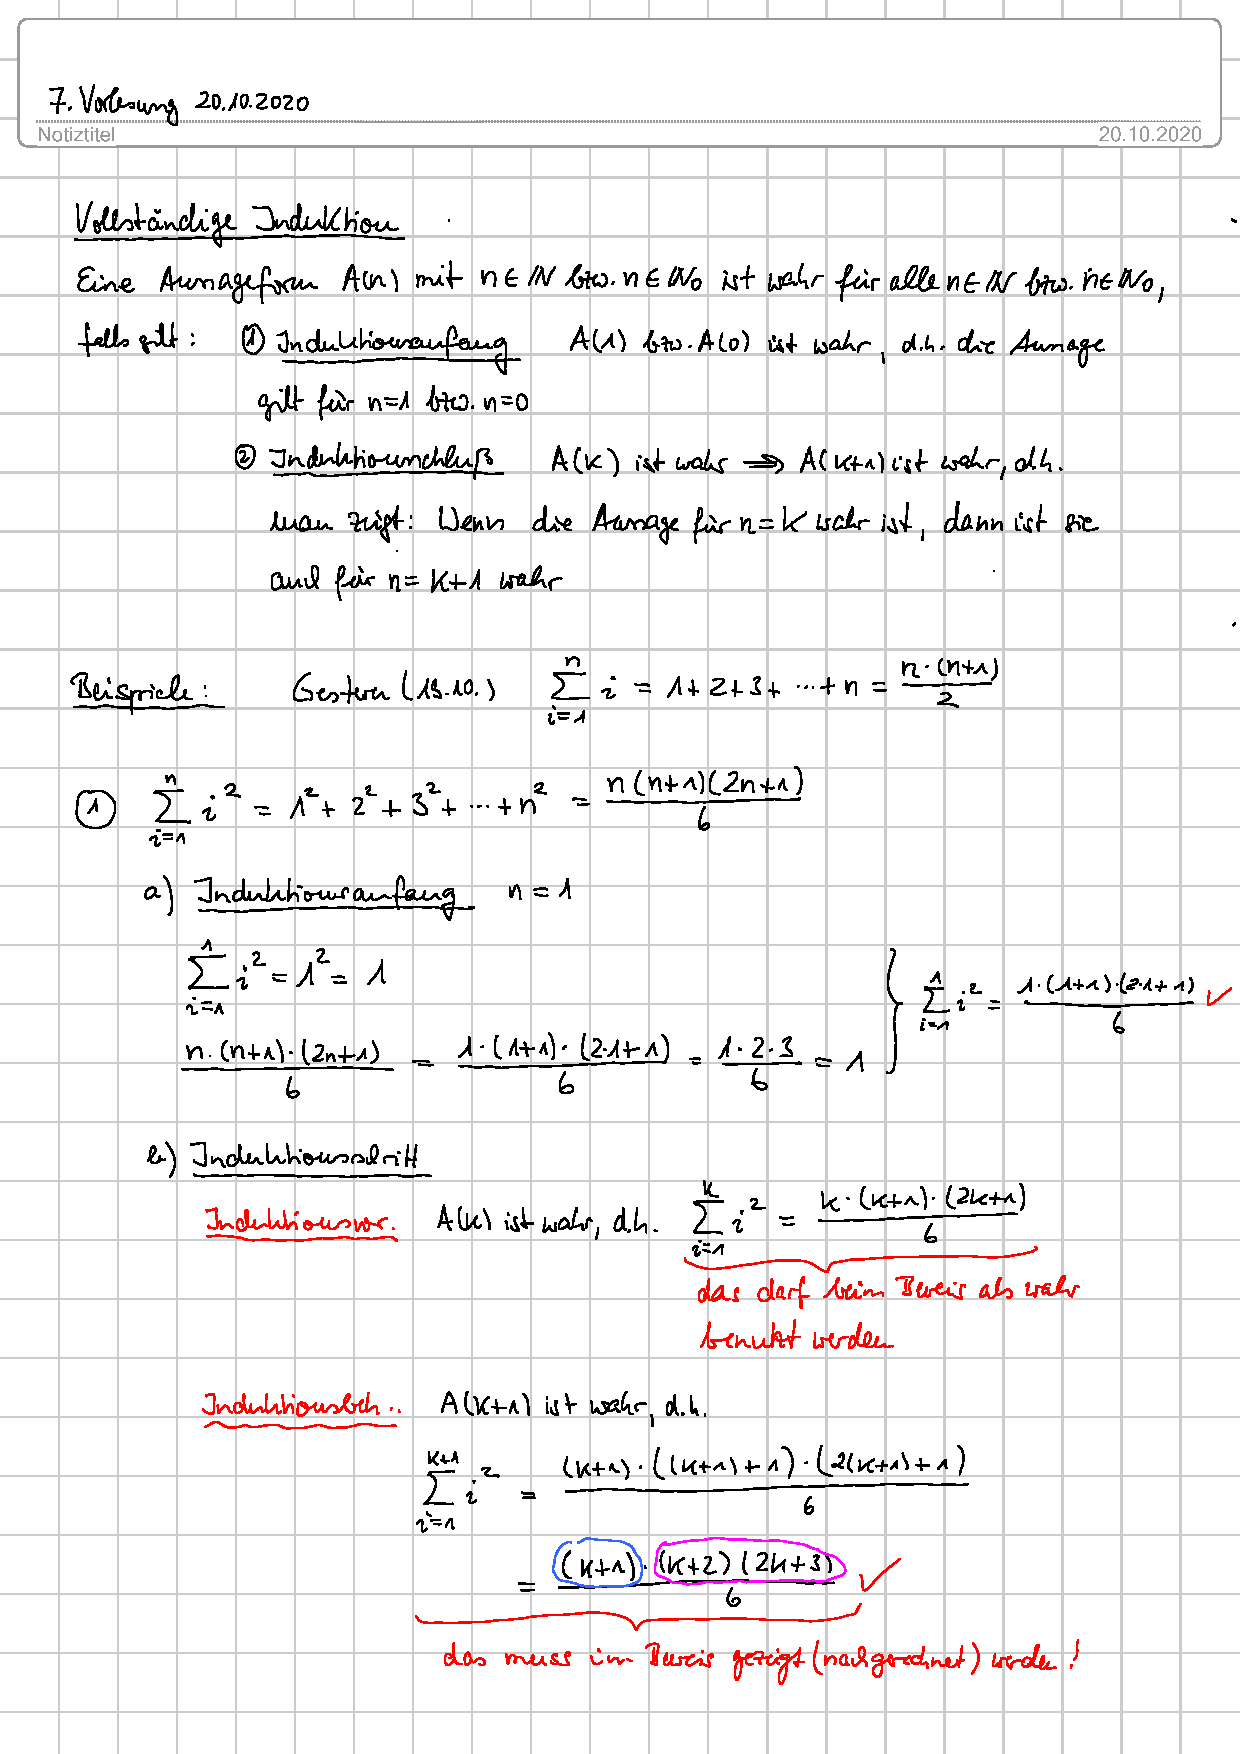
\includepdf[pages=-]{Mitschriften/7. Vorlesung 20.10.2020}

\section{Vorlesung 8 (21.10.2020)}
\subsection{Binomialkoeffizienten und Fakultät}
\subsection{Eigenschaften Binomialkoeffizient}
\subsection{Pascalsches Dreieck}
\subsection{1. Binomische Formel (+ 1. allgemeine Binomische Formel)}
\subsection{2. Binomische Formel (+ 2. allgemeine Binomische Formel)}
\subsection{Wiederholung: Ordnungsrelation, Vollständige Induktion}
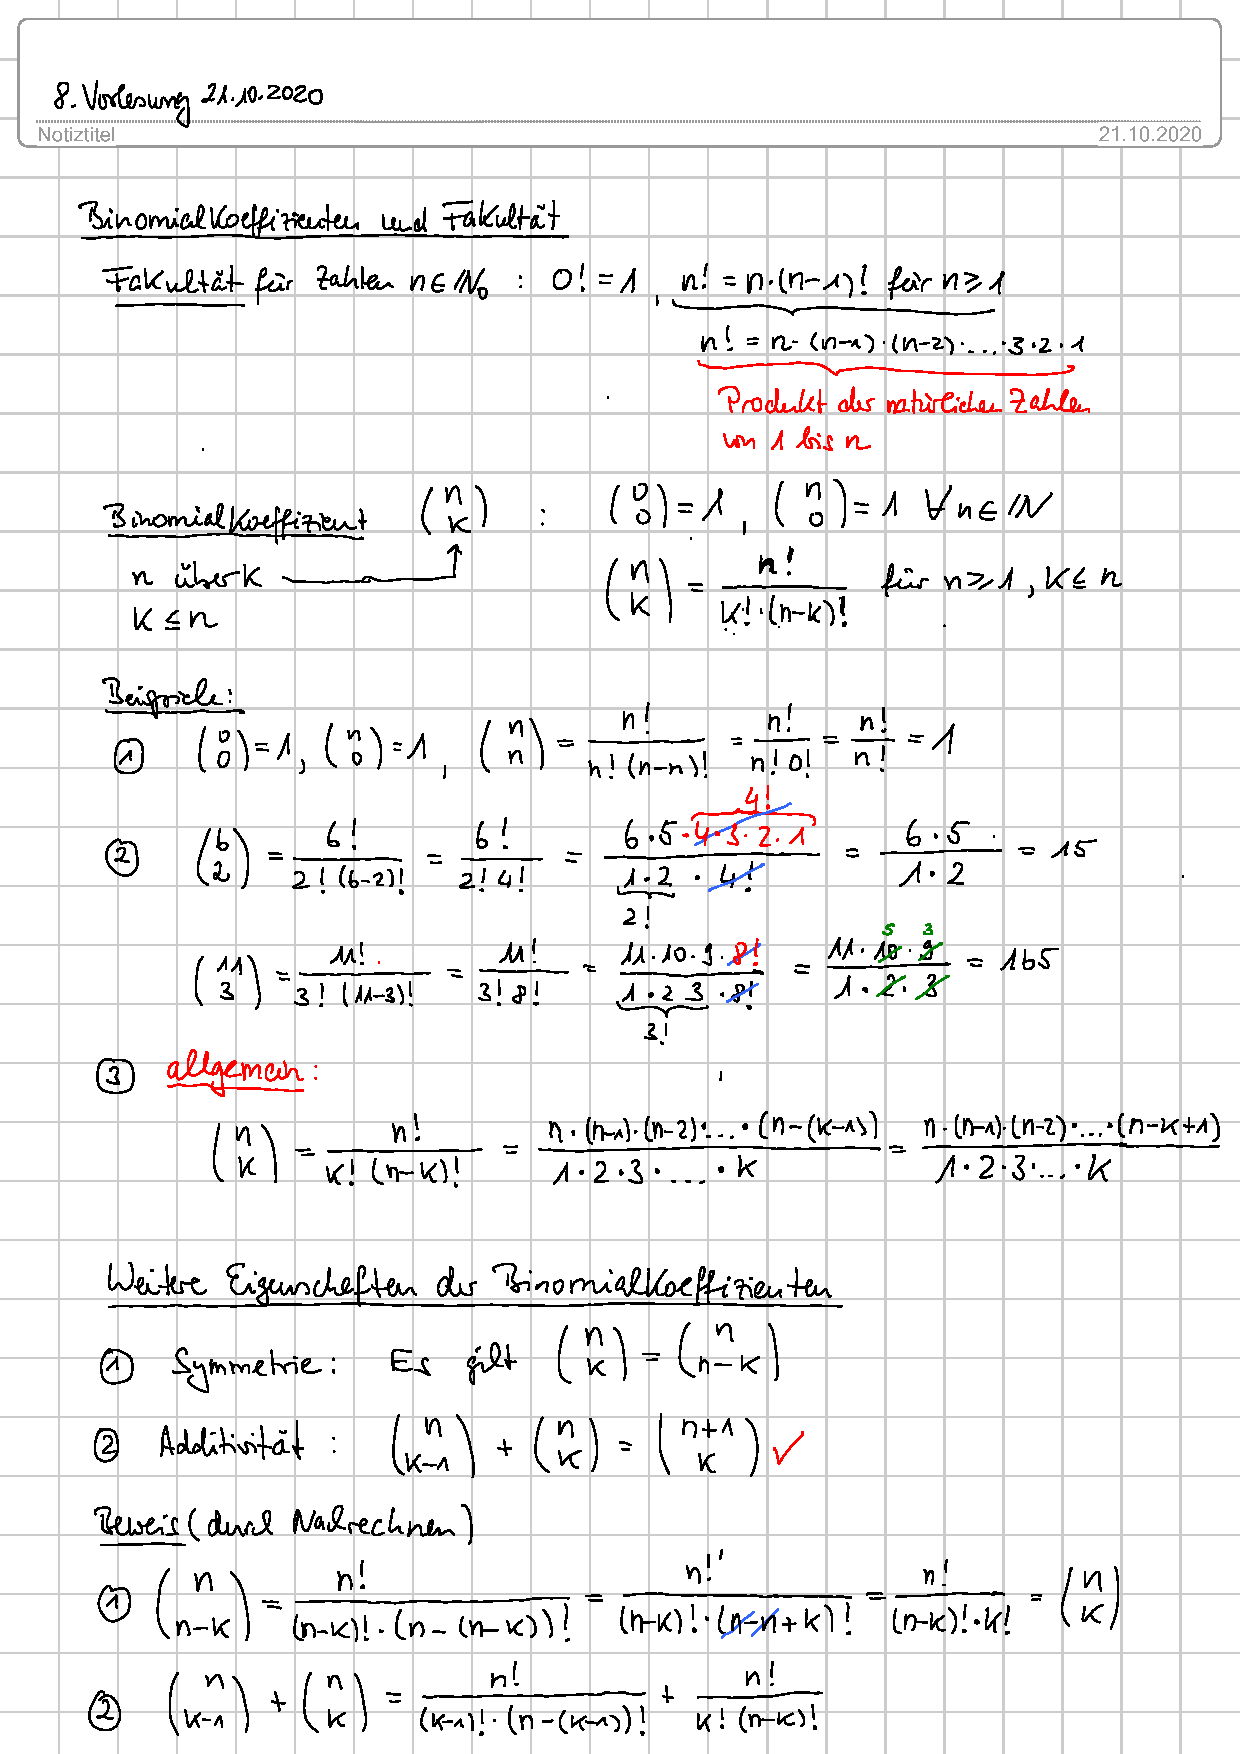
\includepdf[pages=-]{Mitschriften/8. Vorlesung 21.10.2020}

\section{Vorlesung 9 (26.10.2020)}
\subsection{Rechenregeln für Potenzen}
\subsection{3. Binomische Formel (+ 3. allgemeine Binomische Formel)}
\subsection{Elementares Multiplikationsprinzip}
\subsection{Elementare Kombinatorik (Anordnung, Auswahl)}
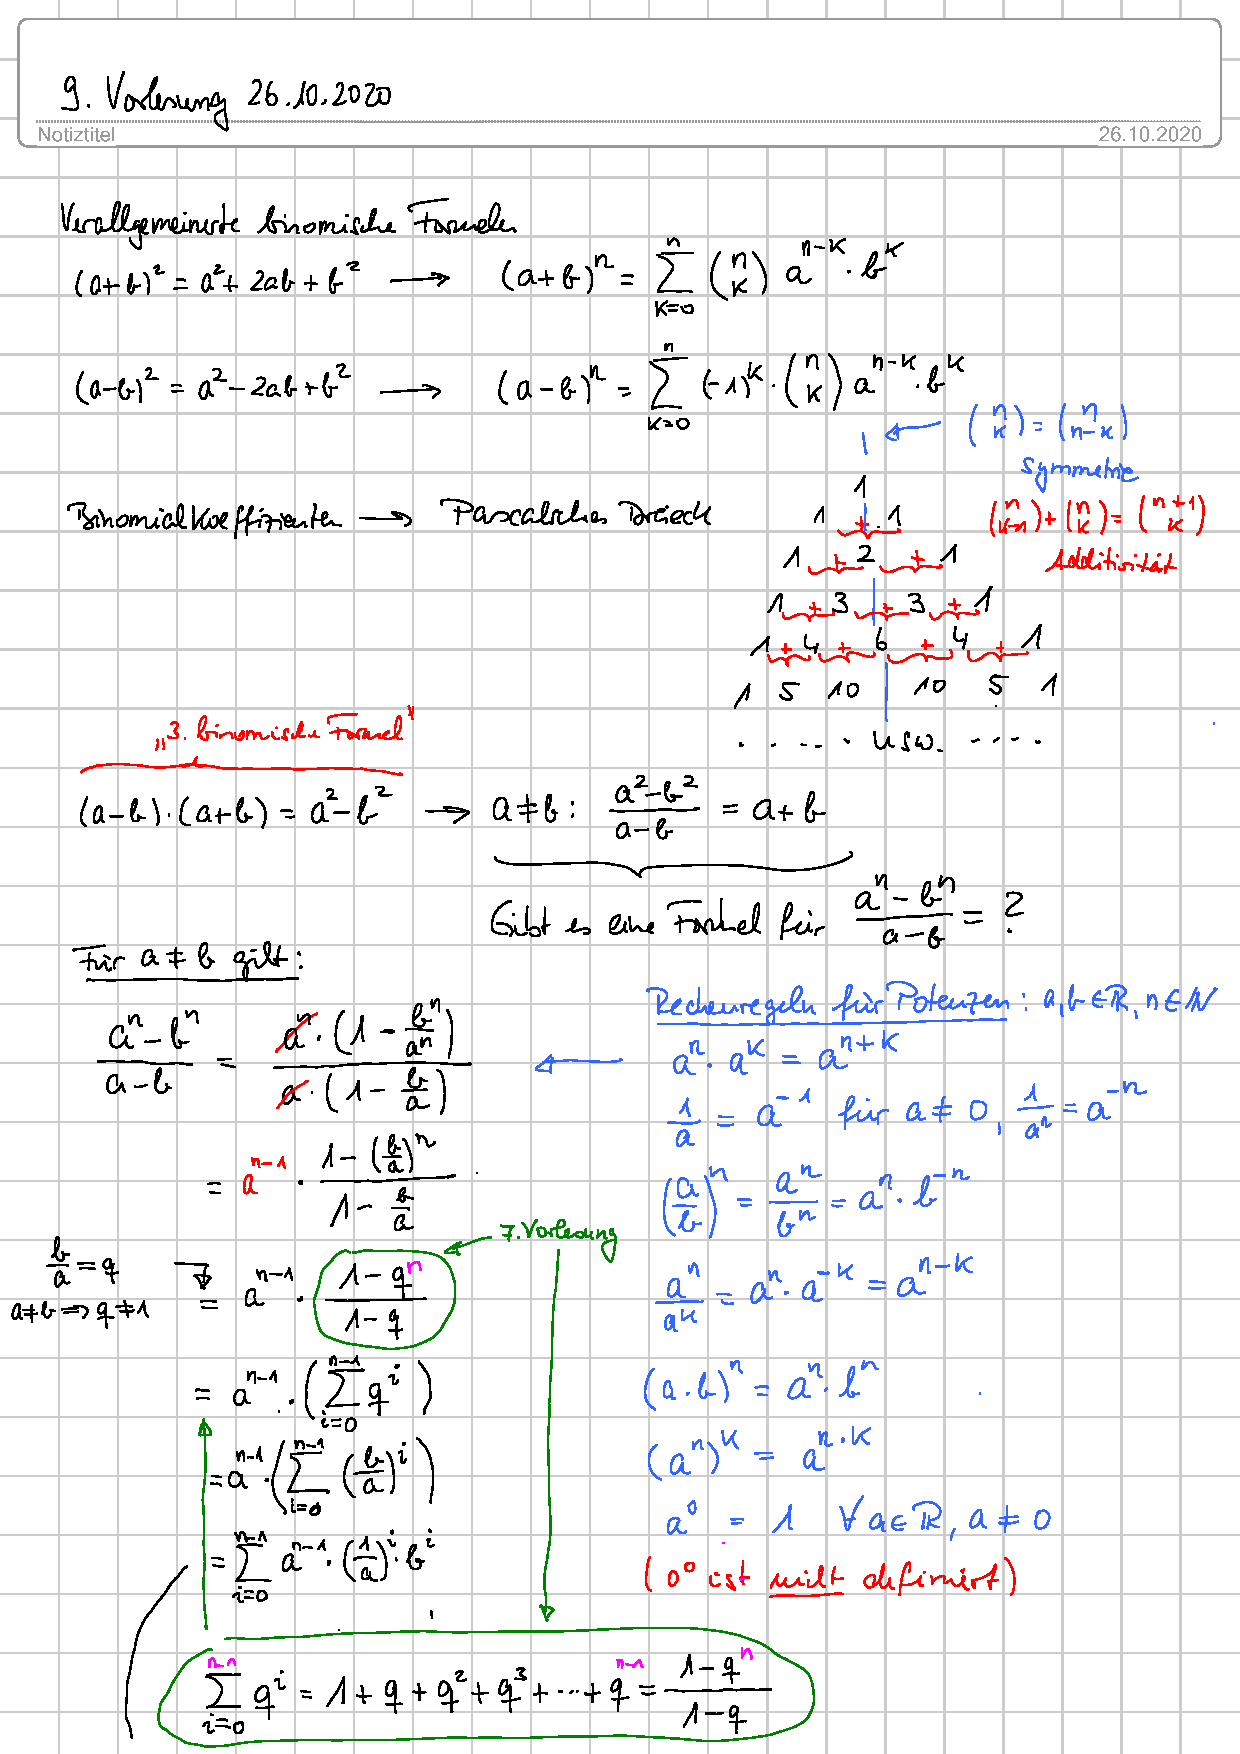
\includepdf[pages=-]{Mitschriften/9. Vorlesung 26.10.2020}

\section{Vorlesung 10 (27.10.2020)}
\subsection{Zusammenfassung Elementare Kombinatorik}
\subsection{Dezimaldarstellung rationaler Zahlen}
\subsection{Rechenregeln in den reellen Zahlen}
\subsection{Bemerkung: Was ist ein Körper, Anordnungsaxiom}
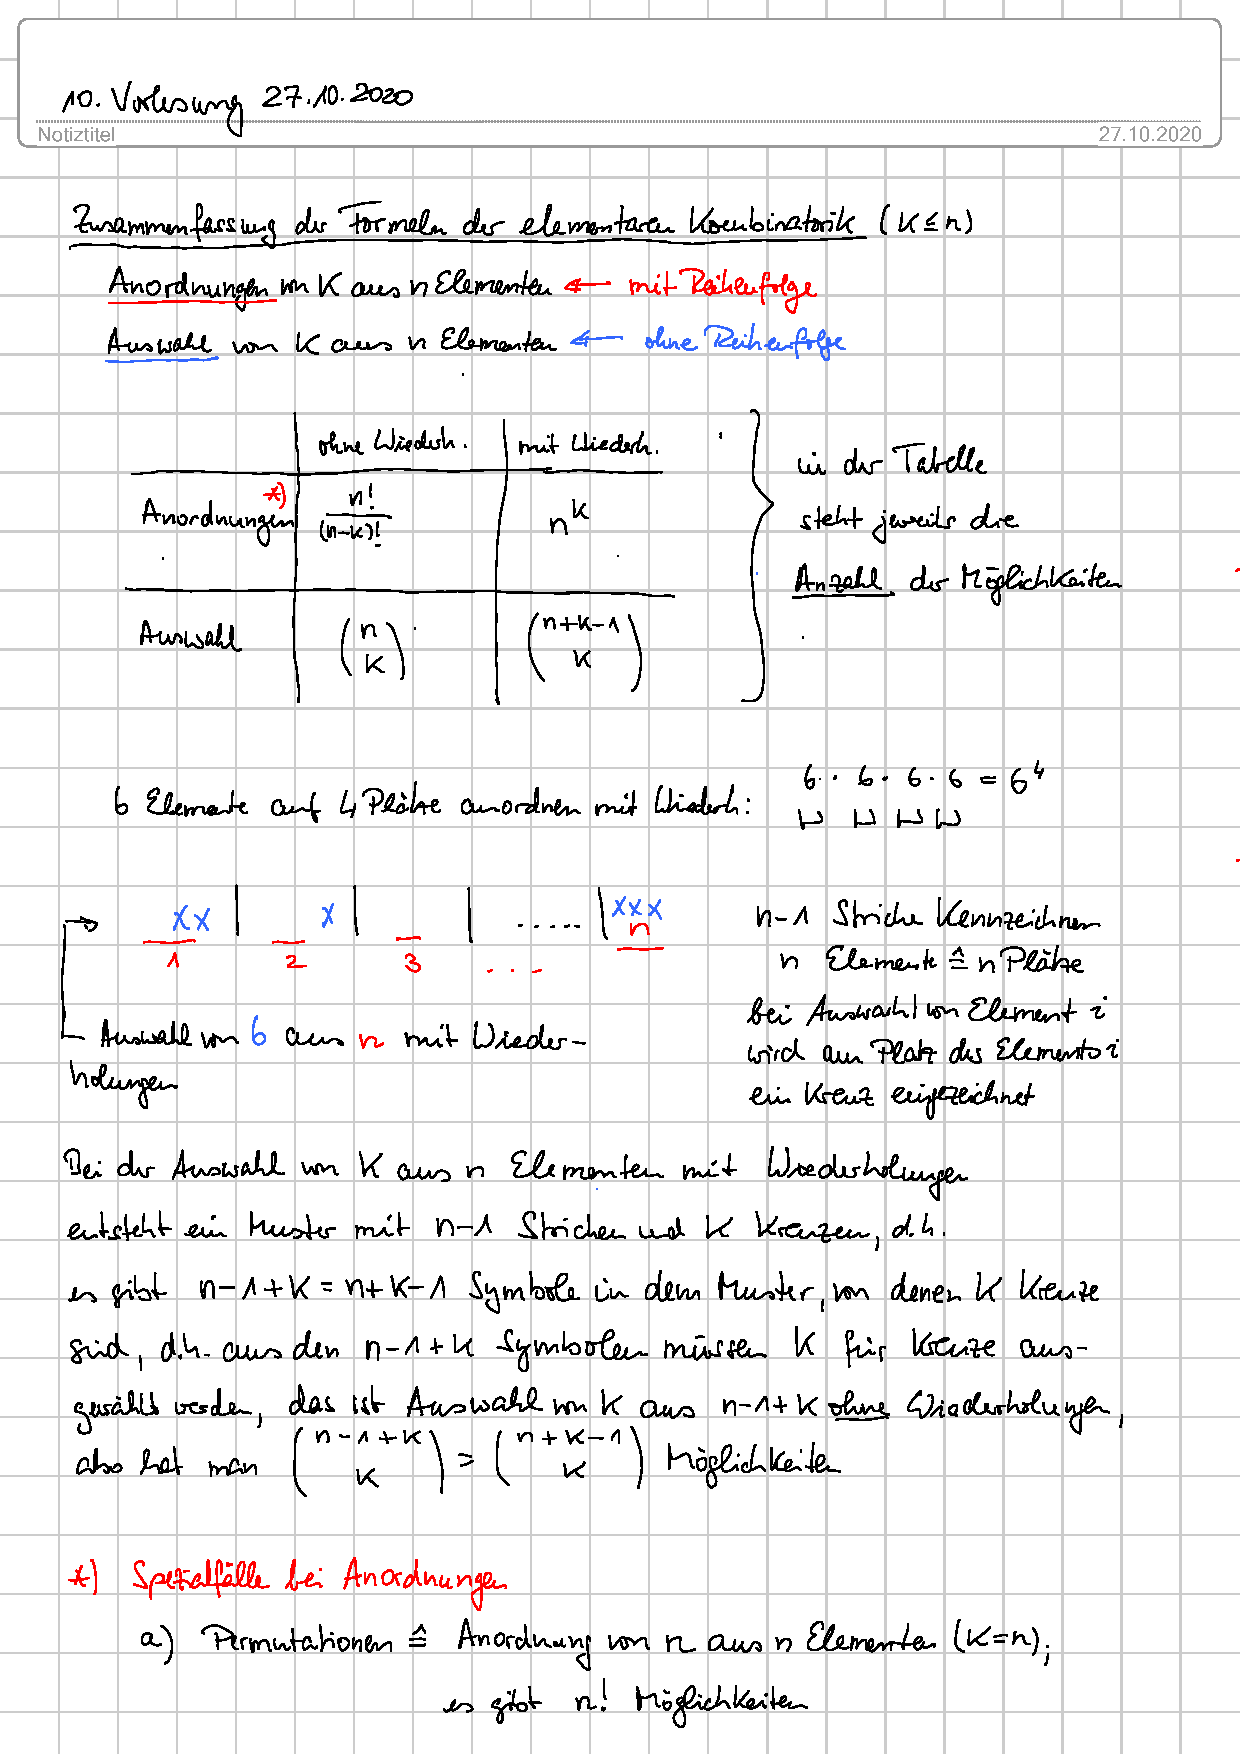
\includepdf[pages=-]{Mitschriften/10. Vorlesung 27.10.2020}

\section{Vorlesung 11 (28.10.2020)}
\subsection{Rechenregeln der Anordnung}
\subsection{Intervalle als Mengen}
\subsection{unendlich-Symbol}
\subsection{Definition: Term}
\subsection{Definition: Betrag einer reellen Zahl}
\subsection{erste Rechenregeln für den Betrag}
\subsection{Betrag, Ungleichung und Intervalle}
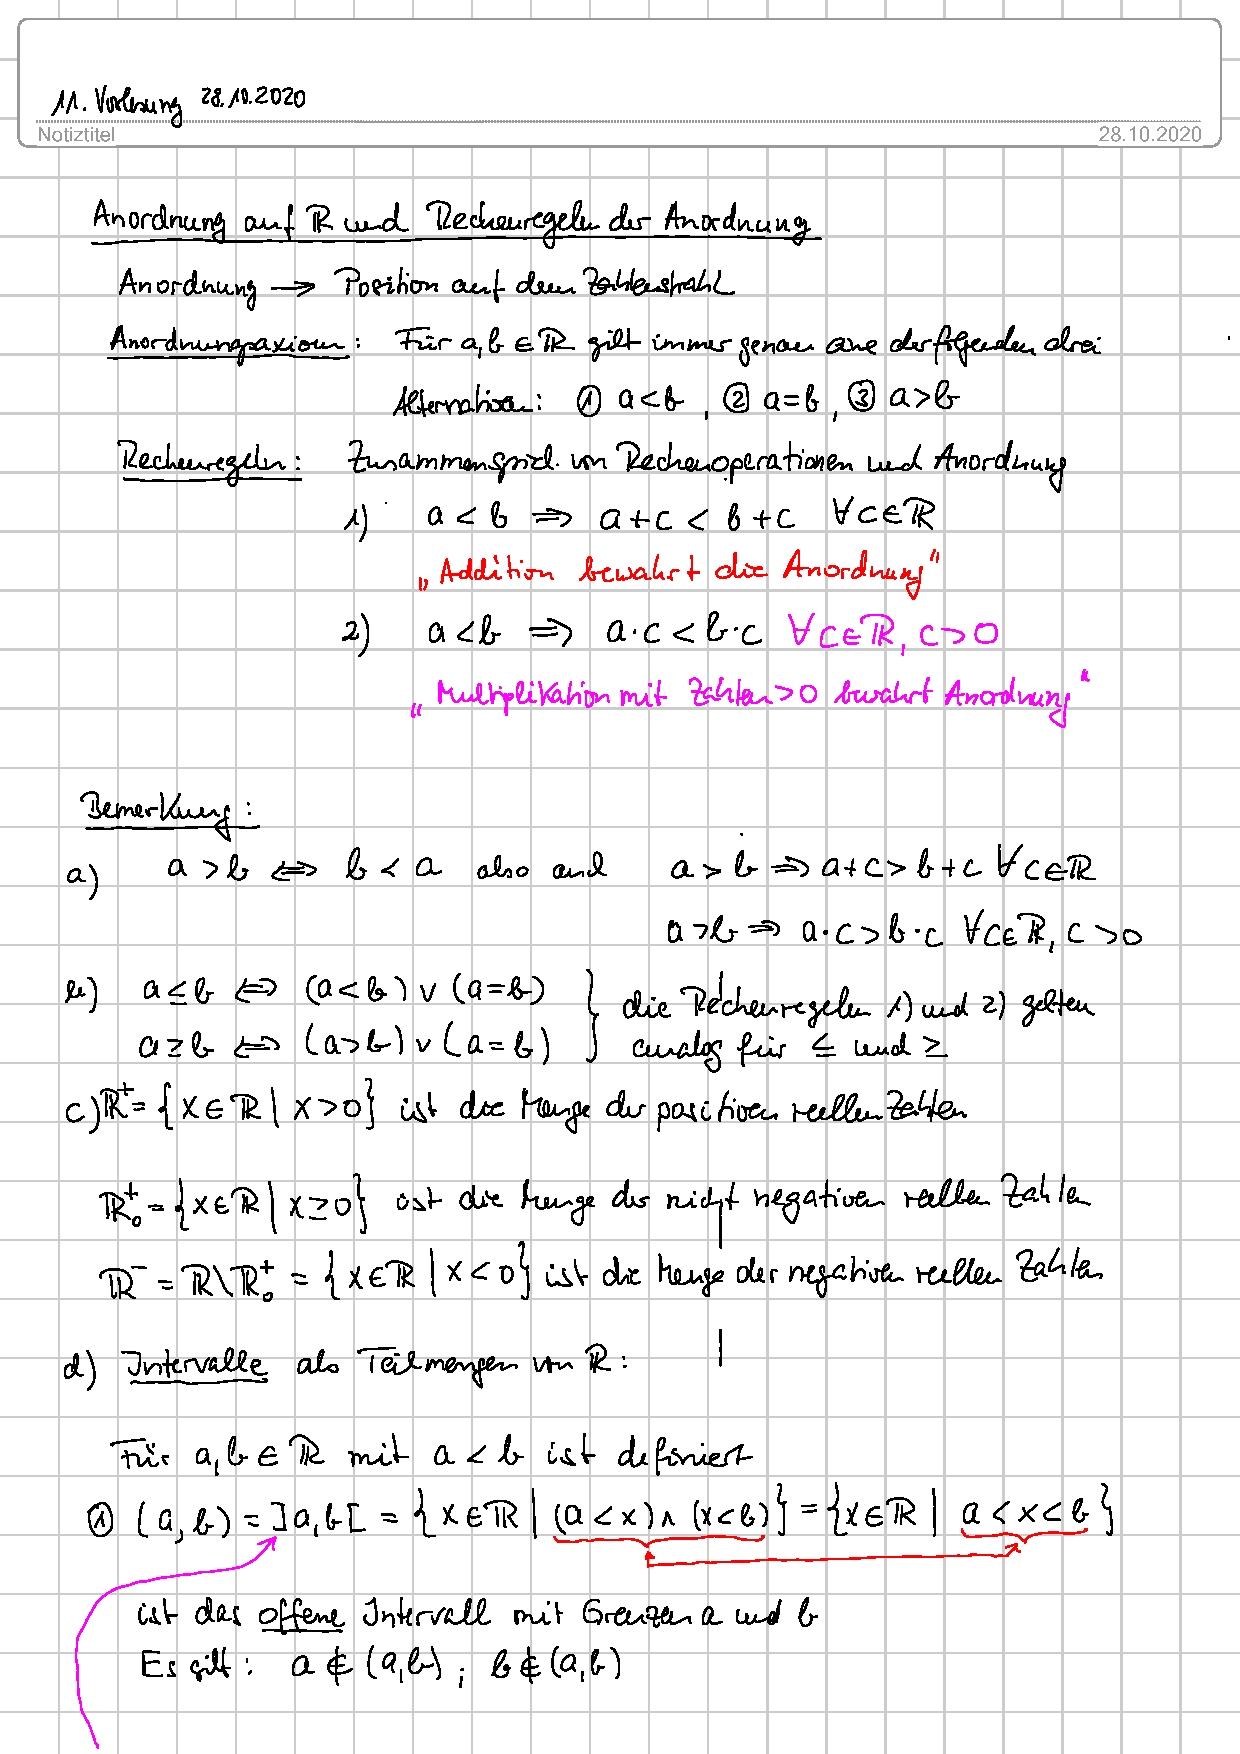
\includepdf[pages=-]{Mitschriften/11. Vorlesung 28.10.2020}

\section{Vorlesung 12 (02.11.2020)}
\subsection{Anordnung, Ungleichung und Intervalle}
\subsection{Potenzen und Wurzeln in den reellen Zahlen}
\subsection{Rechenregeln für Wurzeln}
\subsection{Quadratische Gleichungen und Ungleichungen in den reellen Zahlen}
\subsection{pq-Formel}
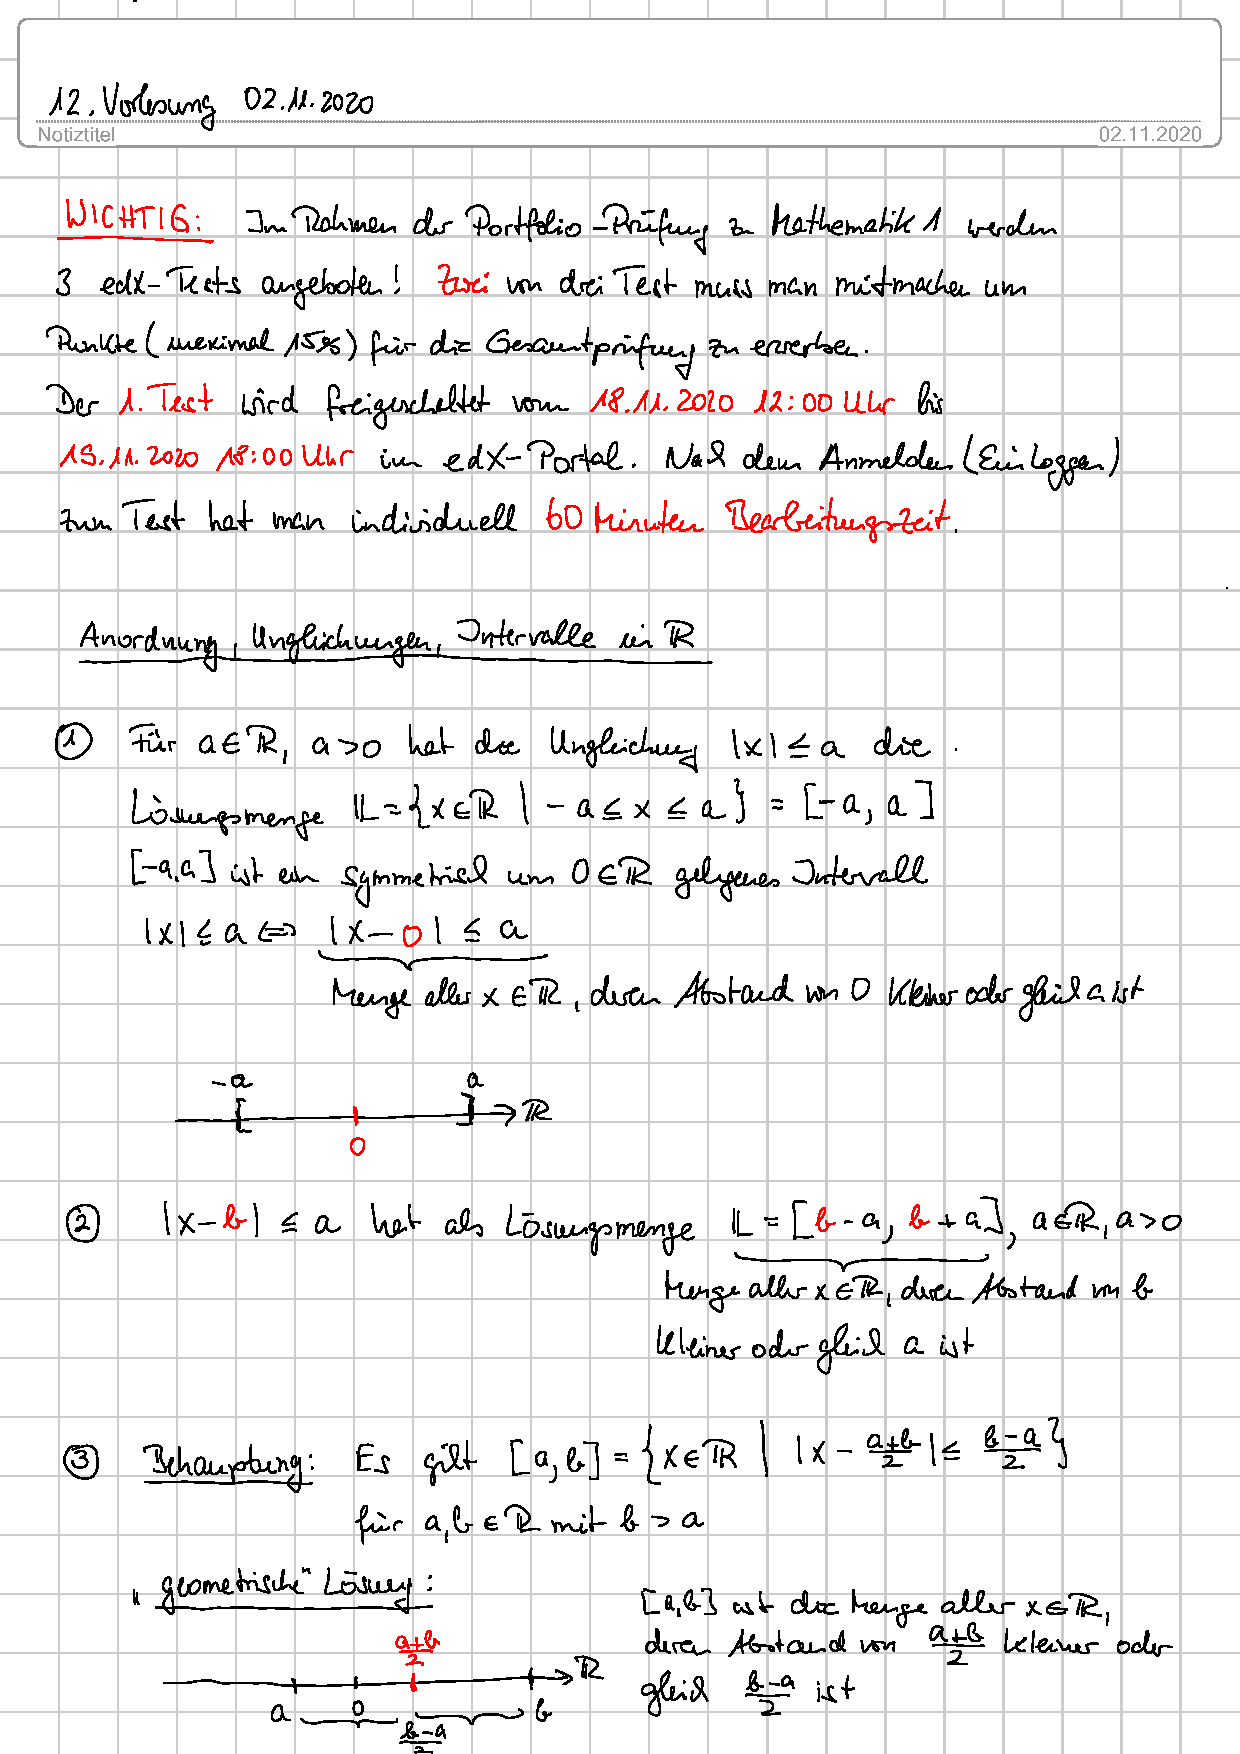
\includepdf[pages=-]{Mitschriften/12. Vorlesung 02.11.2020}

\section{Vorlesung 13 (03.11.2020)}
\subsection{Linearfaktoren des quadratischen Polynoms}
\subsection{Mitternachtsformel}
\subsection{Quadratische Ungleichungen}
\subsection{Definition: Logarithmus}
\subsection{Rechenregeln für Logarithmen}
\subsection{Zahldarstellungen (umrechnung)}
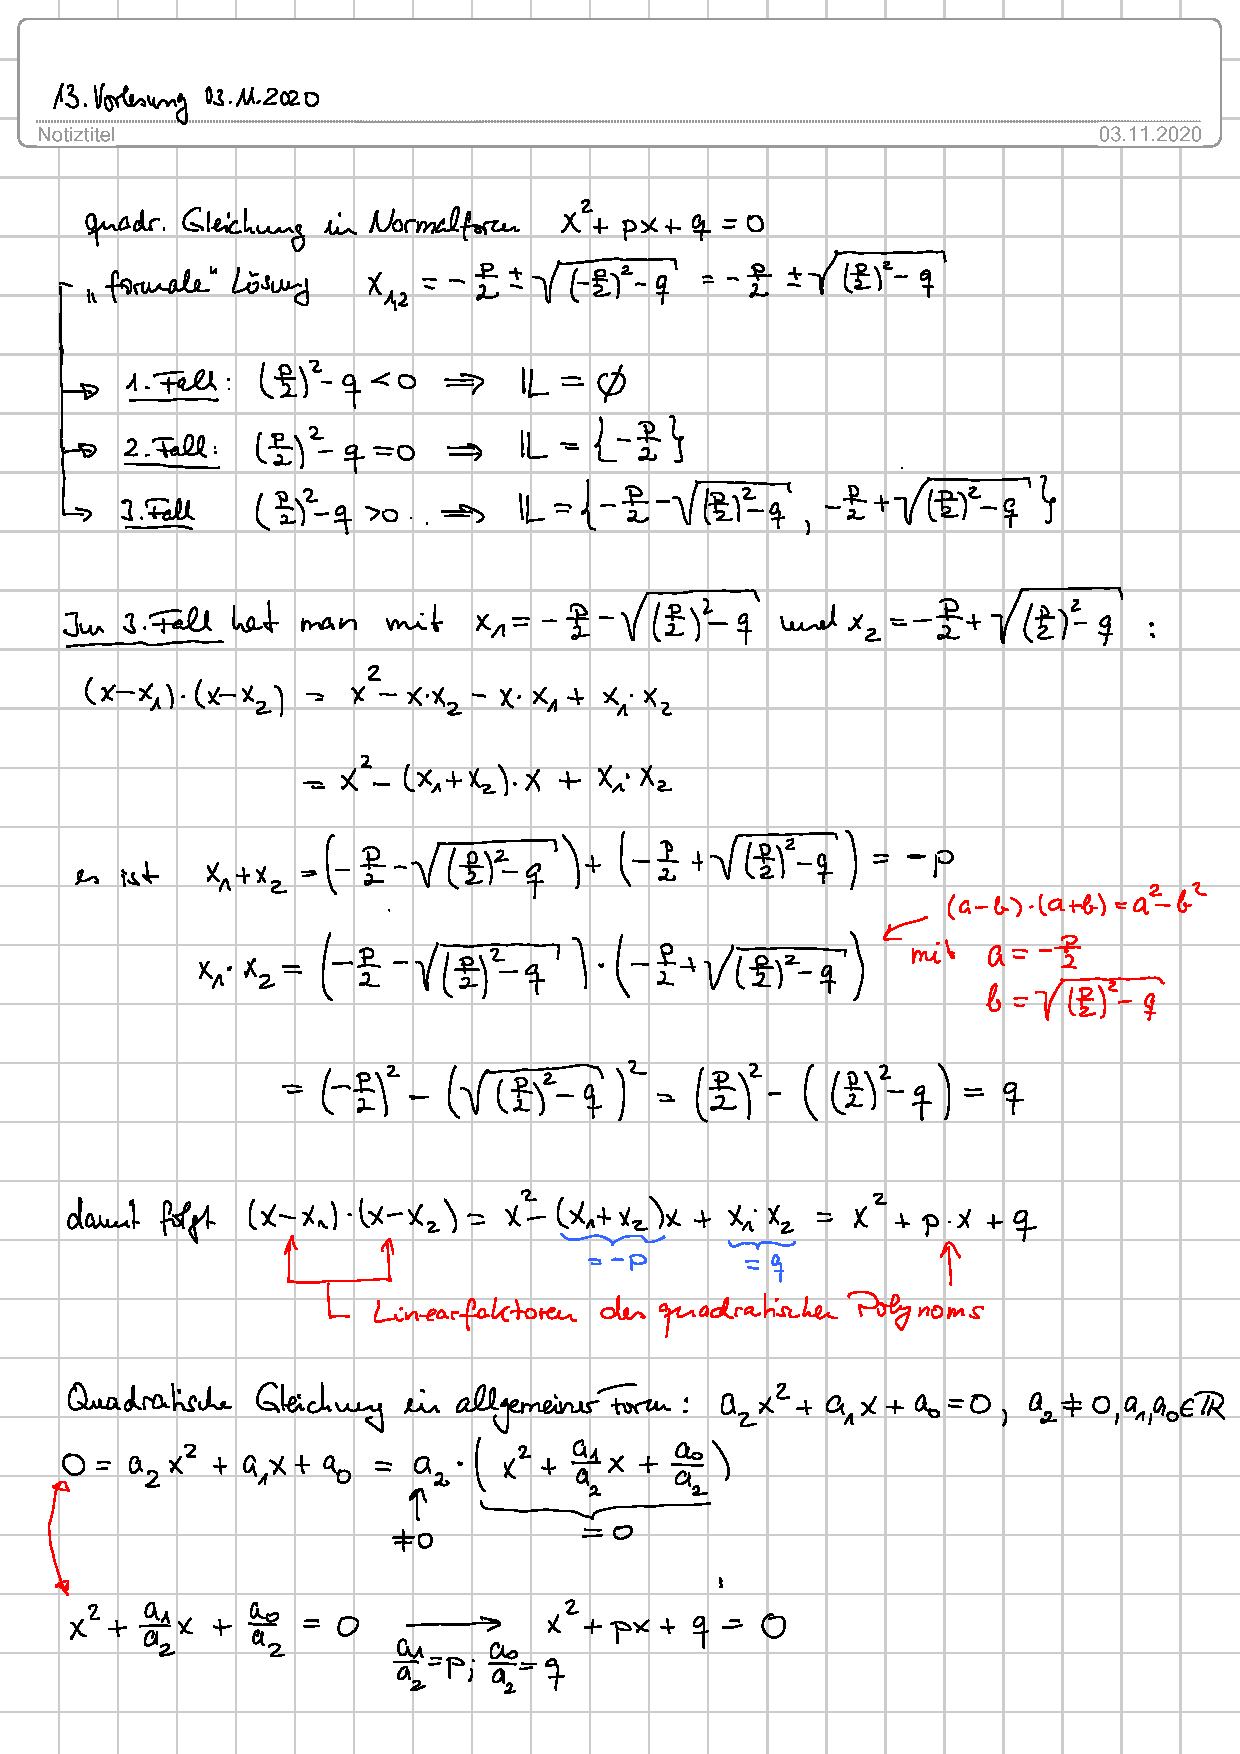
\includepdf[pages=-]{Mitschriften/13. Vorlesung 03.11.2020}

\section{Vorlesung 14 (04.11.2020)}
\subsection{Beispiel: Zahldarstellungen (umrechnung)}
\subsection{Brüche in anderen Zahldarstellungen}
\subsection{Zweiter Blick auf Ungleichungen und Betrag}
\subsection{Rechenregeln für den Betrag}
\subsection{Beweisidee Dreiecksungleichung}
\subsection{Definition: Verknüfungen auf Mengen}
\subsection{Definition: Gruppe, Halbgruppe, abelsche Gruppe}
\subsection{Definition: Ring, Ring mit Eins, Kommutativer Ring mit Eins}
\subsection{Definition: Körper}
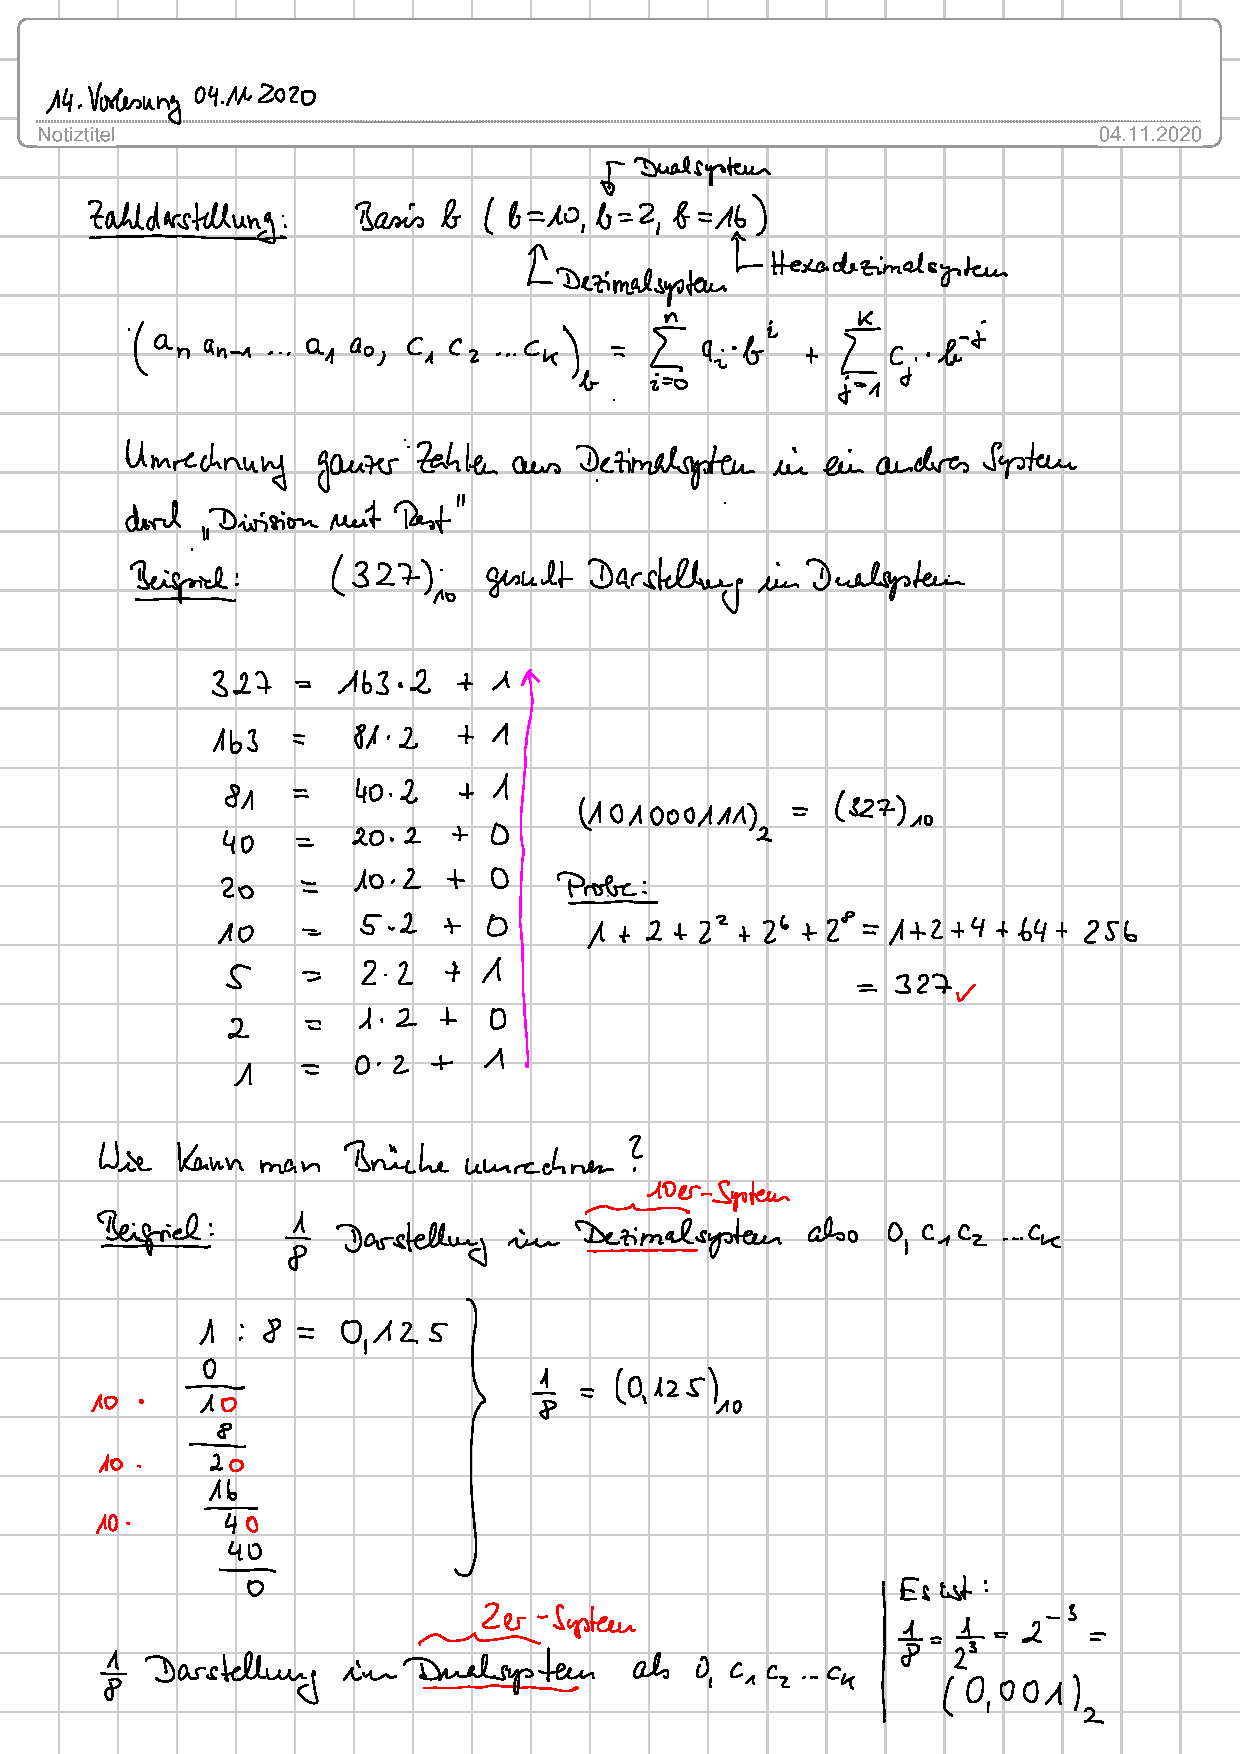
\includepdf[pages=-]{Mitschriften/14. Vorlesung 04.11.2020}

\section{Vorlesung 15 (16.11.2020)}
\subsection{5 Körperaxiome + Beispiele}
\subsection{Definition: Ganzzahlige Teiler}
\subsection{Definition: Primzahl}
\subsection{Definition: Gemeinsame Teiler / Größter gemeinsamer Teiler}
\subsection{Division mit Rest}
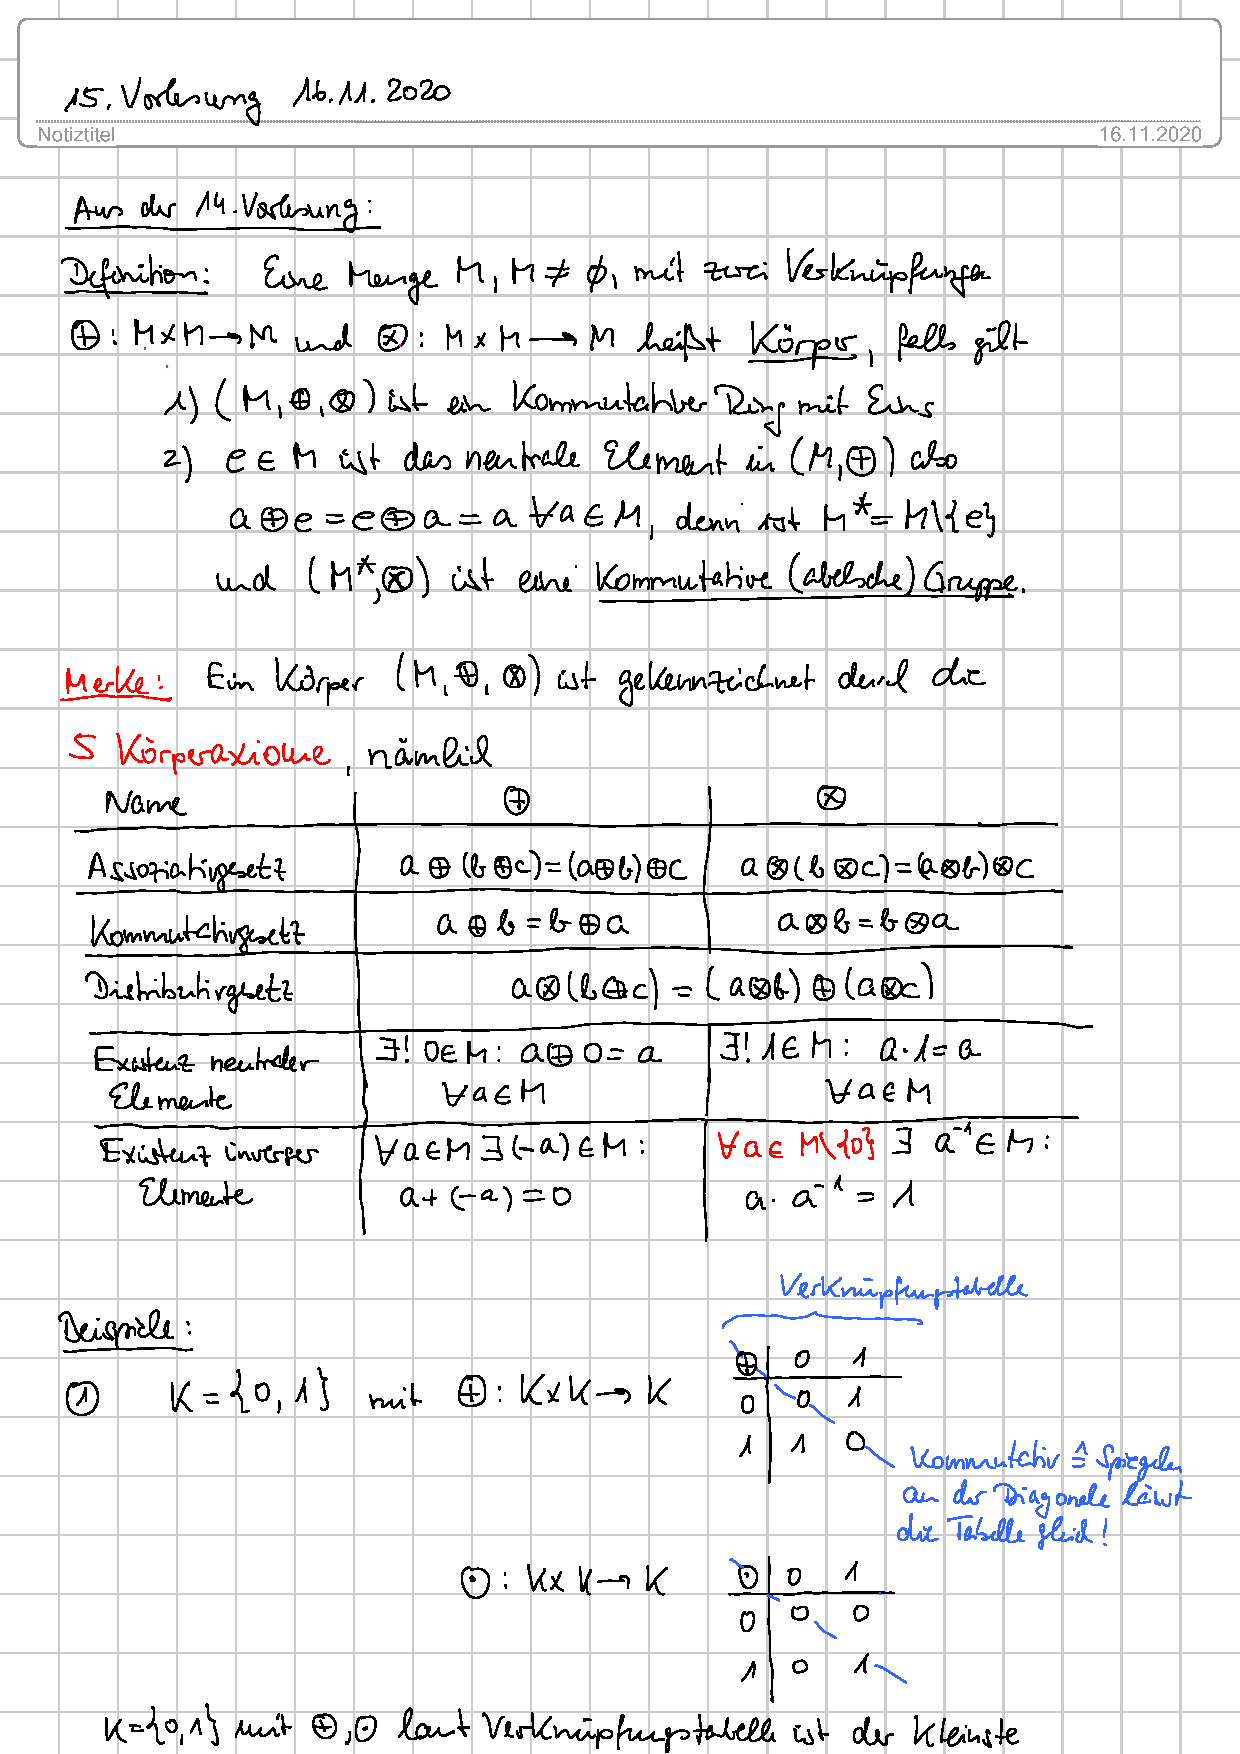
\includepdf[pages=-]{Mitschriften/15. Vorlesung 16.11.2020}

\section{Vorlesung 16 (17.11.2020)}
\subsection{Wiederholung Teilermengen, Primzahl, gemeinsame Teiler}
\subsection{Definition: ggT, Division mit Rest, Teilerfremd}
\subsection{Beweis: Division mit Rest}
\subsection{Euklidischer Algorithmus}
\subsection{Lemma von Bézout}
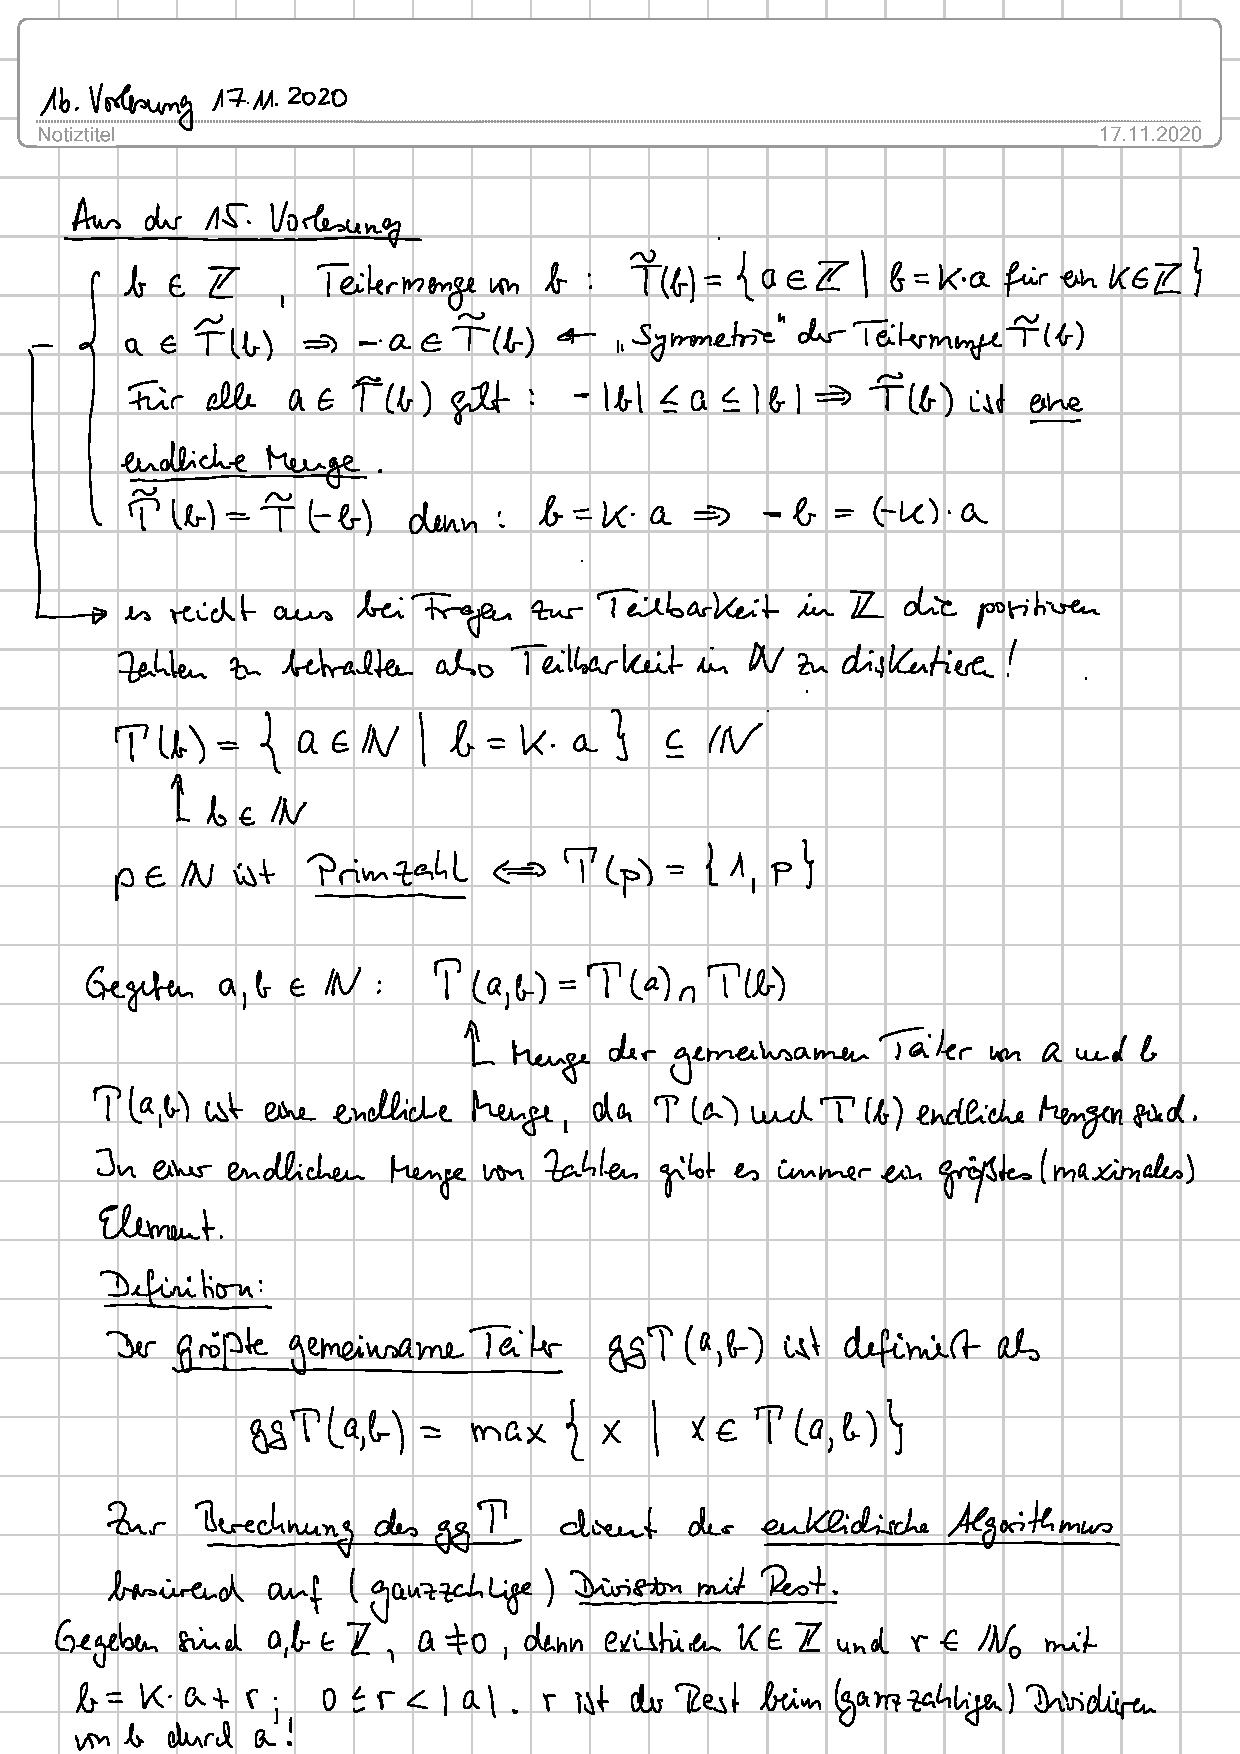
\includepdf[pages=-]{Mitschriften/16. Vorlesung 17.11.2020}


\section{Vorlesung 17 (18.11.2020)}
\subsection{Teilen mit Rest}
\subsection{Teilen und Äquivalenzrelationen, Restemengen}
\subsection{Rechenoperationen in $Z_m$, Körper?, kommutativer Ring mit Eins?}
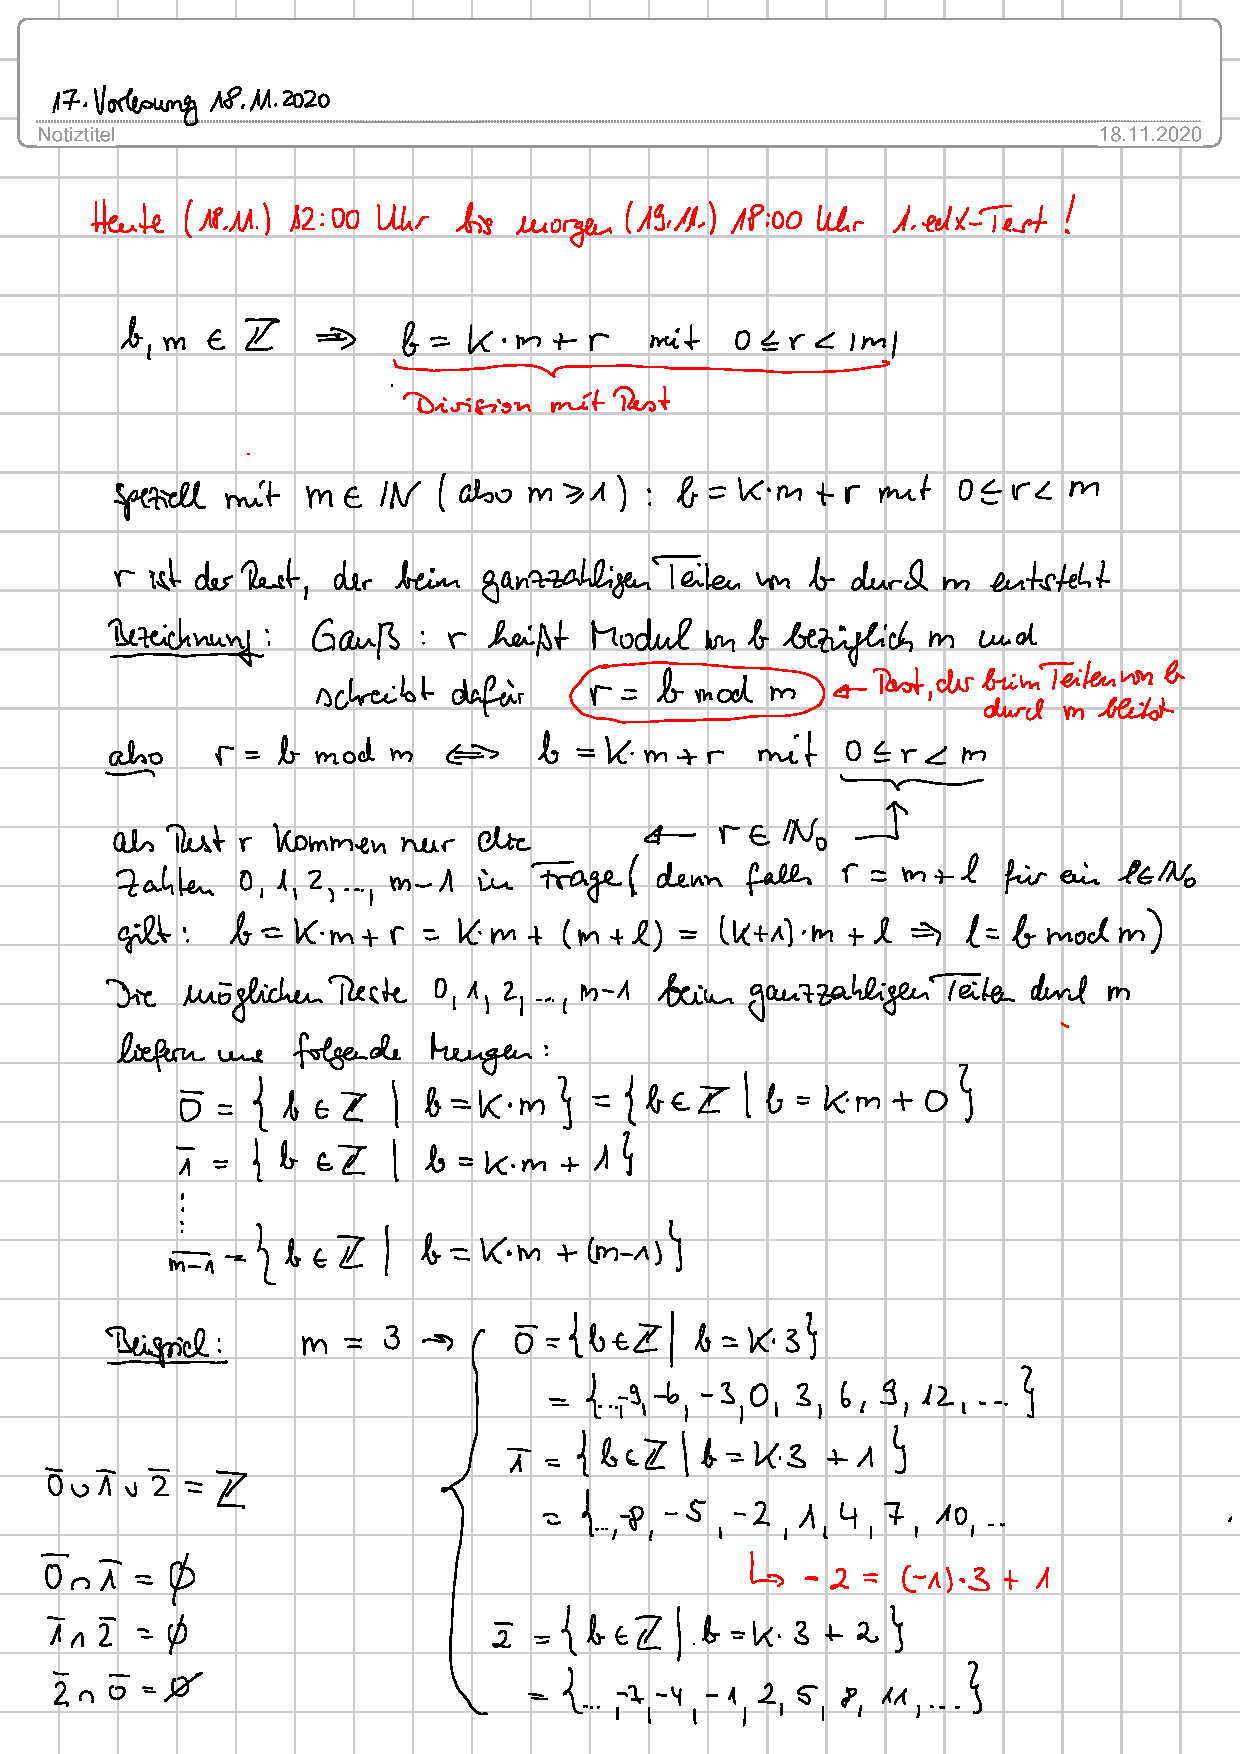
\includepdf[pages=-]{Mitschriften/17. Vorlesung 18.11.2020}

\section{Vorlesung 18 (23.11.2020)}
\subsection{Restklassen mit Primzahlen sind Körper + Beispiel}
\subsection{simultane Kongruenzen}
\subsection{chinesischer Restsatz}
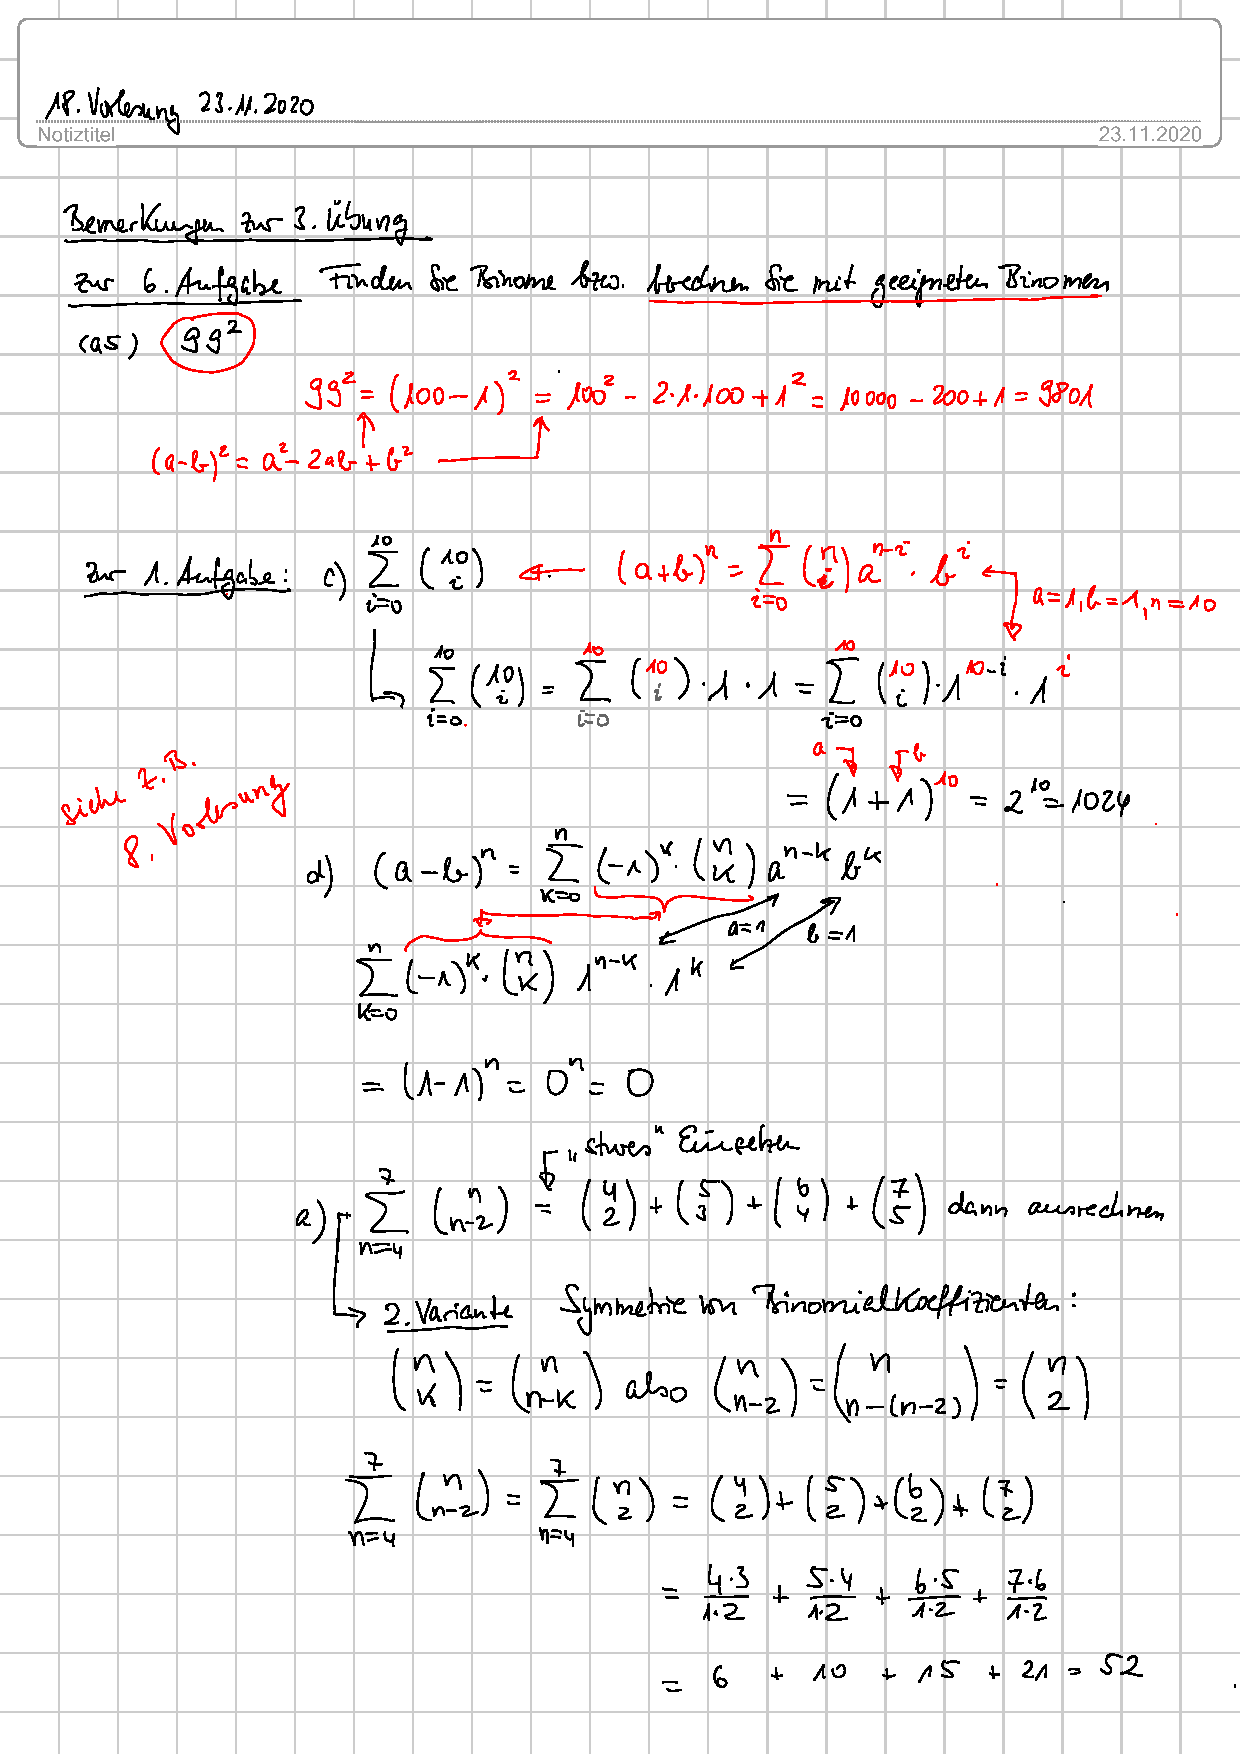
\includepdf[pages=-]{Mitschriften/18. Vorlesung 23.11.2020}

\section{Vorlesung 19 (24.11.2020)}
\subsection{Chinesischer Restsatz: Beweis, Beispiel}
\subsection{Allgemeiner chinesischer Restsatz}
\subsection{RSA: Anwendung von modularer Arithmetik}
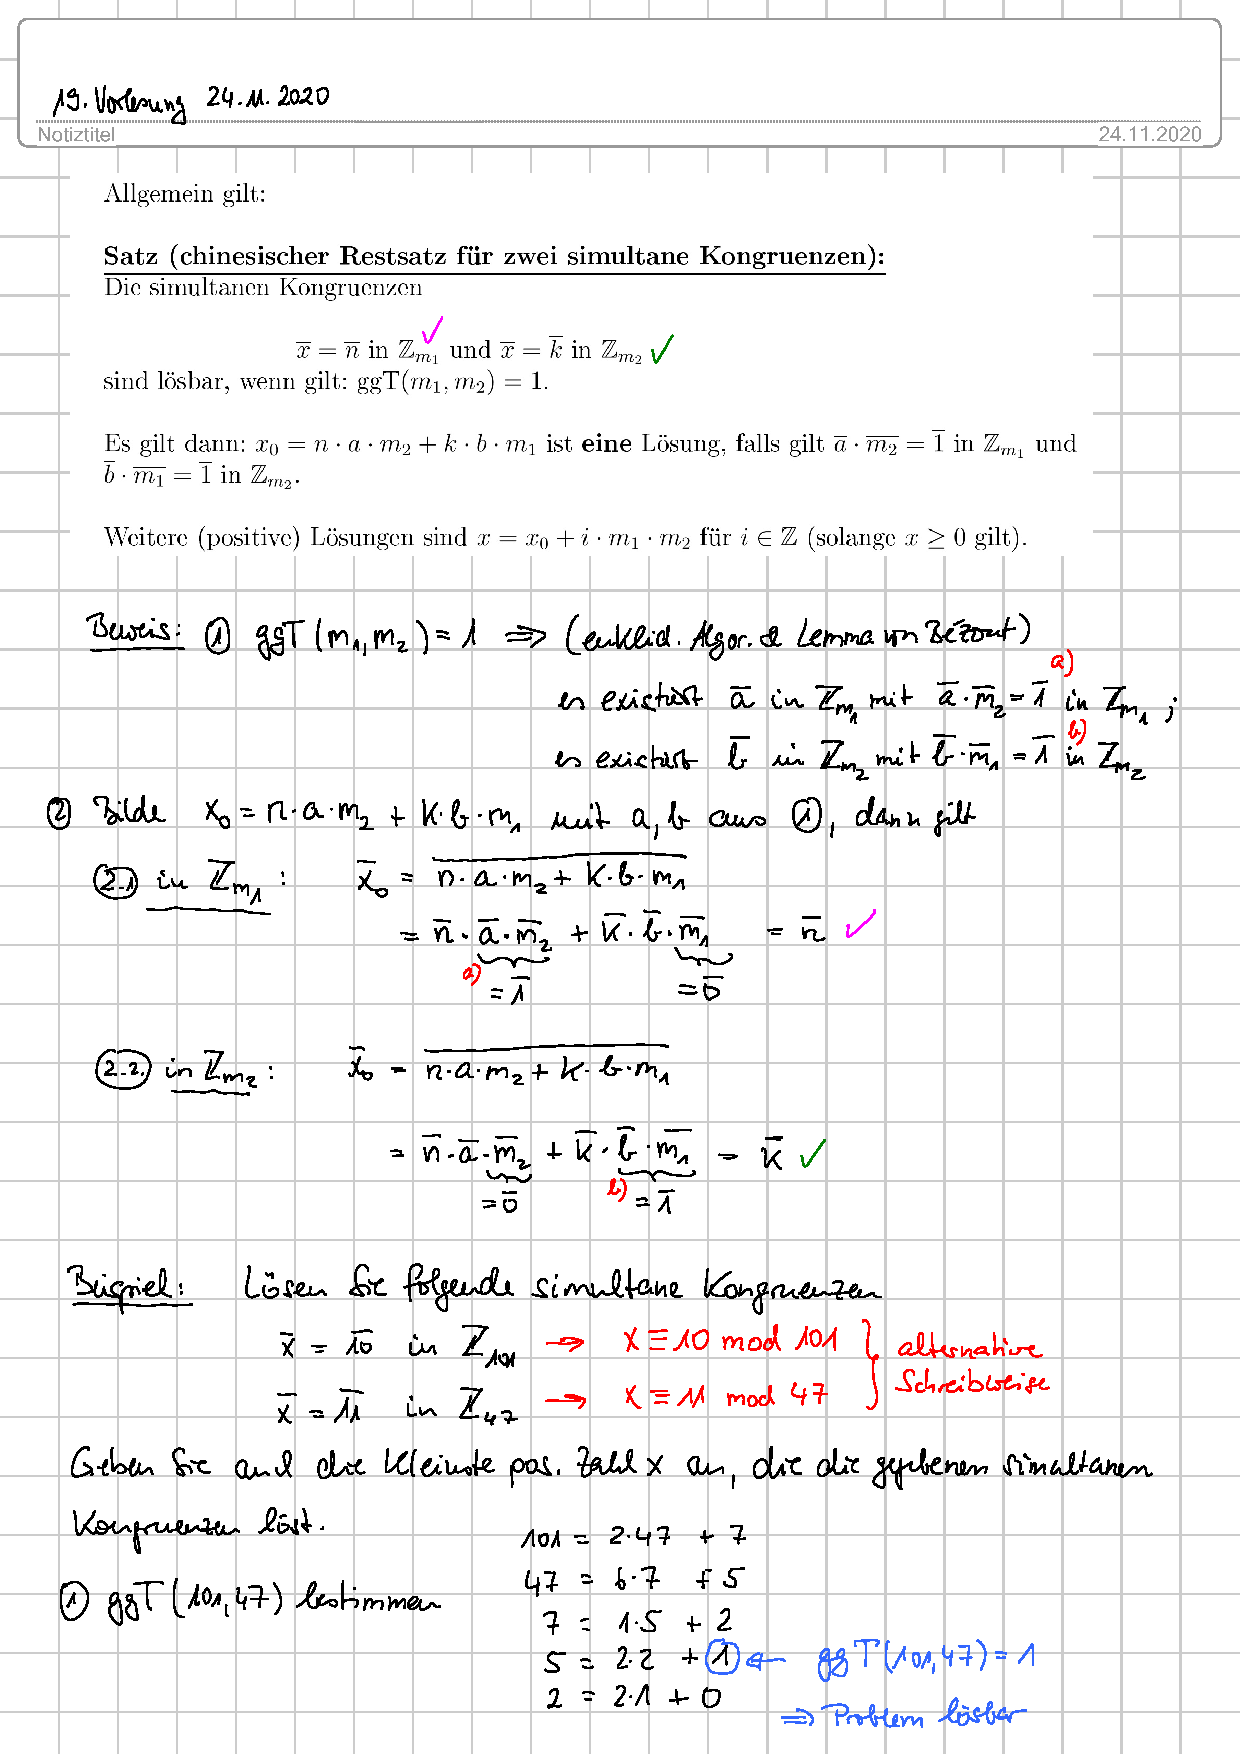
\includepdf[pages=-]{Mitschriften/19. Vorlesung 24.11.2020}

\section{Vorlesung 20 (25.11.2020)}
\subsection{Prinzip der RSA-Verschlüsselung}
\subsection{Eulersche-phi-Funktion}
\subsection{Satz von Euler}
\subsection{'kleiner' Satz von Fermat}
\subsection{Beweis: RSA-Algorithmus}
\subsection{Beweis: Satz von Euler}
\subsection{Einführung: Lineare Gleichungssysteme}
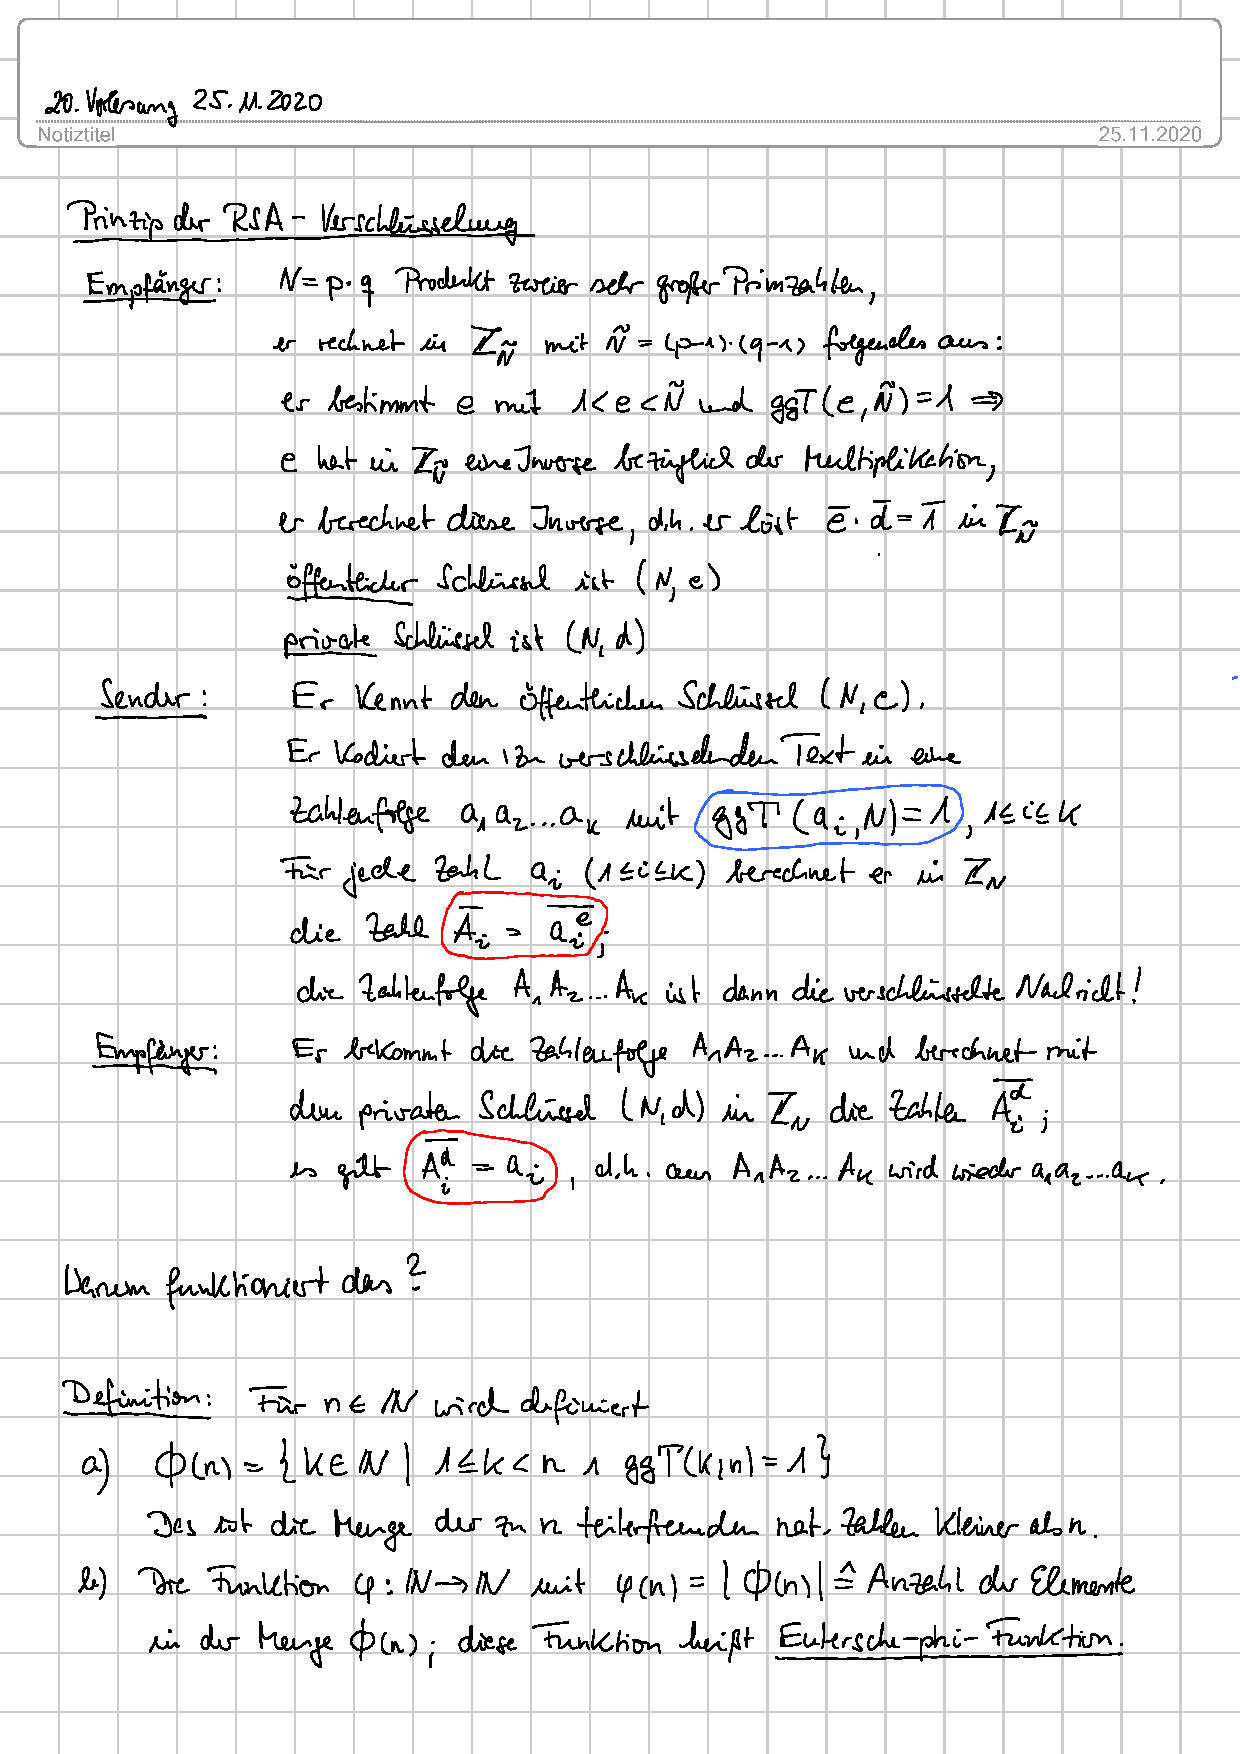
\includepdf[pages=-]{Mitschriften/20. Vorlesung 25.11.2020}

\section{Vorlesung 21 (30.11.2020)}
\subsection{Rechenoperationen für Vektoren}
\subsection{Definition: Linearkombination/Gewichtete Summe}
\subsection{Definition: Vektorraum}
\subsection{Einführung in Gauß-Algorithmus (Rücksubstitution)}
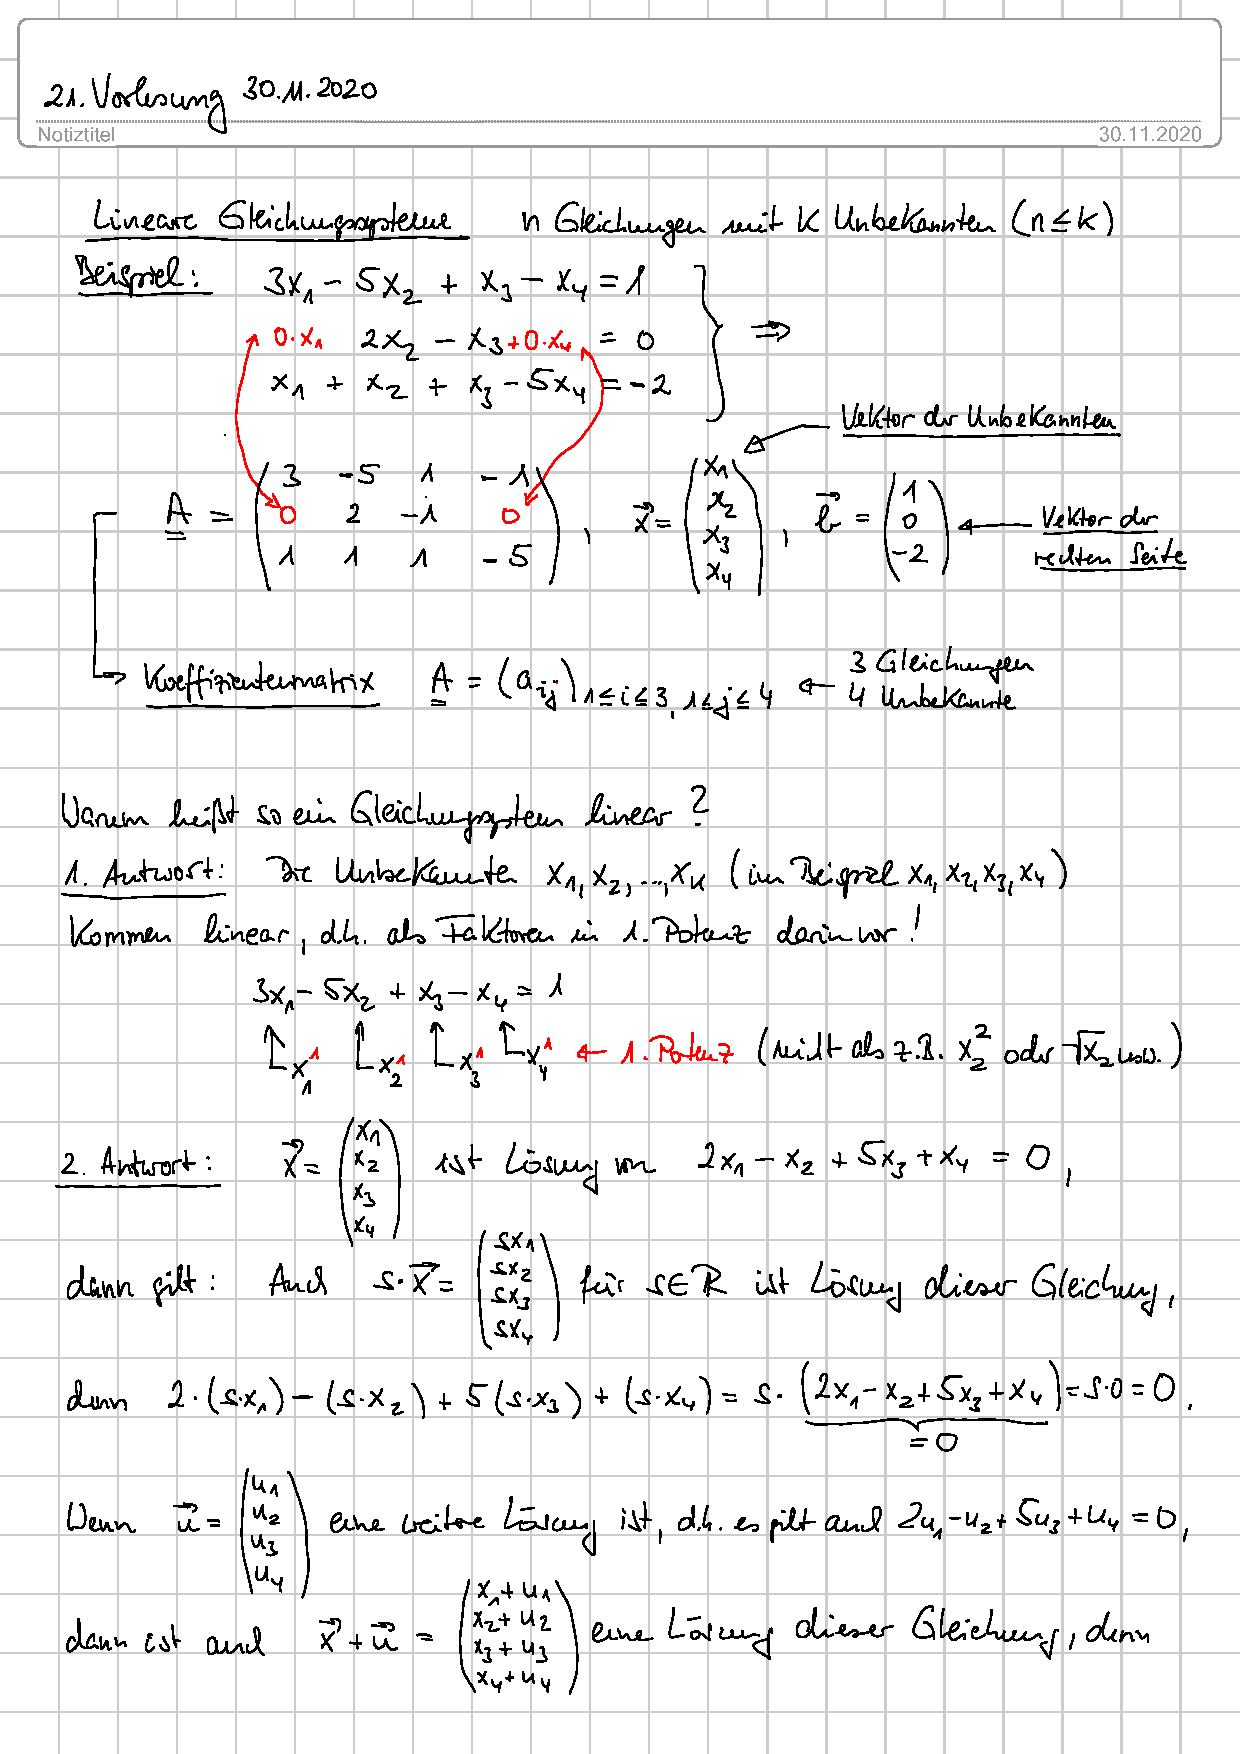
\includepdf[pages=-]{Mitschriften/21. Vorlesung 30.11.2020}

\section{Vorlesung 22 (01.12.2020)}
\subsection{Gauß-Algorithmus}
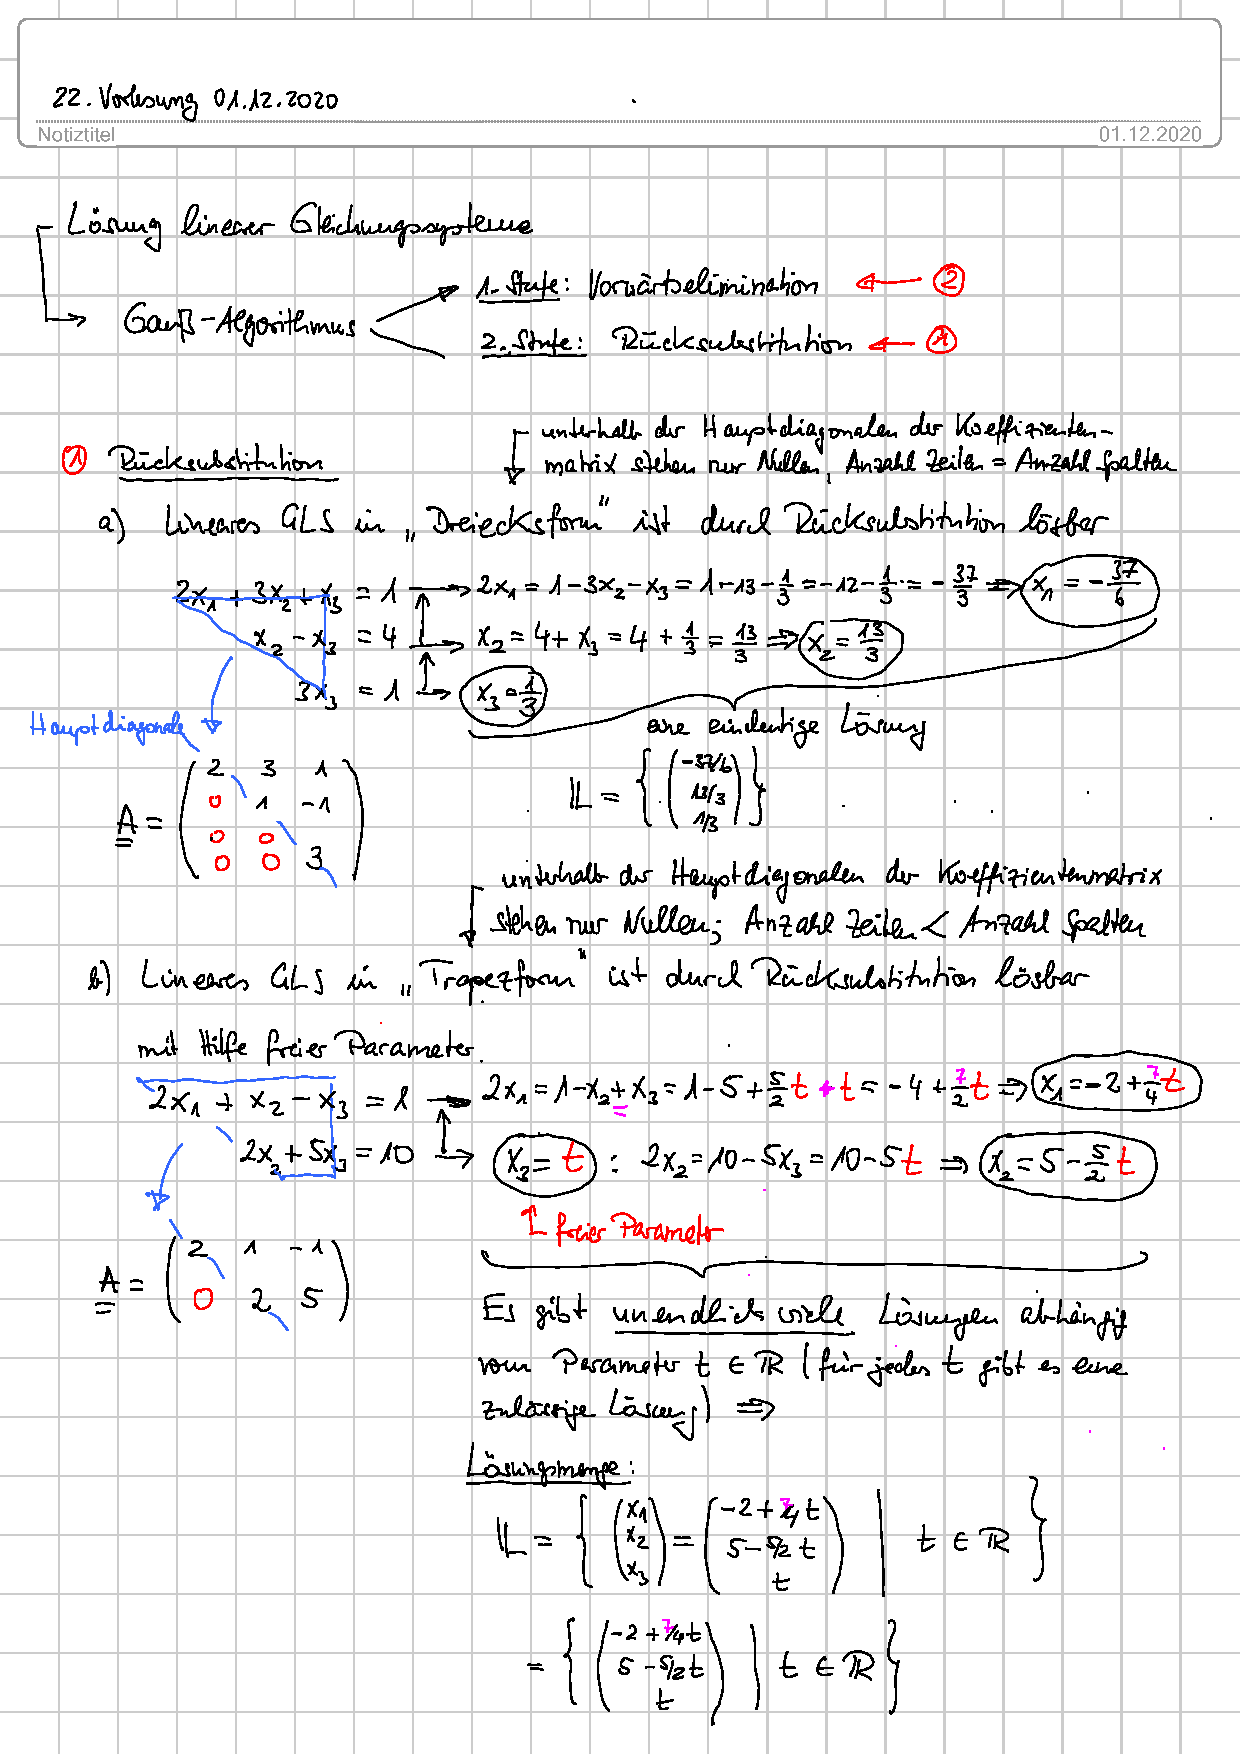
\includepdf[pages=-]{Mitschriften/22. Vorlesung 01.12.2020}

\section{Vorlesung 23 (02.12.2020)}
\subsection{Zusammenfassung lösen von LGS / Gauß-Algorithmus}
\subsection{Definition Rang von Matrizen und linearen Gleichungssystemen}
\subsection{Folgerungen aus Lösungstheorie (spezielle Lösung, allgemeine Lösung)}
\subsection{in-/homogene lineare Gleichungssysteme und deren Lösungsstruktur}
\subsection{Beispiele spezielle/allgemeine Lösungen}
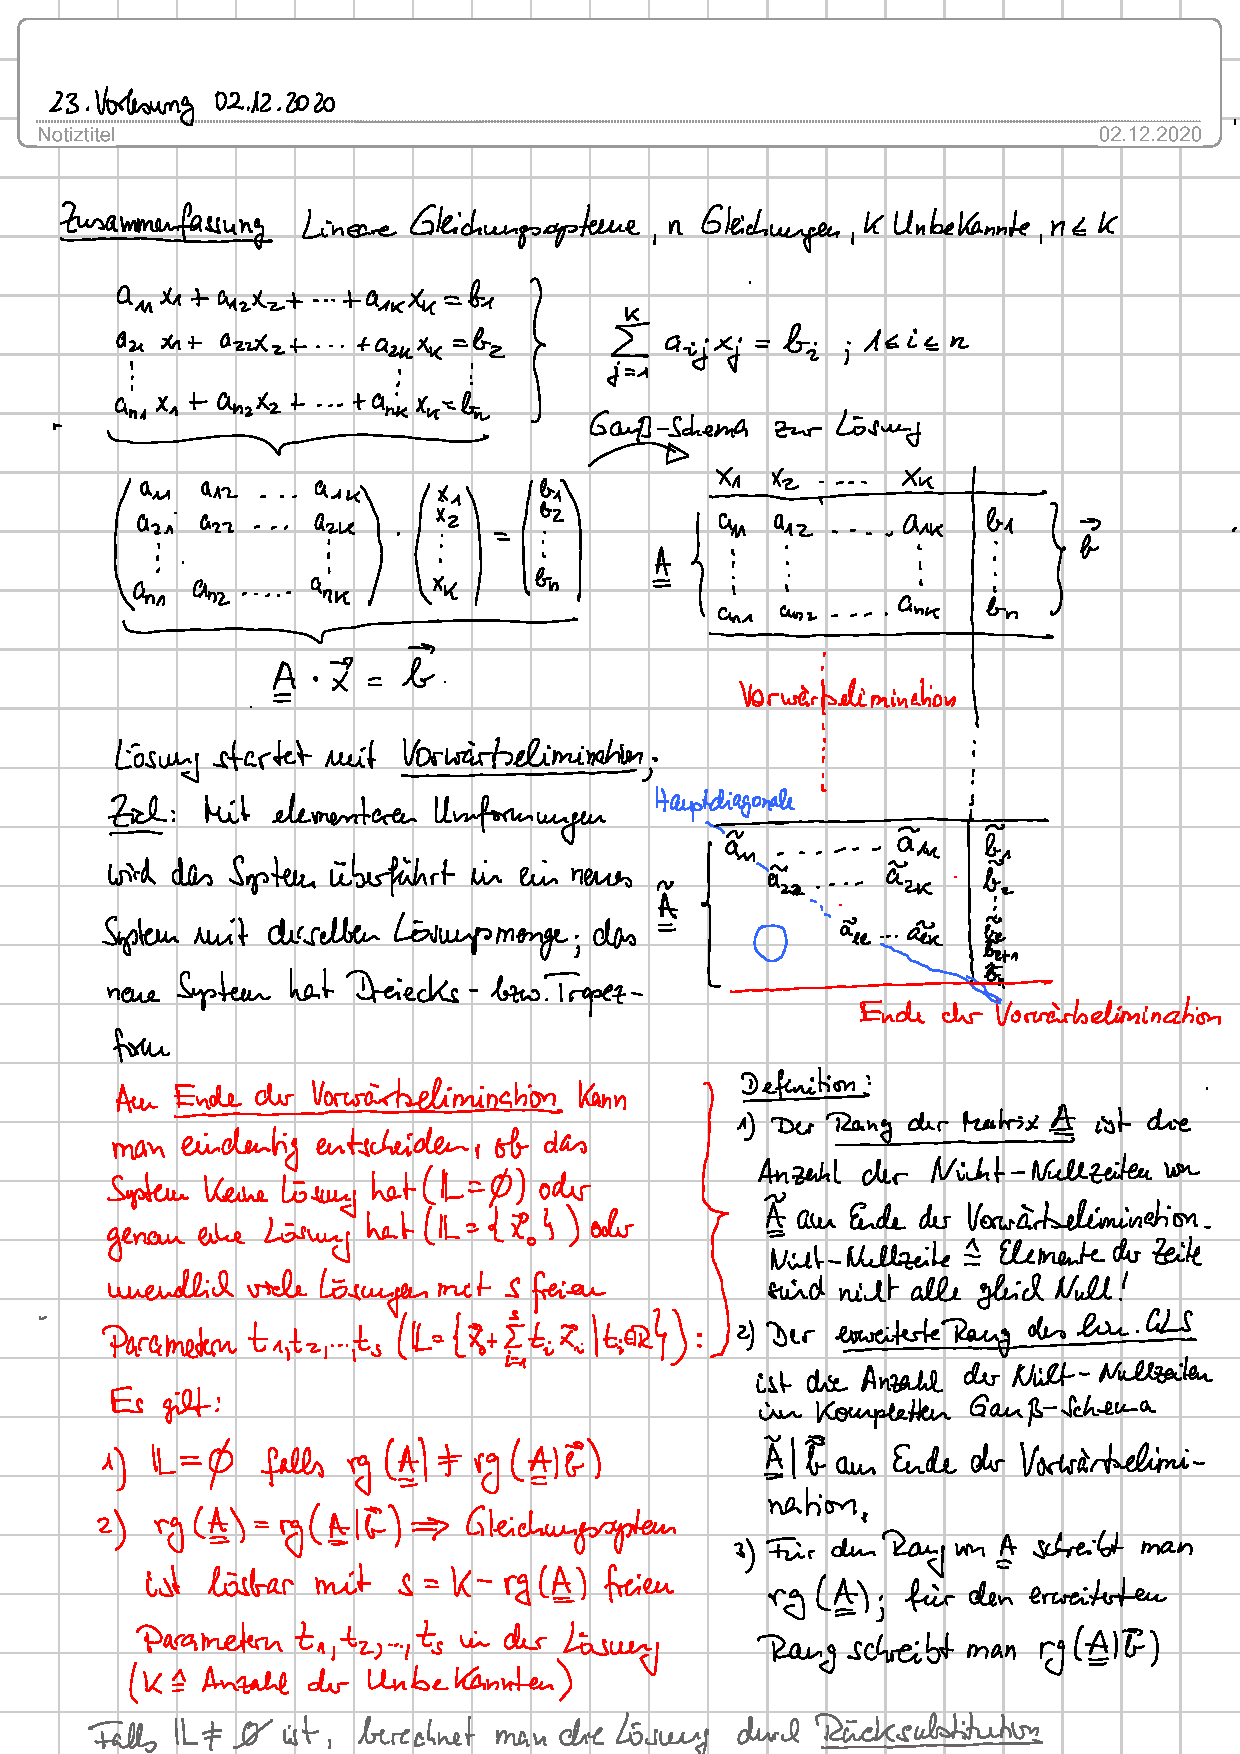
\includepdf[pages=-]{Mitschriften/23. Vorlesung 02.12.2020}


\section{Vorlesung 24 (07.12.2020)}
\subsection{Zusammenfassung LGS: Lösen, Lösungsstruktur}
\subsection{Vektoren und Vektorräume: Rechenoperationen, Pfeile}
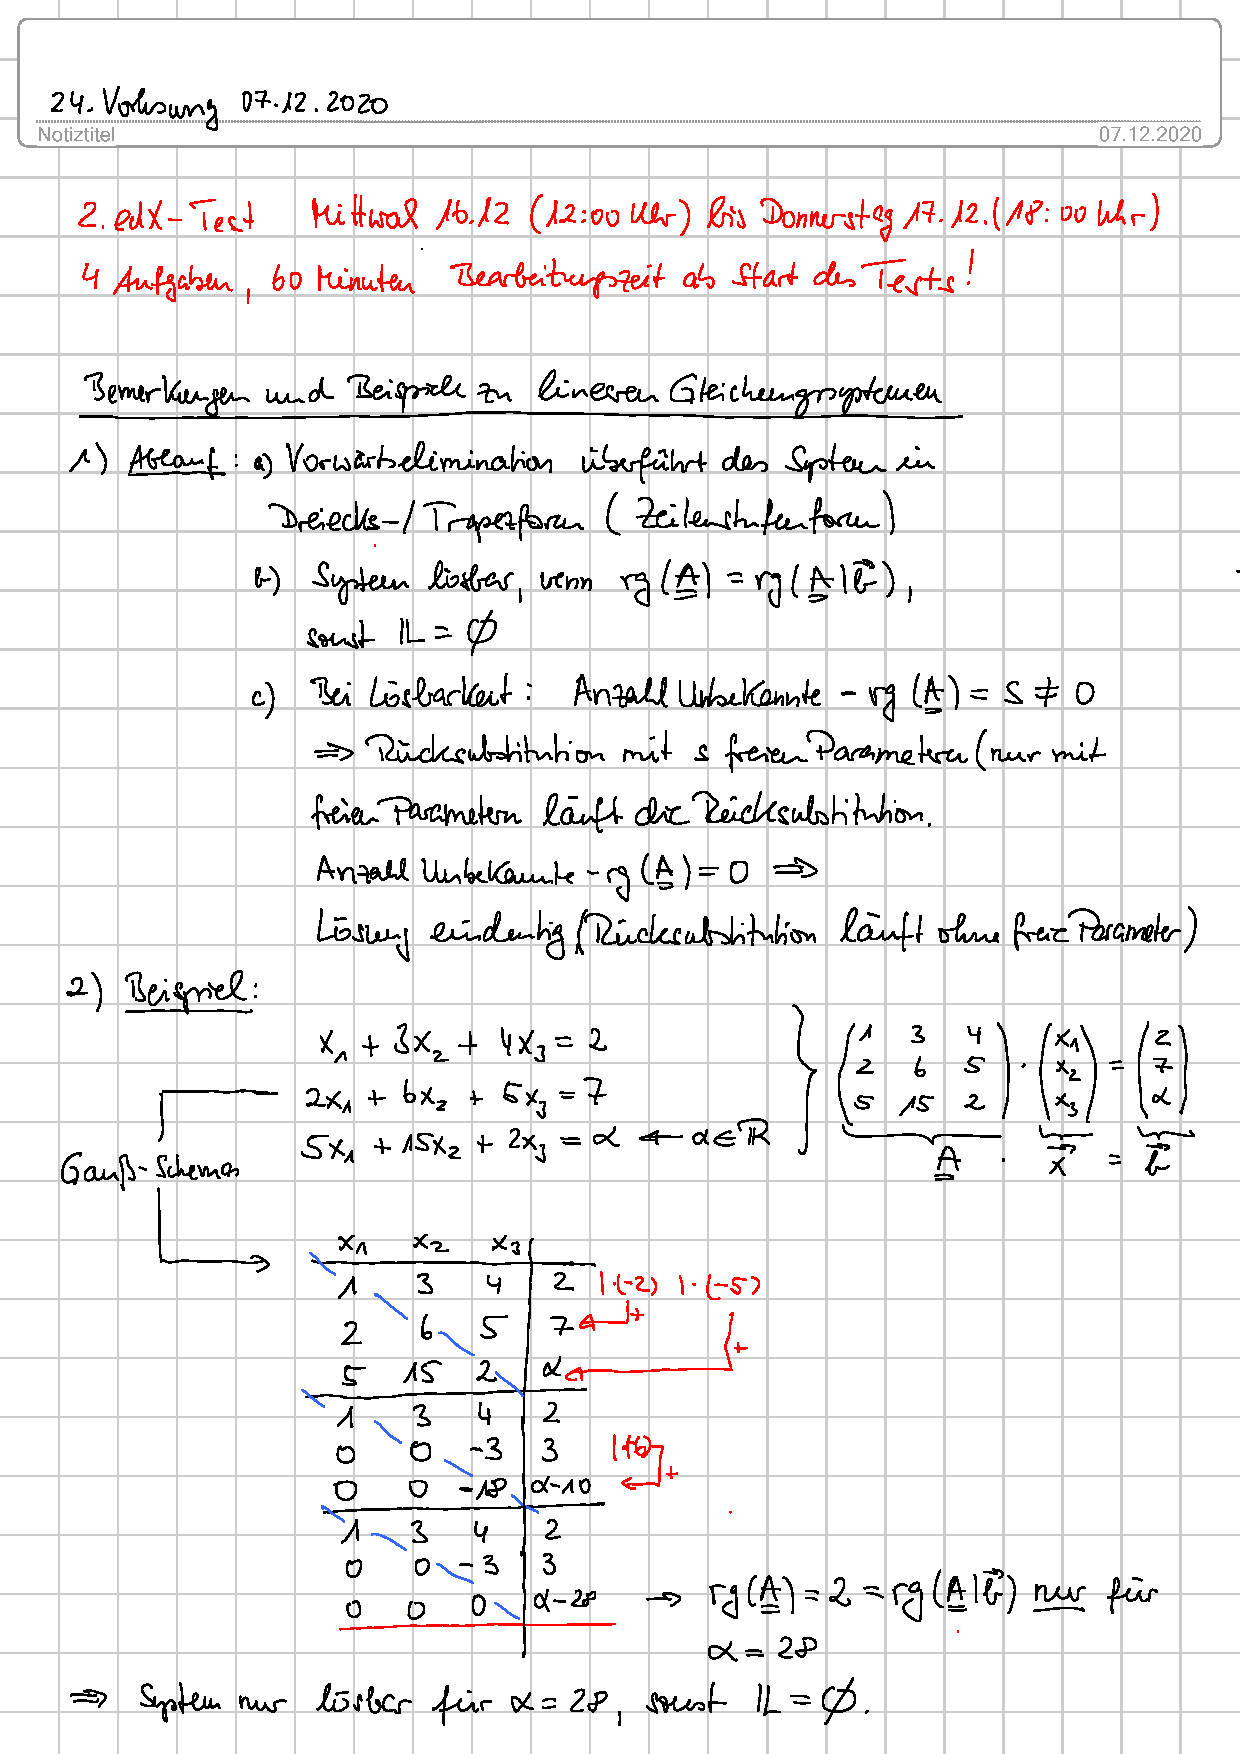
\includepdf[pages=-]{Mitschriften/24. Vorlesung 07.12.2020}

\section{Vorlesung 25 (08.12.2020)}
\subsection{Äquivalenz von Pfeilen, Punkte und Vektorsicht}
\subsection{Rechenregeln von Vektoren}
\subsection{Definition: Vektorraum}
\subsection{Definition: Erzeugendensystem, linear unabhängig, Basis eines Vektorraums}
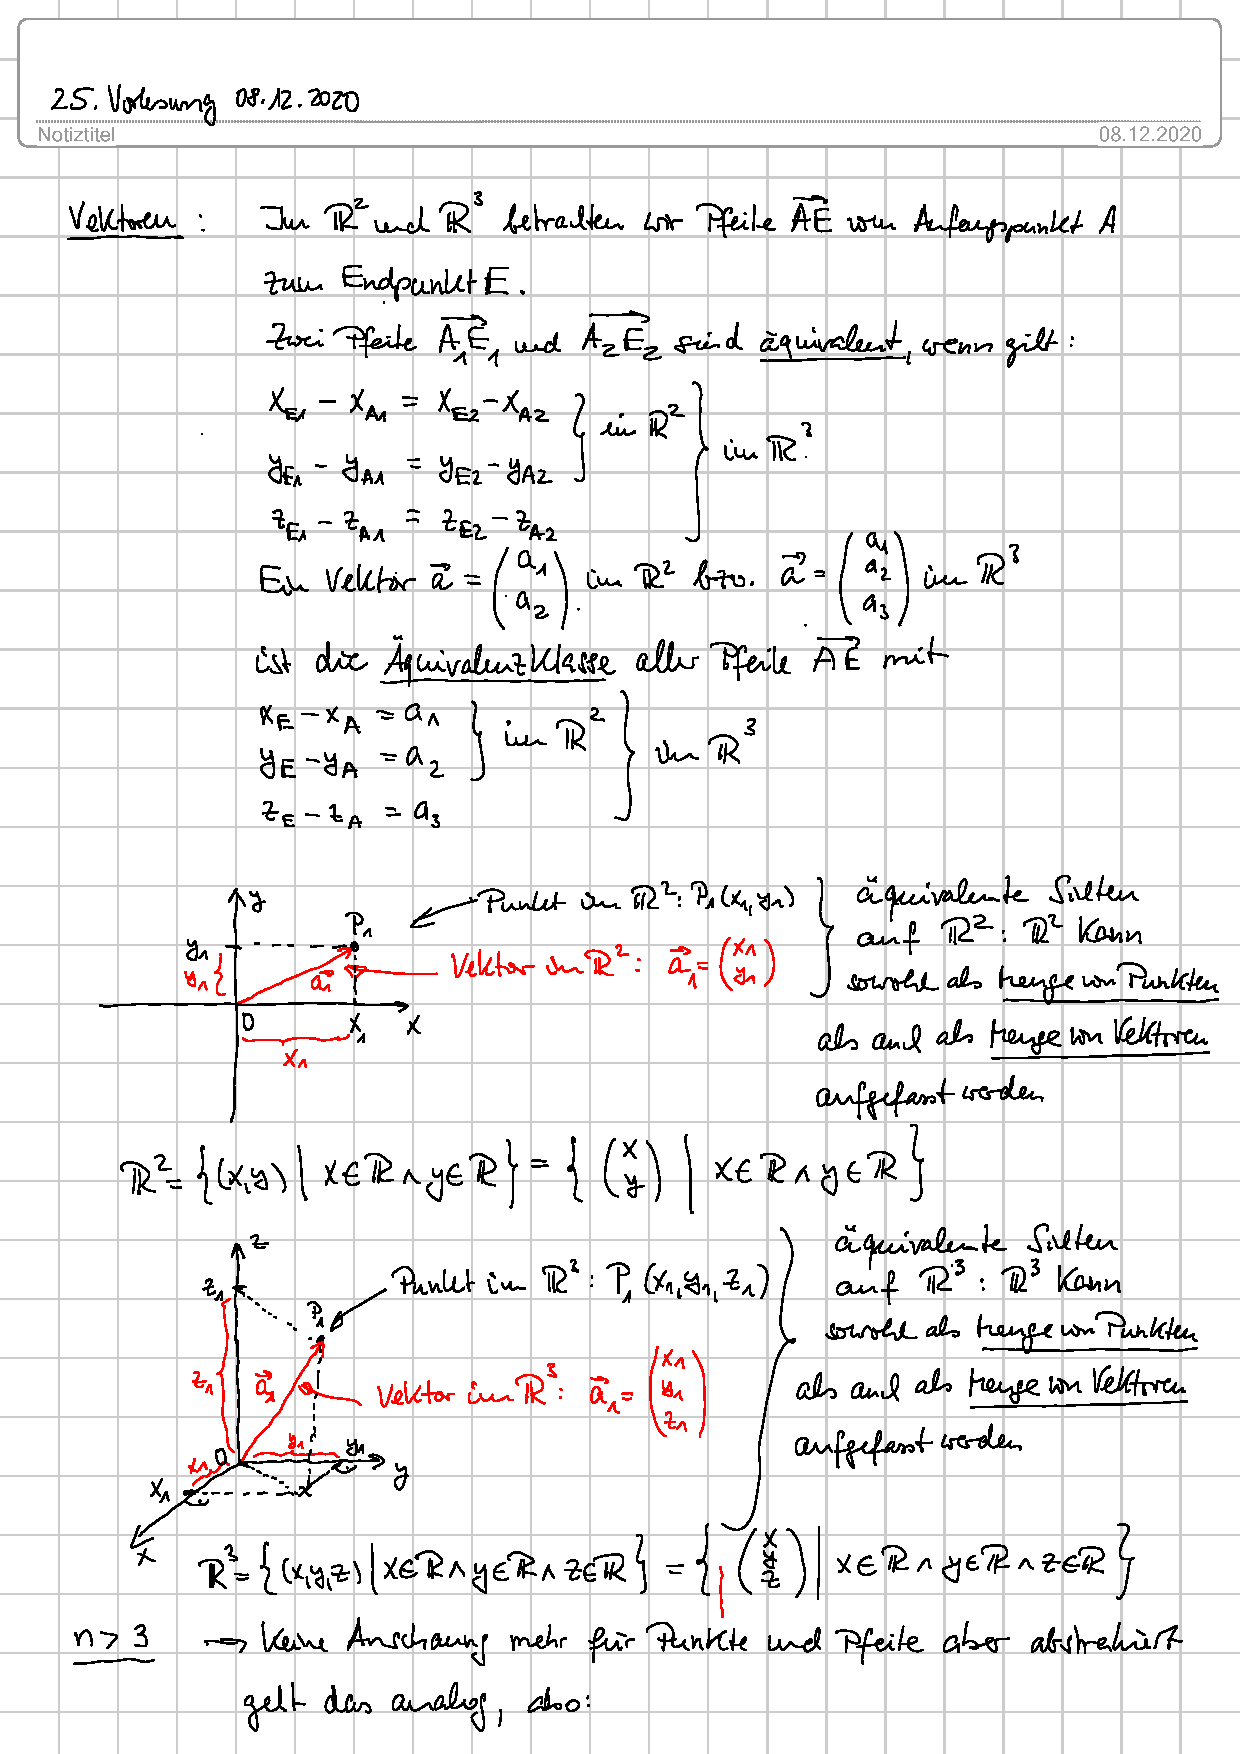
\includepdf[pages=-]{Mitschriften/25. Vorlesung 08.12.2020}

\section{Vorlesung 26 (09.12.2020)}
\subsection{Zusammenfassung: Erzeugendensystem, Basis}
\subsection{Definition: Dimension eines Vektorraums}
\subsection{Definition: Skalarprodukt, Betrag}
\subsection{Bemerkundg: Orthonormalbasis}
\subsection{Rechenregeln für Skalarprodukt und Betrag}
\subsection{Einführung: Parameterdarstellung einer Geraden}
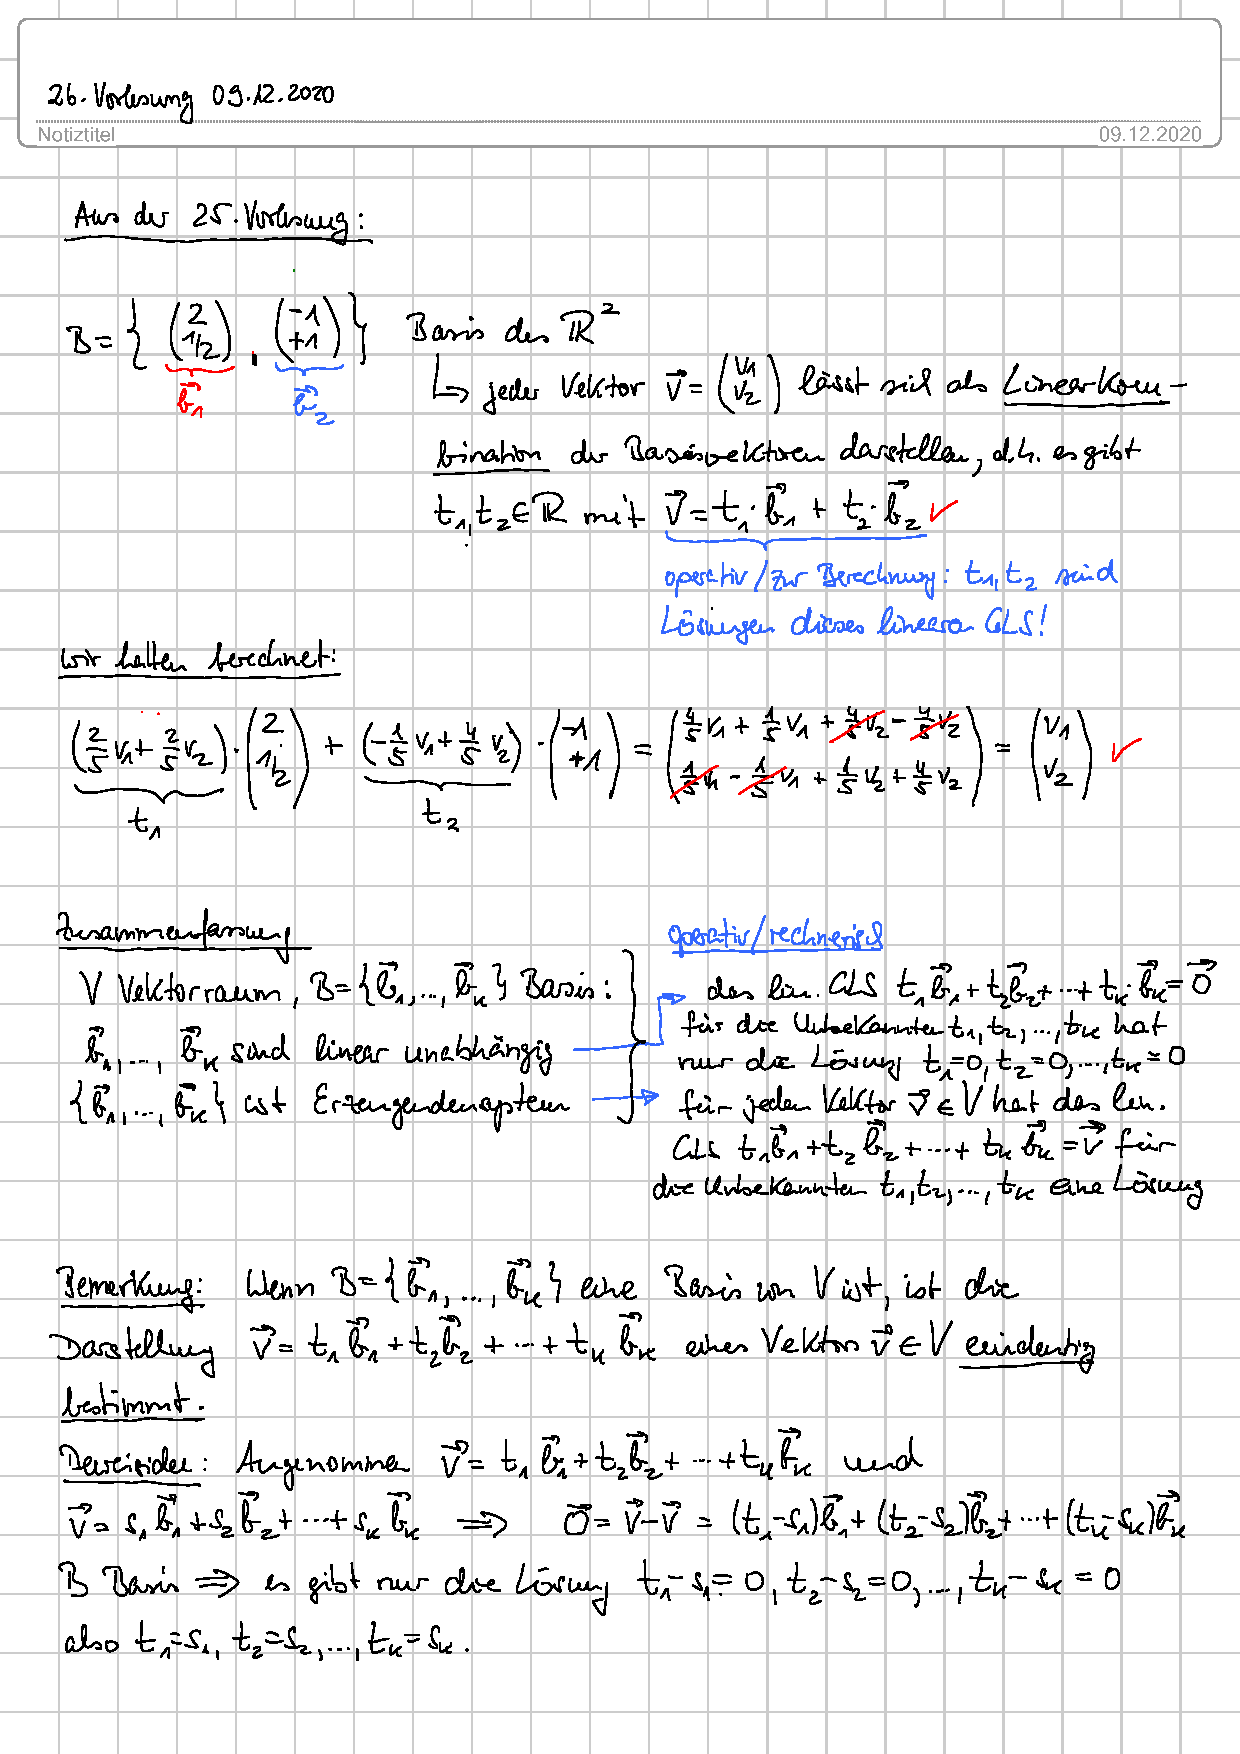
\includepdf[pages=-]{Mitschriften/26. Vorlesung 09.12.2020}

\section{Vorlesung 27 (14.12.2020)}
\subsection{Parameterdarstellung: Gerade \& Ebene}
\subsection{Orthogonalität von Vektoren/Ebenen}
\subsection{Definition: Vektorprodukt}
\subsection{Definition: Normalenvektor, Normaleneinheitsvektor}
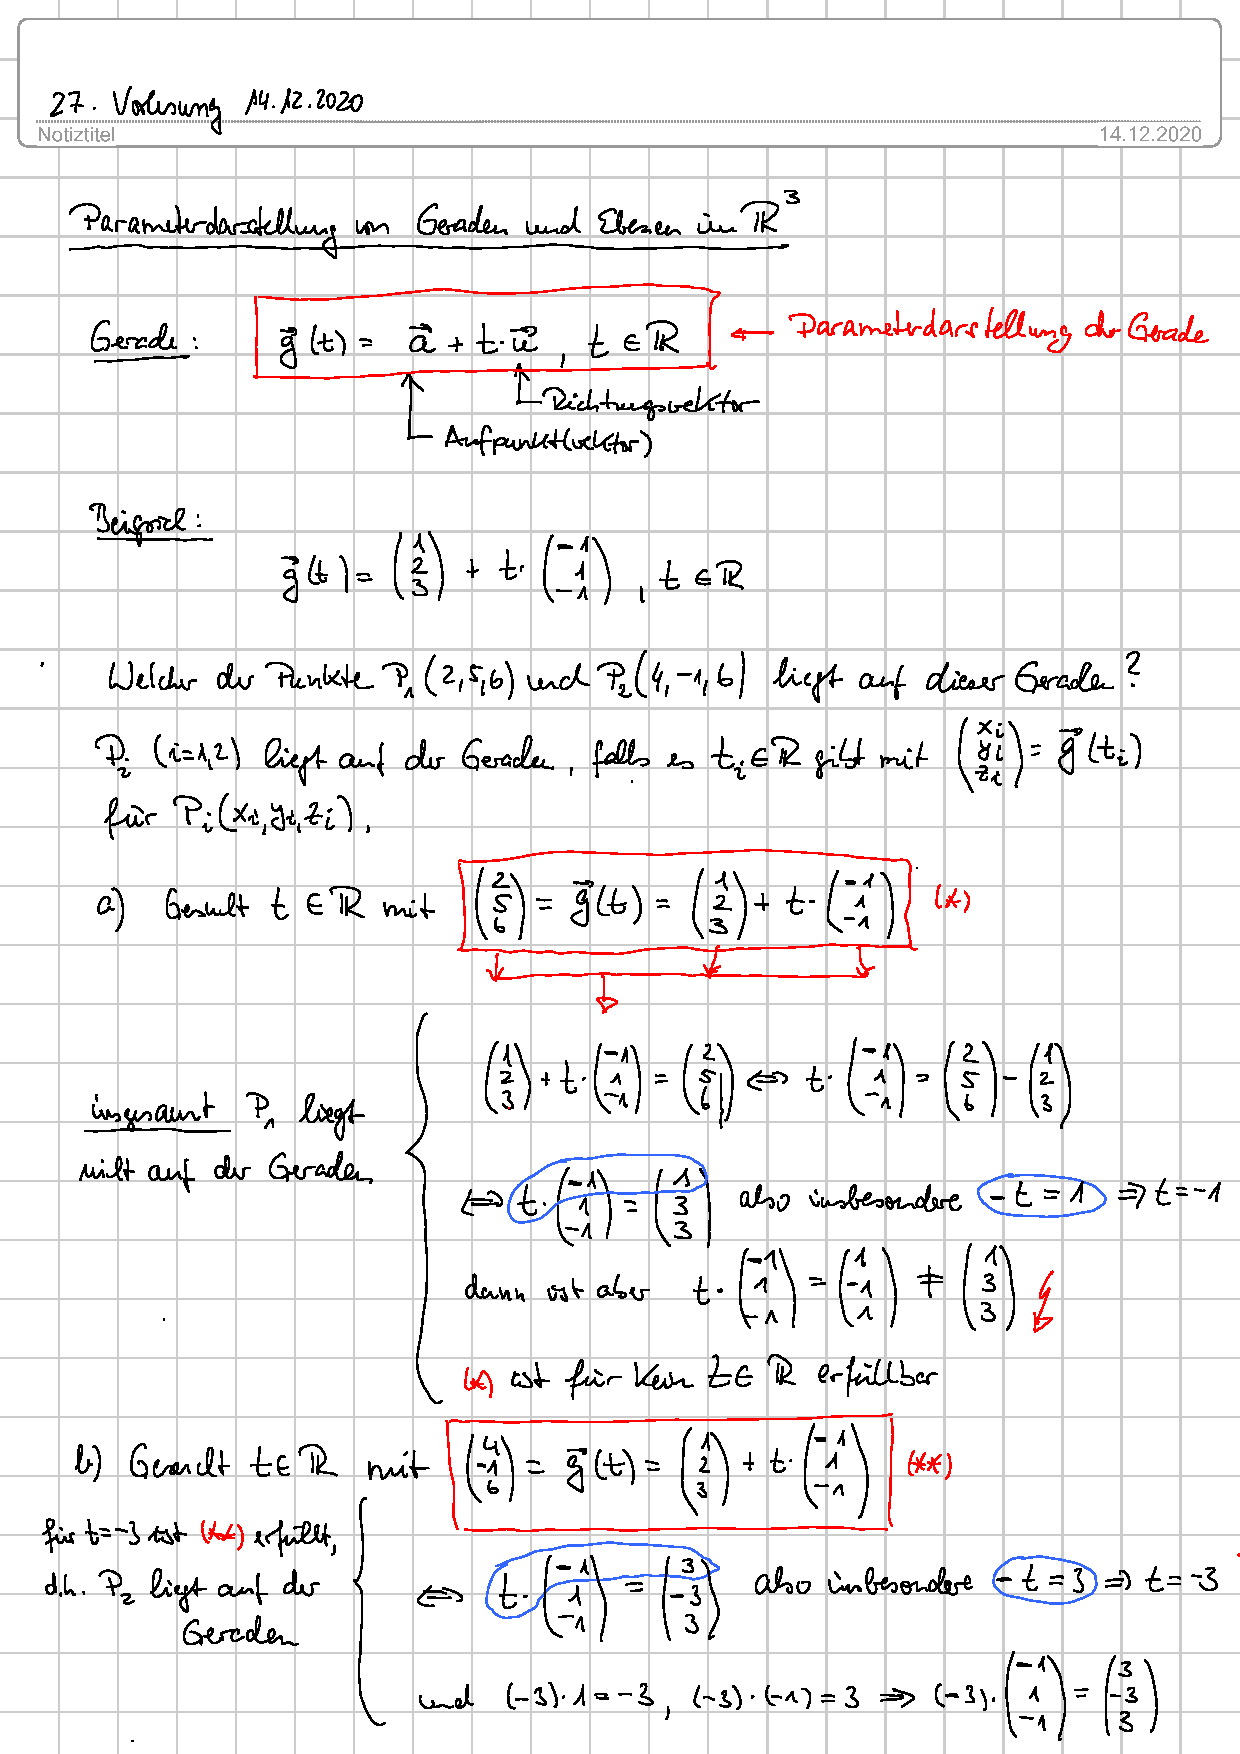
\includepdf[pages=-]{Mitschriften/27. Vorlesung 14.12.2020}

\section{Vorlesung 28 (15.12.2020)}
\subsection{Beispiele zur Parameterdarstellung von Ebenen: Punkt auf Ebene, Schnittpunkt Ebene/Gerade}
\subsection{Eigenschaften/Rechenregeln des Vektorprodukt}
\subsection{Koordinatendarstellung einer Ebene (Wandlung zu und von Parameterdarstellung)}
\subsection{Beispiel Koordinatendarstellung einer Ebene -> Schnittpunkt mit Gerade}
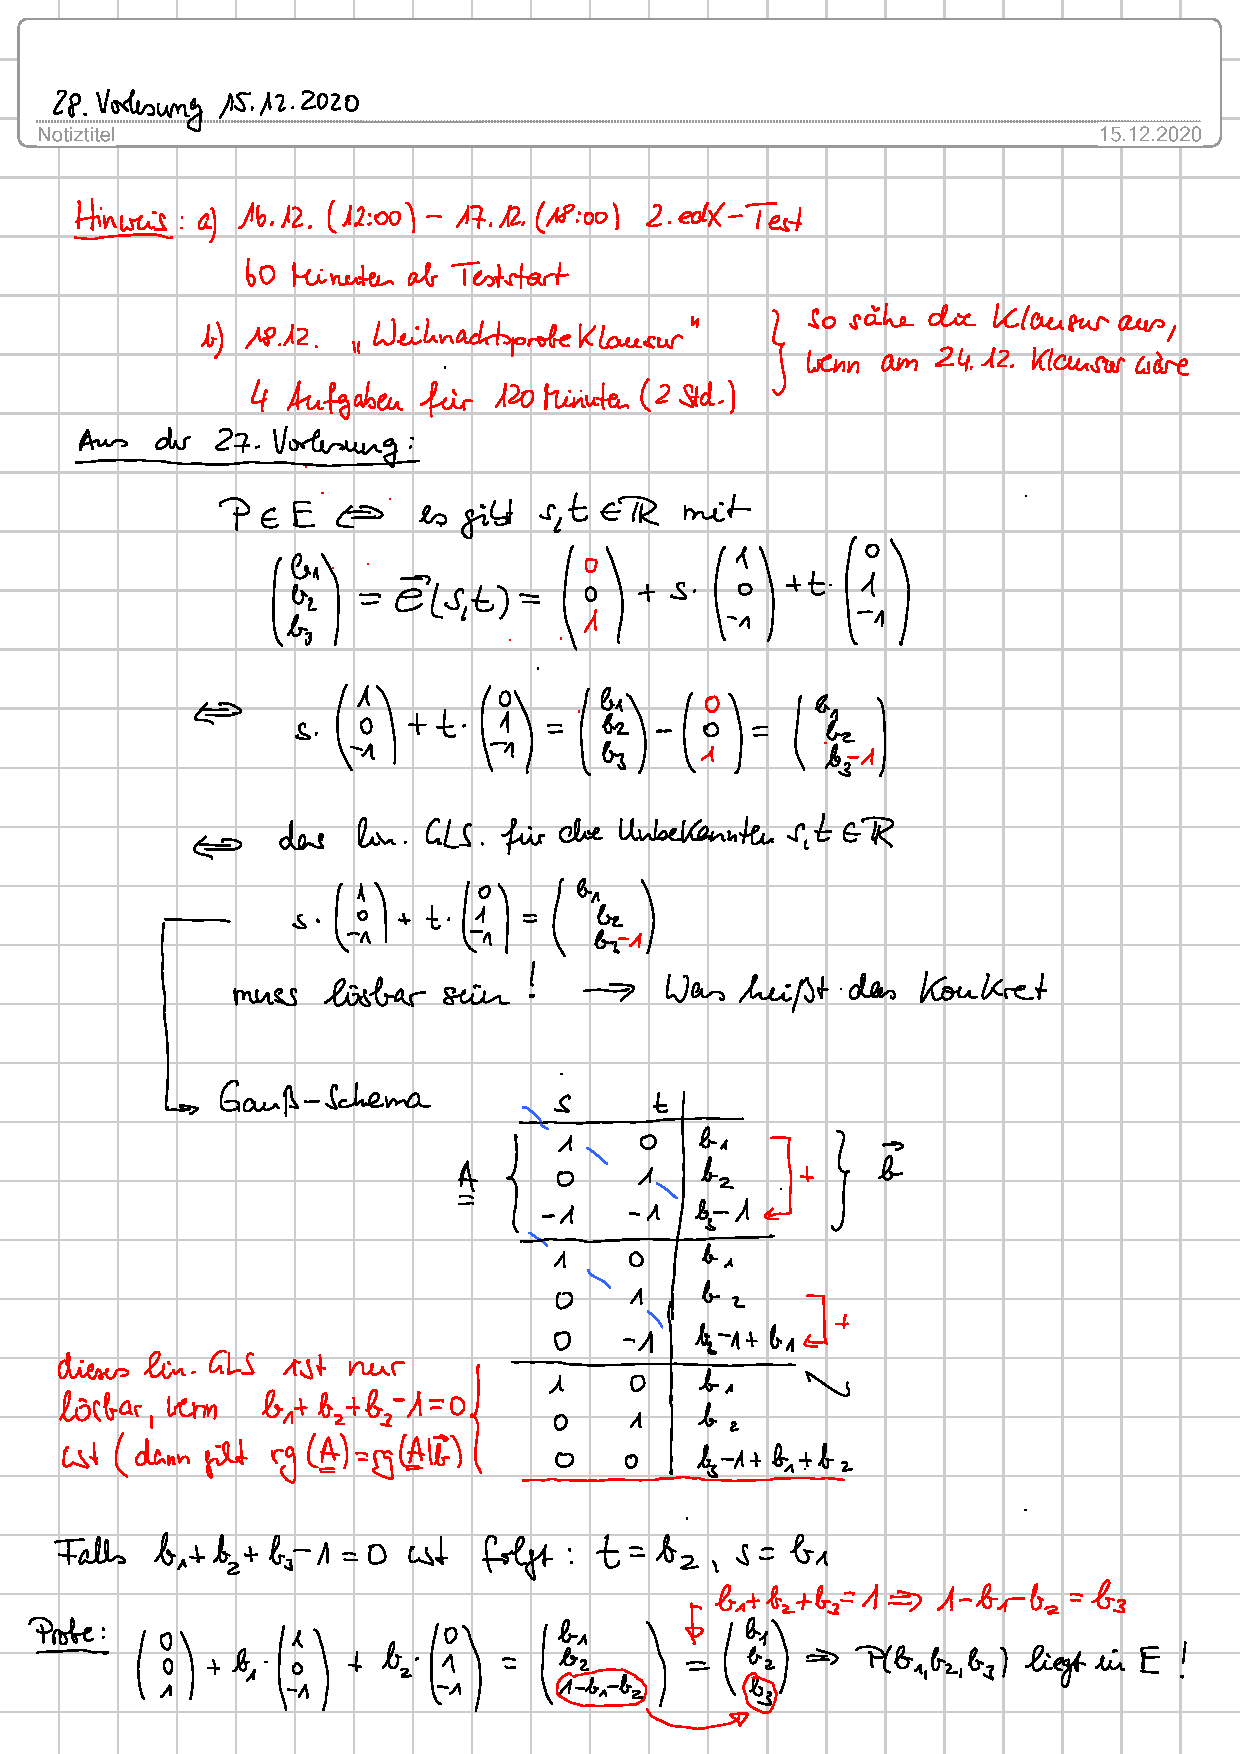
\includepdf[pages=-]{Mitschriften/28. Vorlesung 15.12.2020}

\section{Vorlesung 29 (16.12.2020)}
\subsection{Geometrie im rechtwinkligen Dreieck}
\subsection{Skalarprodukt in der Geometrie}
\subsection{Vektorprodukt in der Geometrie (Drei-Finger-Regel)}
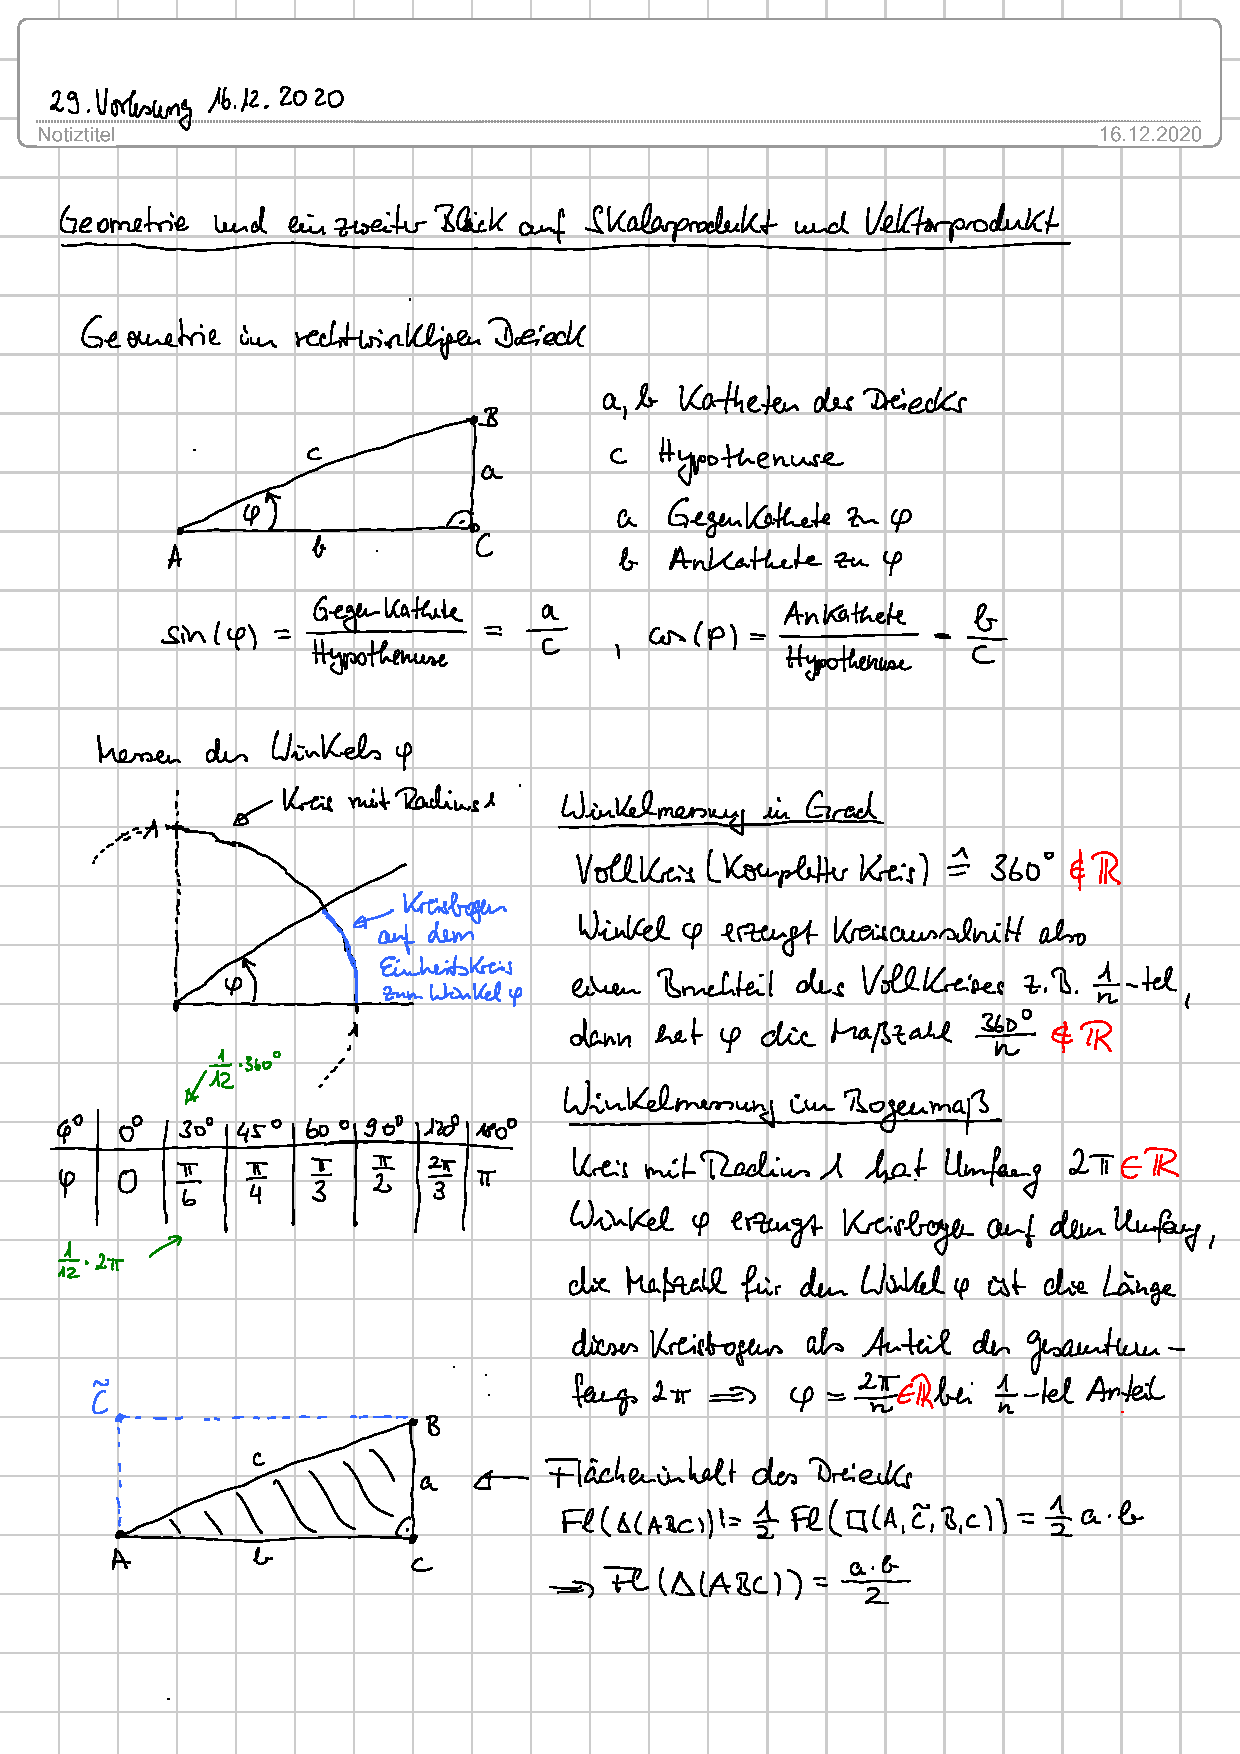
\includepdf[pages=-]{Mitschriften/29. Vorlesung 16.12.2020}

\section{Vorlesung 30 (21.12.2020)}
\subsection{Deutung von Skalarprodukt und Vektorprodukt in der Geometrie}
\subsection{Beispielaufgaben Ebenen und Geraden im Raum (Schnittgeraden, Senkrechte durch Punkt)}
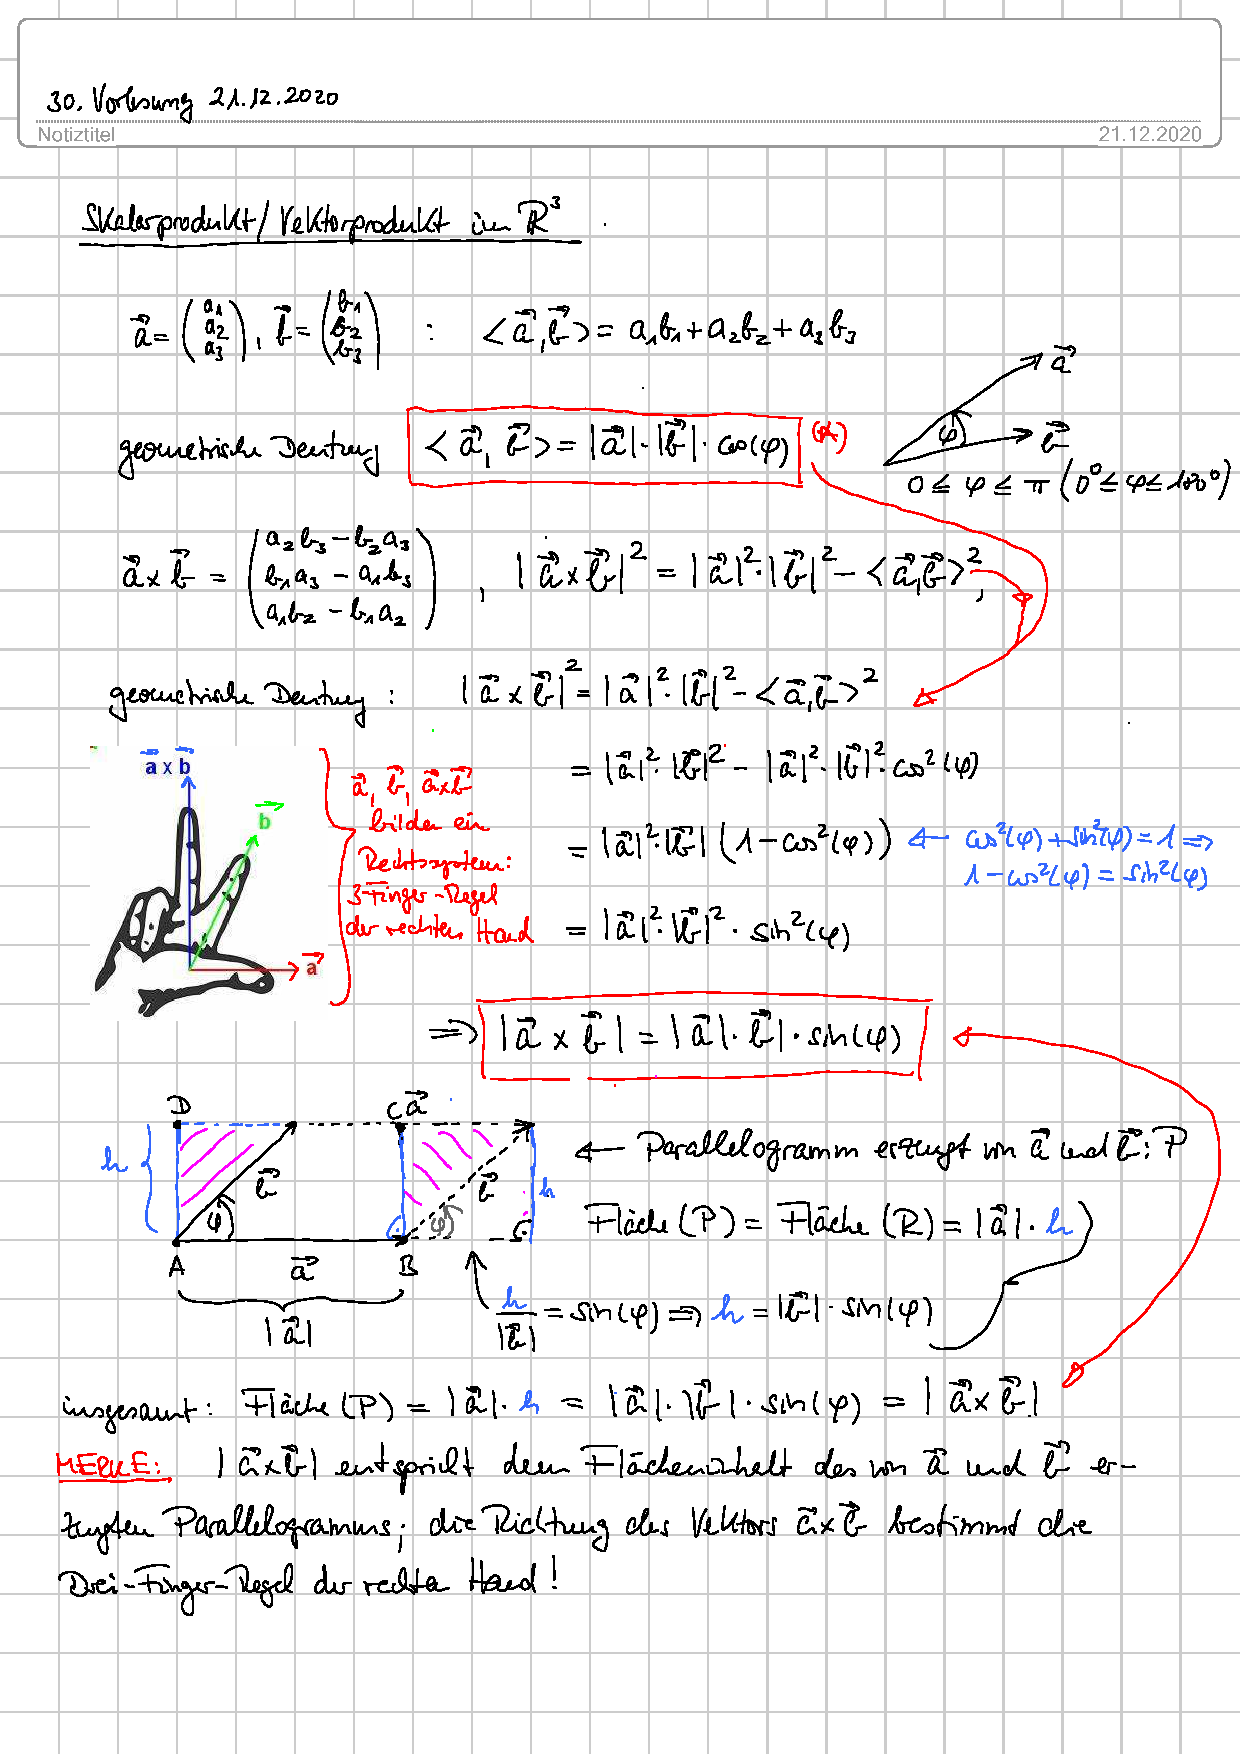
\includepdf[pages=-]{Mitschriften/30. Vorlesung 21.12.2020}

\section{Vorlesung 31 (22.12.2020)}
\subsection{Definition: Matrix}
\subsection{Rechenoperationen für Matrizen}
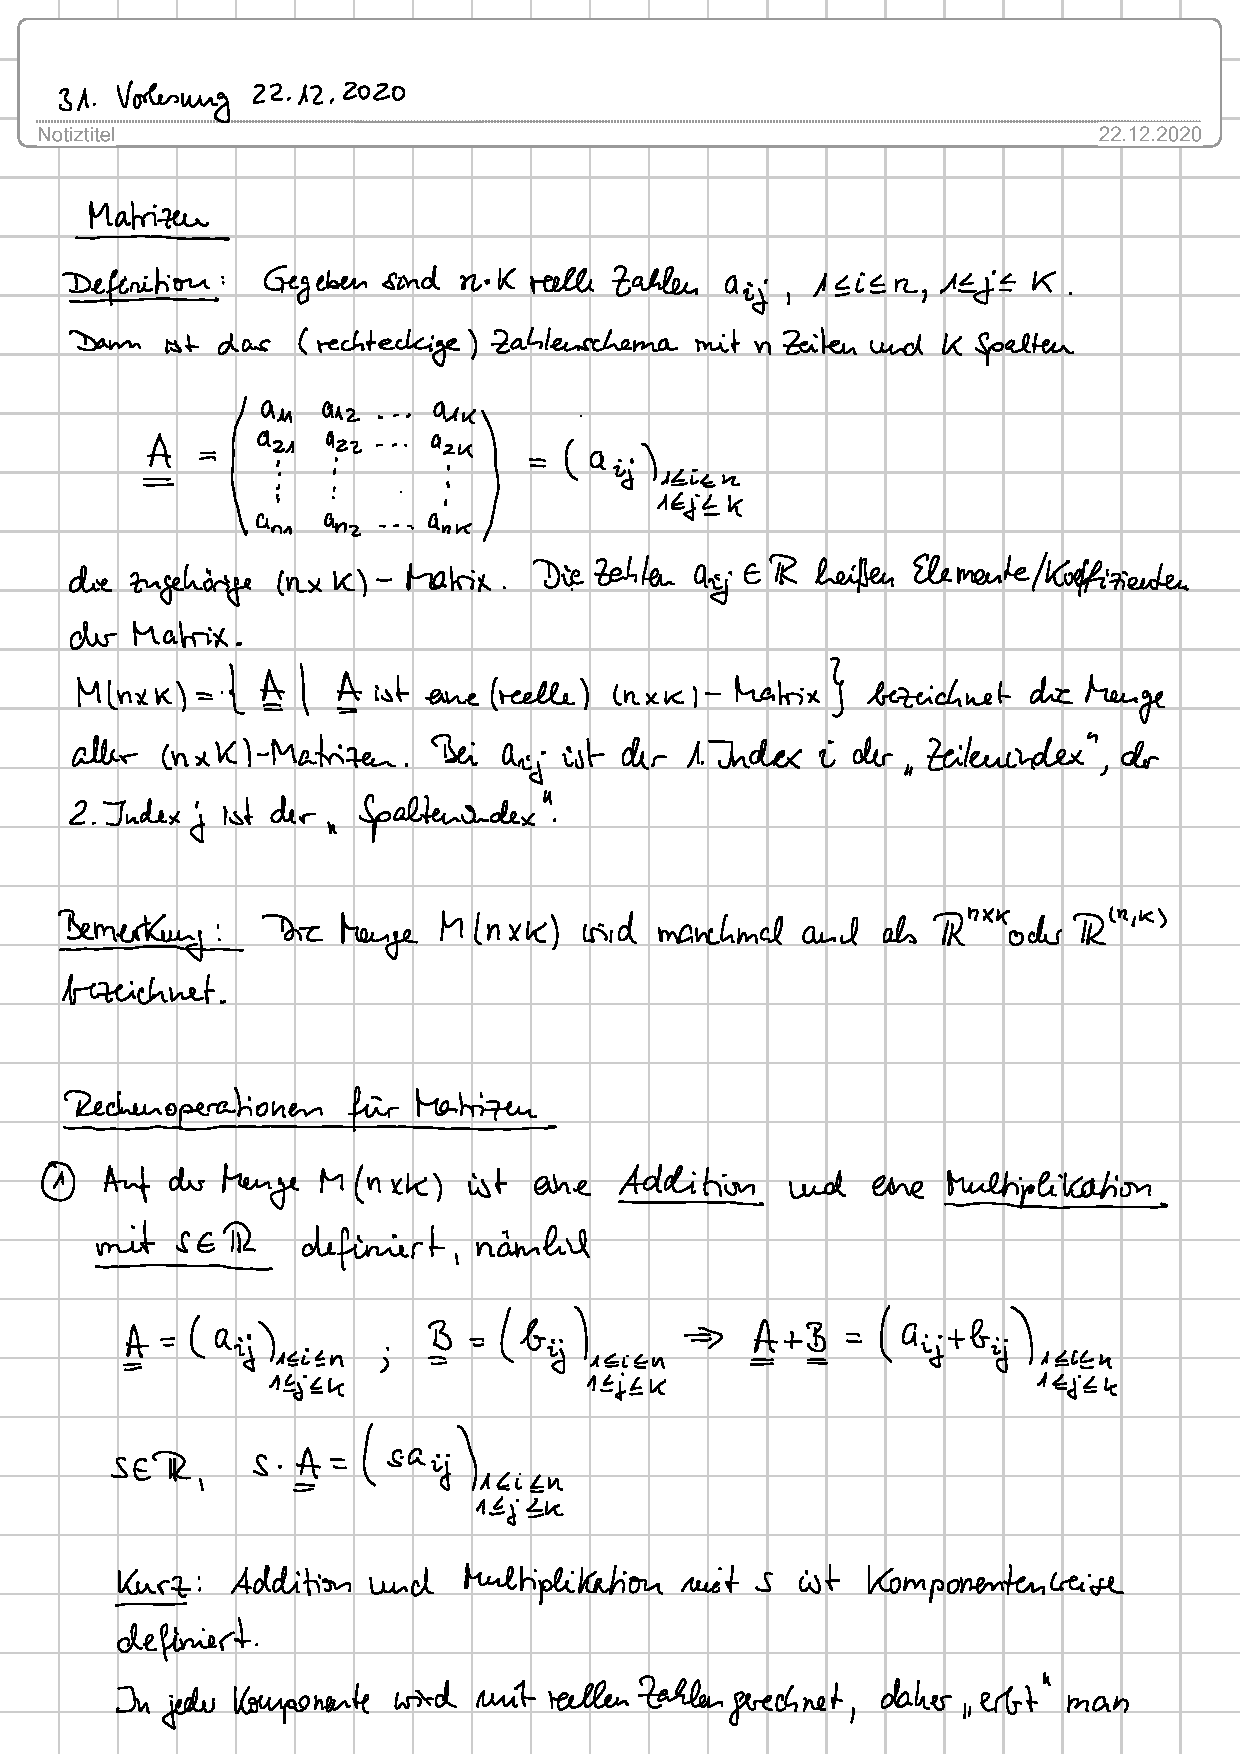
\includepdf[pages=-]{Mitschriften/31. Vorlesung 22.12.2020}

\section{Vorlesung 32 (04.01.2021)}
\subsection{Beispiele Matrixprodukt}
\subsection{Rechenregeln für Matrixprodukt}
\subsection{transponierte Matrix}
\subsection{quadratische Matrix, Nullmatrix, Einheitsmatrix}
\subsection{Definition: Determinante einer Matrix (2x2-Matrix)}
\subsection{Definition: invertierbare/inverse Matrix}
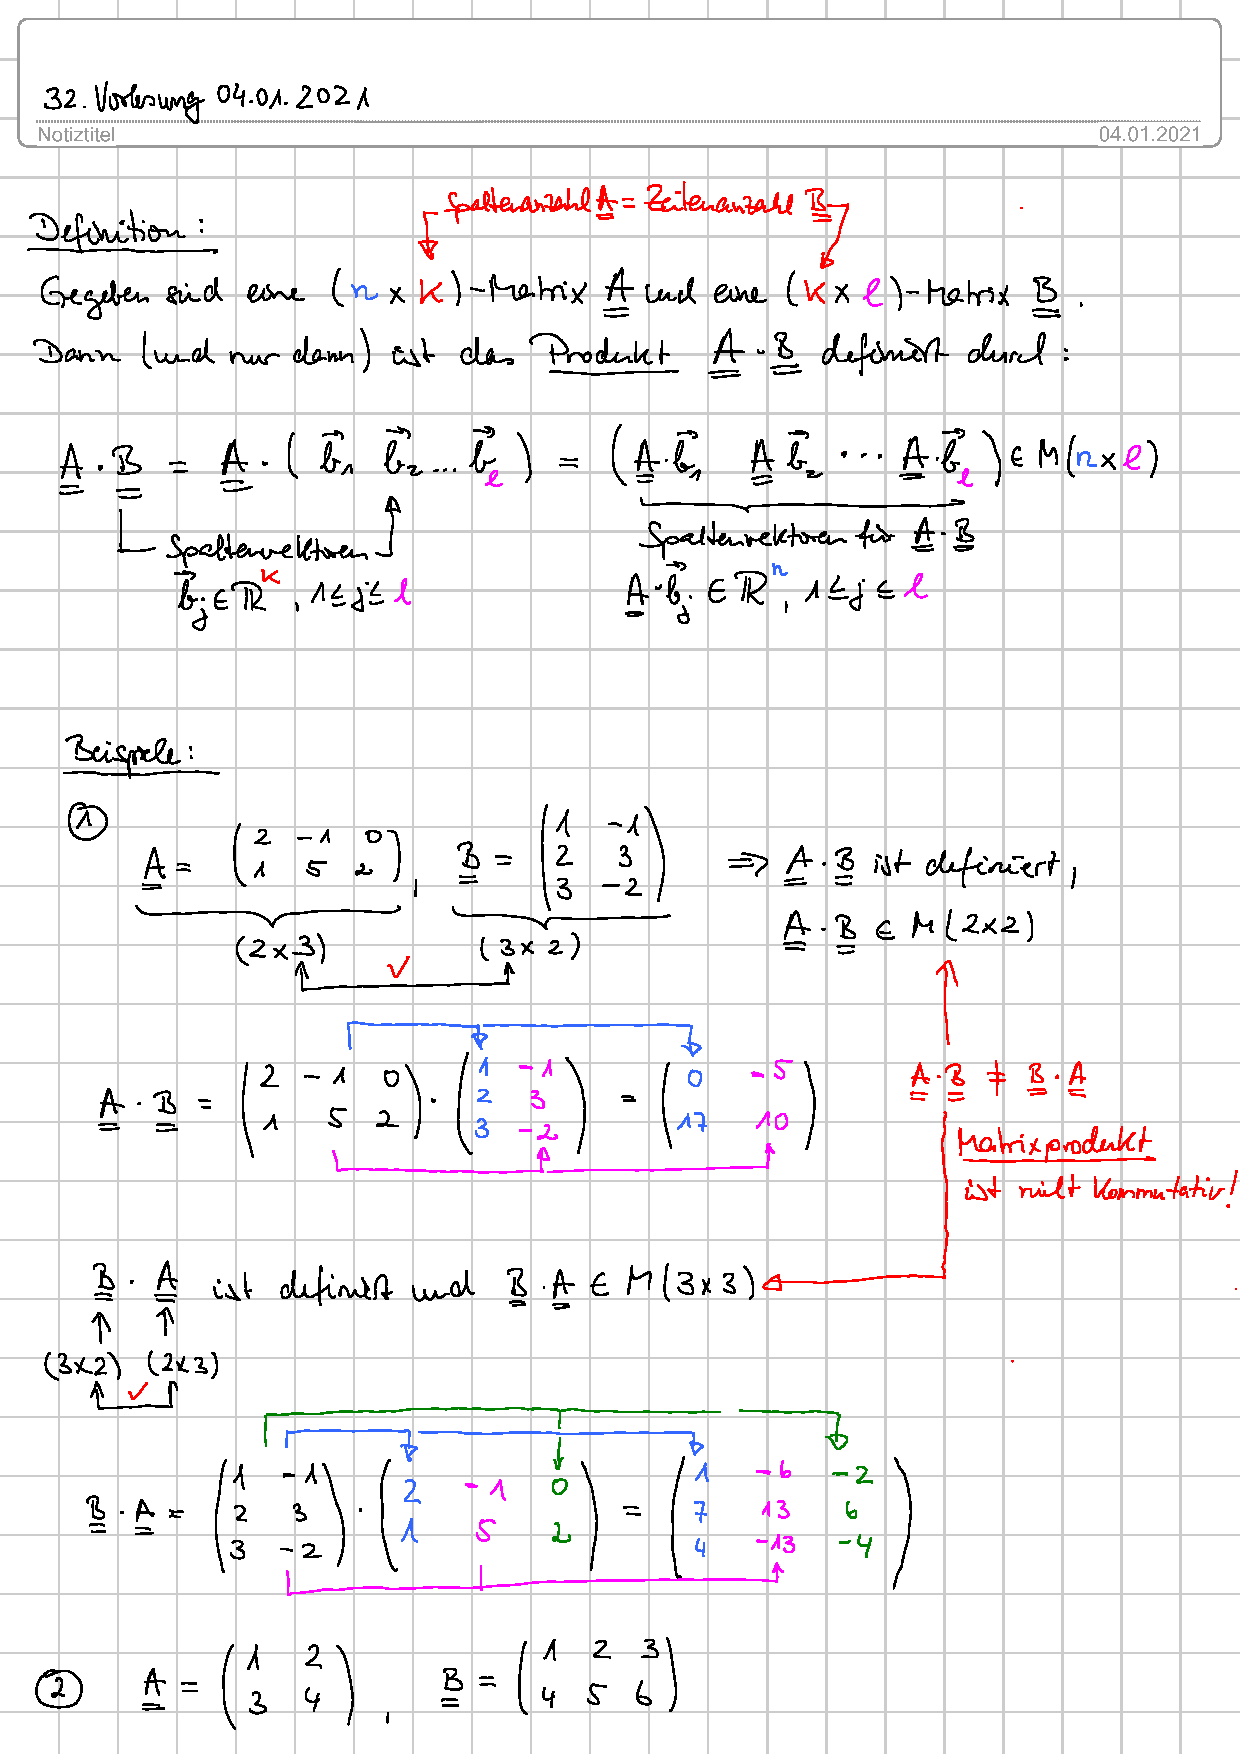
\includepdf[pages=-]{Mitschriften/32. Vorlesung 04.01.2021}

\section{Vorlesung 33 (05.01.2021)}
\subsection{Bestimmen der Inversen Matrix (im Allgemeinen und 2x2-Matrizen)}
\subsection{Eigenschaften/Rechenregeln der Determinante (2x2)}
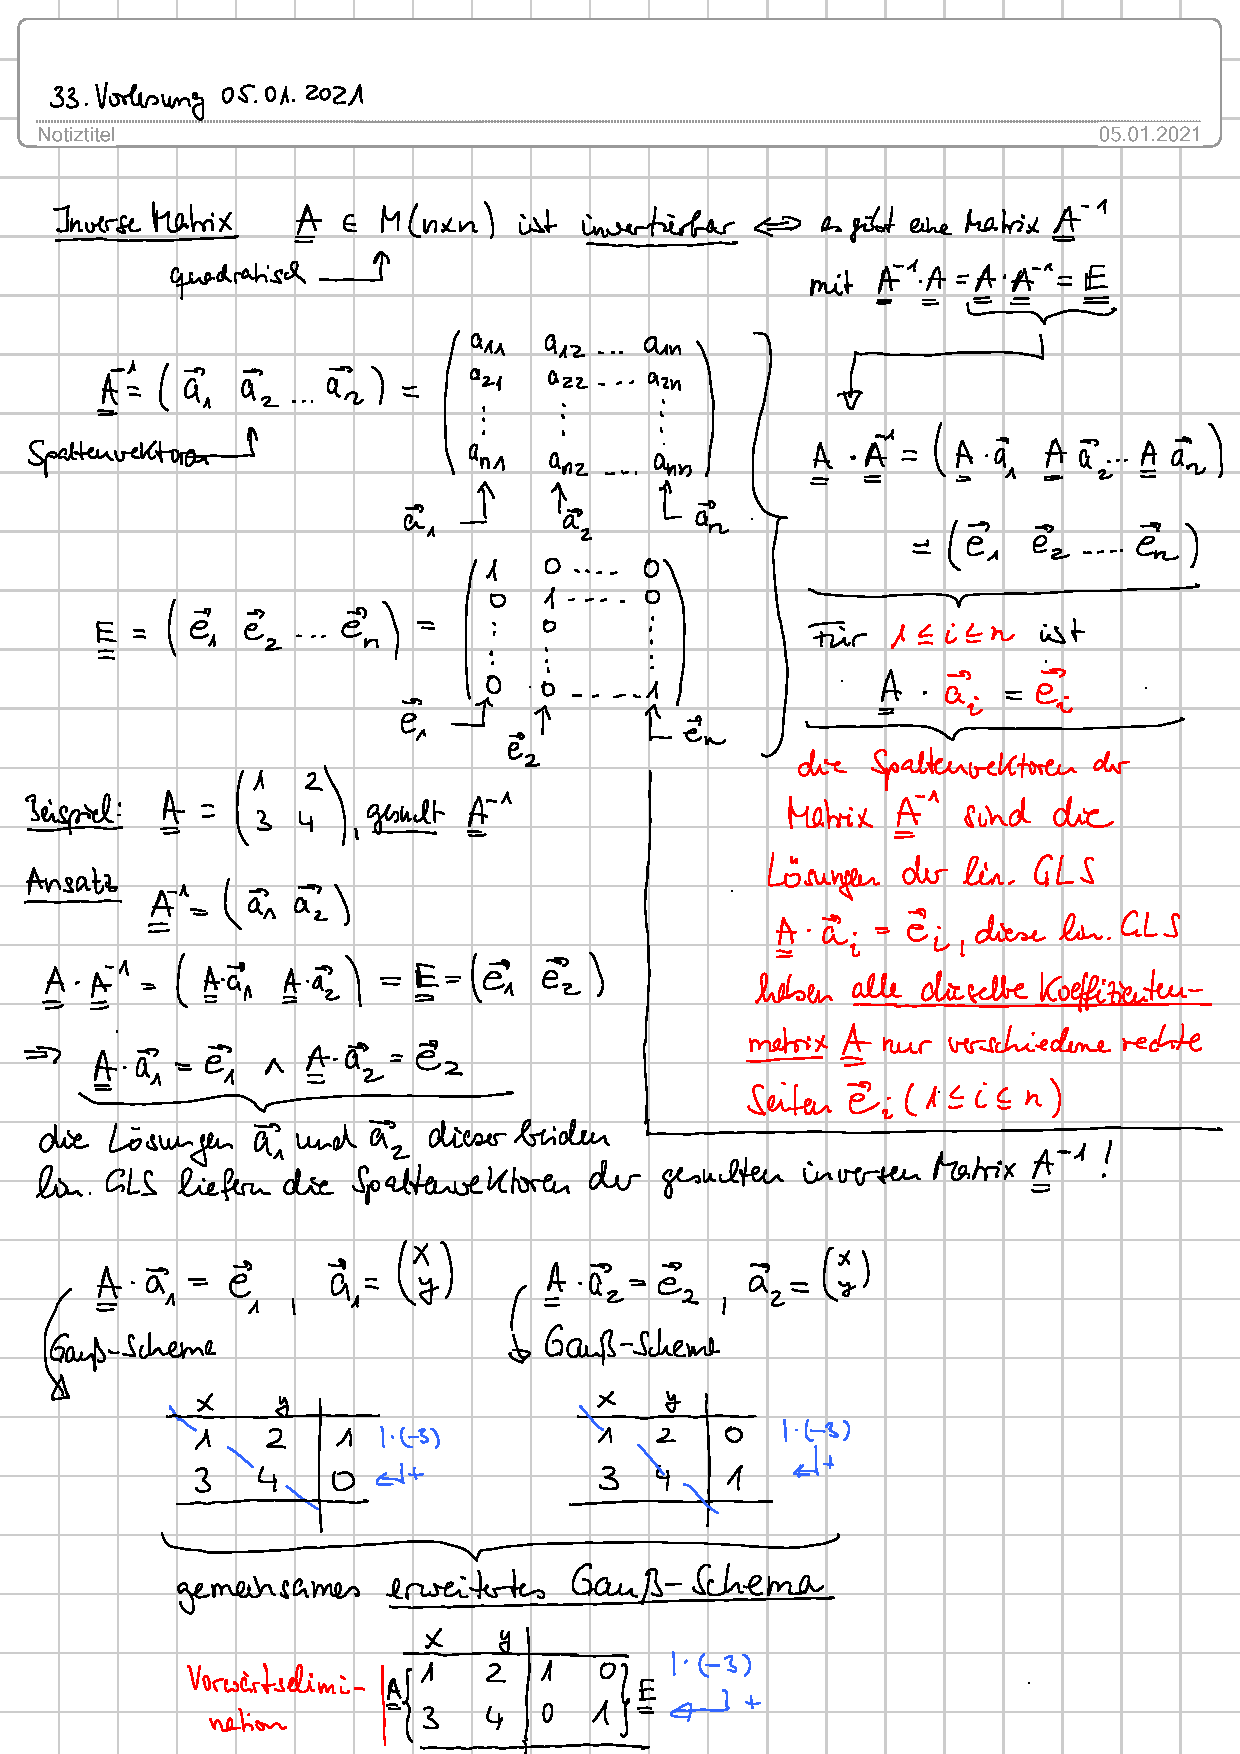
\includepdf[pages=-]{Mitschriften/33. Vorlesung 05.01.2021}

\section{Vorlesung 34 (06.01.2021)}
\subsection{(forts.) Eigenschaften/Rechenregeln der Determinante (2x2)}
\subsection{Definition: Determinante einer Matrix (nxn-Matrix)}
\subsection{Eigenschaften/Rechenregeln der Determinante (nxn)}
\subsection{Beispiele für Determinanten}
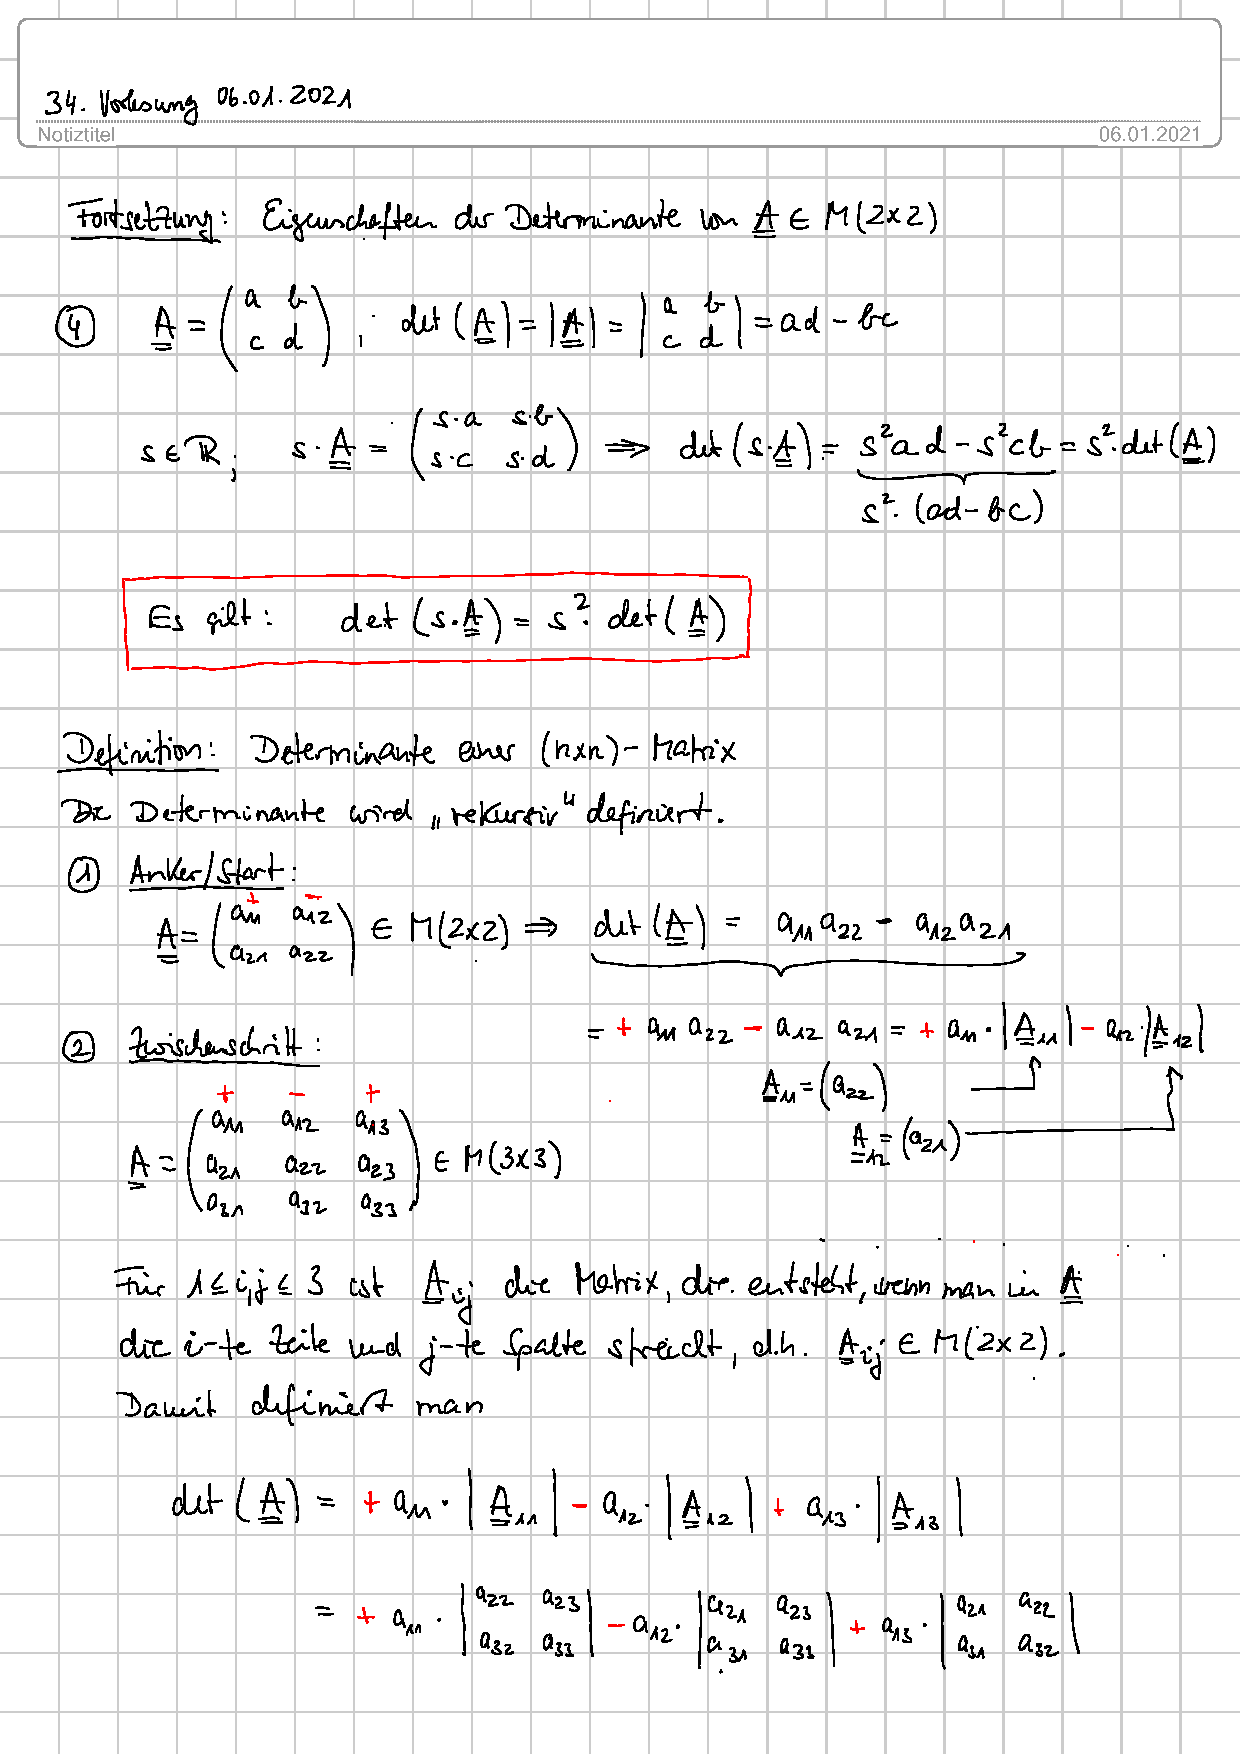
\includepdf[pages=-]{Mitschriften/34. Vorlesung 06.01.2021}



\end{document}